\documentclass{book}
\usepackage[a4paper,top=2.5cm,bottom=2.5cm,left=2.5cm,right=2.5cm]{geometry}
\usepackage{makeidx}
\usepackage{natbib}
\usepackage{graphicx}
\usepackage{multicol}
\usepackage{float}
\usepackage{listings}
\usepackage{color}
\usepackage{ifthen}
\usepackage[table]{xcolor}
\usepackage{textcomp}
\usepackage{alltt}
\usepackage{ifpdf}
\ifpdf
\usepackage[pdftex,
            pagebackref=true,
            colorlinks=true,
            linkcolor=blue,
            unicode
           ]{hyperref}
\else
\usepackage[ps2pdf,
            pagebackref=true,
            colorlinks=true,
            linkcolor=blue,
            unicode
           ]{hyperref}
\usepackage{pspicture}
\fi
\usepackage[utf8]{inputenc}
\usepackage[french]{babel}

\usepackage{mathptmx}
\usepackage[scaled=.90]{helvet}
\usepackage{courier}
\usepackage{sectsty}
\usepackage{amssymb}
\usepackage[titles]{tocloft}
\usepackage{doxygen}
\lstset{language=C++,inputencoding=utf8,basicstyle=\footnotesize,breaklines=true,breakatwhitespace=true,tabsize=8,numbers=left }
\makeindex
\setcounter{tocdepth}{3}
\renewcommand{\footrulewidth}{0.4pt}
\renewcommand{\familydefault}{\sfdefault}
\hfuzz=15pt
\setlength{\emergencystretch}{15pt}
\hbadness=750
\tolerance=750
\begin{document}
\hypersetup{pageanchor=false,citecolor=blue}
\begin{titlepage}
\vspace*{7cm}
\begin{center}
{\Large Java }\\
\vspace*{1cm}
{\large Généré par Doxygen 1.8.1.2}\\
\vspace*{0.5cm}
{\small Mercredi Janvier 8 2014 09:35:56}\\
\end{center}
\end{titlepage}
\clearemptydoublepage
\pagenumbering{roman}
\tableofcontents
\clearemptydoublepage
\pagenumbering{arabic}
\hypersetup{pageanchor=true,citecolor=blue}
\chapter{Index des classes}
\section{Hiérarchie des classes}
Cette liste d'héritage est classée approximativement par ordre alphabétique \-:\begin{DoxyCompactList}
\item \contentsline{section}{serveur.\-I\-Arene}{\pageref{interfaceserveur_1_1_i_arene}}{}
\begin{DoxyCompactList}
\item \contentsline{section}{serveur.\-Arene}{\pageref{classserveur_1_1_arene}}{}
\end{DoxyCompactList}
\item \contentsline{section}{individu.\-combattant.\-I\-Combattant}{\pageref{interfaceindividu_1_1combattant_1_1_i_combattant}}{}
\begin{DoxyCompactList}
\item \contentsline{section}{individu.\-combattant.\-Combattant}{\pageref{classindividu_1_1combattant_1_1_combattant}}{}
\begin{DoxyCompactList}
\item \contentsline{section}{individu.\-combattant.\-Barde}{\pageref{classindividu_1_1combattant_1_1_barde}}{}
\item \contentsline{section}{individu.\-combattant.\-Capitaine}{\pageref{classindividu_1_1combattant_1_1_capitaine}}{}
\item \contentsline{section}{individu.\-combattant.\-Cyborg}{\pageref{classindividu_1_1combattant_1_1_cyborg}}{}
\item \contentsline{section}{individu.\-combattant.\-Mascotte}{\pageref{classindividu_1_1combattant_1_1_mascotte}}{}
\item \contentsline{section}{individu.\-combattant.\-Spadassin}{\pageref{classindividu_1_1combattant_1_1_spadassin}}{}
\end{DoxyCompactList}
\end{DoxyCompactList}
\item \contentsline{section}{controle.\-I\-Console}{\pageref{interfacecontrole_1_1_i_console}}{}
\begin{DoxyCompactList}
\item \contentsline{section}{controle.\-Console}{\pageref{classcontrole_1_1_console}}{}
\end{DoxyCompactList}
\item \contentsline{section}{interaction.\-I\-Duel}{\pageref{interfaceinteraction_1_1_i_duel}}{}
\begin{DoxyCompactList}
\item \contentsline{section}{interaction.\-Duel\-Basic}{\pageref{classinteraction_1_1_duel_basic}}{}
\end{DoxyCompactList}
\item \contentsline{section}{individu.\-I\-Element}{\pageref{interfaceindividu_1_1_i_element}}{}
\begin{DoxyCompactList}
\item \contentsline{section}{individu.\-Element}{\pageref{classindividu_1_1_element}}{}
\begin{DoxyCompactList}
\item \contentsline{section}{individu.\-combattant.\-Combattant}{\pageref{classindividu_1_1combattant_1_1_combattant}}{}
\item \contentsline{section}{individu.\-equipement.\-Equipement}{\pageref{classindividu_1_1equipement_1_1_equipement}}{}
\begin{DoxyCompactList}
\item \contentsline{section}{individu.\-equipement.\-Bottes}{\pageref{classindividu_1_1equipement_1_1_bottes}}{}
\item \contentsline{section}{individu.\-equipement.\-Canne}{\pageref{classindividu_1_1equipement_1_1_canne}}{}
\item \contentsline{section}{individu.\-equipement.\-Chapeau\-De\-Paille}{\pageref{classindividu_1_1equipement_1_1_chapeau_de_paille}}{}
\item \contentsline{section}{individu.\-equipement.\-Plastron}{\pageref{classindividu_1_1equipement_1_1_plastron}}{}
\item \contentsline{section}{individu.\-equipement.\-Sabre}{\pageref{classindividu_1_1equipement_1_1_sabre}}{}
\end{DoxyCompactList}
\end{DoxyCompactList}
\end{DoxyCompactList}
\item \contentsline{section}{interface\-Graphique.\-I\-H\-M}{\pageref{classinterface_graphique_1_1_i_h_m}}{}
\item \contentsline{section}{individu.\-combattant.\-Liste\-Equipements}{\pageref{classindividu_1_1combattant_1_1_liste_equipements}}{}
\item \contentsline{section}{interface\-Graphique.\-Point\-Comp}{\pageref{classinterface_graphique_1_1_point_comp}}{}
\item \contentsline{section}{controle.\-Strategie}{\pageref{classcontrole_1_1_strategie}}{}
\item \contentsline{section}{Test\-Console}{\pageref{class_test_console}}{}
\item \contentsline{section}{Test\-Console\-Barde}{\pageref{class_test_console_barde}}{}
\item \contentsline{section}{Test\-Console\-Bottes}{\pageref{class_test_console_bottes}}{}
\item \contentsline{section}{Test\-Console\-Canne}{\pageref{class_test_console_canne}}{}
\item \contentsline{section}{Test\-Console\-Capitaine}{\pageref{class_test_console_capitaine}}{}
\item \contentsline{section}{Test\-Console\-Chap\-De\-Paille}{\pageref{class_test_console_chap_de_paille}}{}
\item \contentsline{section}{Test\-Console\-Cyborg}{\pageref{class_test_console_cyborg}}{}
\item \contentsline{section}{Test\-Console\-Mascotte}{\pageref{class_test_console_mascotte}}{}
\item \contentsline{section}{Test\-Console\-Plastron}{\pageref{class_test_console_plastron}}{}
\item \contentsline{section}{Test\-Console\-Sabre}{\pageref{class_test_console_sabre}}{}
\item \contentsline{section}{Test\-Console\-Spadassin}{\pageref{class_test_console_spadassin}}{}
\item \contentsline{section}{Test\-I\-H\-M}{\pageref{class_test_i_h_m}}{}
\item \contentsline{section}{Test\-Serveur}{\pageref{class_test_serveur}}{}
\item \contentsline{section}{serveur.\-Arene.\-Timeout\-Op}{\pageref{classserveur_1_1_arene_1_1_timeout_op}}{}
\item \contentsline{section}{utilitaires.\-Utilitaire\-Console}{\pageref{classutilitaires_1_1_utilitaire_console}}{}
\item \contentsline{section}{interface\-Graphique.\-Vue\-Element}{\pageref{classinterface_graphique_1_1_vue_element}}{}
\end{DoxyCompactList}

\chapter{Index des classes}
\section{Liste des classes}
Liste des classes, structures, unions et interfaces avec une brève description \-:\begin{DoxyCompactList}
\item\contentsline{section}{\hyperlink{classserveur_1_1_arene}{serveur.\-Arene} }{\pageref{classserveur_1_1_arene}}{}
\item\contentsline{section}{\hyperlink{classindividu_1_1combattant_1_1_barde}{individu.\-combattant.\-Barde} }{\pageref{classindividu_1_1combattant_1_1_barde}}{}
\item\contentsline{section}{\hyperlink{classindividu_1_1equipement_1_1_bottes}{individu.\-equipement.\-Bottes} }{\pageref{classindividu_1_1equipement_1_1_bottes}}{}
\item\contentsline{section}{\hyperlink{classindividu_1_1equipement_1_1_canne}{individu.\-equipement.\-Canne} }{\pageref{classindividu_1_1equipement_1_1_canne}}{}
\item\contentsline{section}{\hyperlink{classindividu_1_1combattant_1_1_capitaine}{individu.\-combattant.\-Capitaine} }{\pageref{classindividu_1_1combattant_1_1_capitaine}}{}
\item\contentsline{section}{\hyperlink{classindividu_1_1equipement_1_1_chapeau_de_paille}{individu.\-equipement.\-Chapeau\-De\-Paille} }{\pageref{classindividu_1_1equipement_1_1_chapeau_de_paille}}{}
\item\contentsline{section}{\hyperlink{classindividu_1_1combattant_1_1_combattant}{individu.\-combattant.\-Combattant} }{\pageref{classindividu_1_1combattant_1_1_combattant}}{}
\item\contentsline{section}{\hyperlink{classcontrole_1_1_console}{controle.\-Console} }{\pageref{classcontrole_1_1_console}}{}
\item\contentsline{section}{\hyperlink{classindividu_1_1combattant_1_1_cyborg}{individu.\-combattant.\-Cyborg} }{\pageref{classindividu_1_1combattant_1_1_cyborg}}{}
\item\contentsline{section}{\hyperlink{classinteraction_1_1_duel_basic}{interaction.\-Duel\-Basic} }{\pageref{classinteraction_1_1_duel_basic}}{}
\item\contentsline{section}{\hyperlink{classindividu_1_1_element}{individu.\-Element} }{\pageref{classindividu_1_1_element}}{}
\item\contentsline{section}{\hyperlink{classindividu_1_1equipement_1_1_equipement}{individu.\-equipement.\-Equipement} }{\pageref{classindividu_1_1equipement_1_1_equipement}}{}
\item\contentsline{section}{\hyperlink{interfaceserveur_1_1_i_arene}{serveur.\-I\-Arene} }{\pageref{interfaceserveur_1_1_i_arene}}{}
\item\contentsline{section}{\hyperlink{interfaceindividu_1_1combattant_1_1_i_combattant}{individu.\-combattant.\-I\-Combattant} }{\pageref{interfaceindividu_1_1combattant_1_1_i_combattant}}{}
\item\contentsline{section}{\hyperlink{interfacecontrole_1_1_i_console}{controle.\-I\-Console} }{\pageref{interfacecontrole_1_1_i_console}}{}
\item\contentsline{section}{\hyperlink{interfaceinteraction_1_1_i_duel}{interaction.\-I\-Duel} }{\pageref{interfaceinteraction_1_1_i_duel}}{}
\item\contentsline{section}{\hyperlink{interfaceindividu_1_1_i_element}{individu.\-I\-Element} }{\pageref{interfaceindividu_1_1_i_element}}{}
\item\contentsline{section}{\hyperlink{classinterface_graphique_1_1_i_h_m}{interface\-Graphique.\-I\-H\-M} }{\pageref{classinterface_graphique_1_1_i_h_m}}{}
\item\contentsline{section}{\hyperlink{classindividu_1_1combattant_1_1_liste_equipements}{individu.\-combattant.\-Liste\-Equipements} }{\pageref{classindividu_1_1combattant_1_1_liste_equipements}}{}
\item\contentsline{section}{\hyperlink{classindividu_1_1combattant_1_1_mascotte}{individu.\-combattant.\-Mascotte} }{\pageref{classindividu_1_1combattant_1_1_mascotte}}{}
\item\contentsline{section}{\hyperlink{classindividu_1_1equipement_1_1_plastron}{individu.\-equipement.\-Plastron} }{\pageref{classindividu_1_1equipement_1_1_plastron}}{}
\item\contentsline{section}{\hyperlink{classinterface_graphique_1_1_point_comp}{interface\-Graphique.\-Point\-Comp} }{\pageref{classinterface_graphique_1_1_point_comp}}{}
\item\contentsline{section}{\hyperlink{classindividu_1_1equipement_1_1_sabre}{individu.\-equipement.\-Sabre} }{\pageref{classindividu_1_1equipement_1_1_sabre}}{}
\item\contentsline{section}{\hyperlink{classindividu_1_1combattant_1_1_spadassin}{individu.\-combattant.\-Spadassin} }{\pageref{classindividu_1_1combattant_1_1_spadassin}}{}
\item\contentsline{section}{\hyperlink{classcontrole_1_1_strategie}{controle.\-Strategie} }{\pageref{classcontrole_1_1_strategie}}{}
\item\contentsline{section}{\hyperlink{class_test_console}{Test\-Console} }{\pageref{class_test_console}}{}
\item\contentsline{section}{\hyperlink{class_test_console_barde}{Test\-Console\-Barde} }{\pageref{class_test_console_barde}}{}
\item\contentsline{section}{\hyperlink{class_test_console_bottes}{Test\-Console\-Bottes} }{\pageref{class_test_console_bottes}}{}
\item\contentsline{section}{\hyperlink{class_test_console_canne}{Test\-Console\-Canne} }{\pageref{class_test_console_canne}}{}
\item\contentsline{section}{\hyperlink{class_test_console_capitaine}{Test\-Console\-Capitaine} }{\pageref{class_test_console_capitaine}}{}
\item\contentsline{section}{\hyperlink{class_test_console_chap_de_paille}{Test\-Console\-Chap\-De\-Paille} }{\pageref{class_test_console_chap_de_paille}}{}
\item\contentsline{section}{\hyperlink{class_test_console_cyborg}{Test\-Console\-Cyborg} }{\pageref{class_test_console_cyborg}}{}
\item\contentsline{section}{\hyperlink{class_test_console_mascotte}{Test\-Console\-Mascotte} }{\pageref{class_test_console_mascotte}}{}
\item\contentsline{section}{\hyperlink{class_test_console_plastron}{Test\-Console\-Plastron} }{\pageref{class_test_console_plastron}}{}
\item\contentsline{section}{\hyperlink{class_test_console_sabre}{Test\-Console\-Sabre} }{\pageref{class_test_console_sabre}}{}
\item\contentsline{section}{\hyperlink{class_test_console_spadassin}{Test\-Console\-Spadassin} }{\pageref{class_test_console_spadassin}}{}
\item\contentsline{section}{\hyperlink{class_test_i_h_m}{Test\-I\-H\-M} }{\pageref{class_test_i_h_m}}{}
\item\contentsline{section}{\hyperlink{class_test_serveur}{Test\-Serveur} }{\pageref{class_test_serveur}}{}
\item\contentsline{section}{\hyperlink{classserveur_1_1_arene_1_1_timeout_op}{serveur.\-Arene.\-Timeout\-Op} }{\pageref{classserveur_1_1_arene_1_1_timeout_op}}{}
\item\contentsline{section}{\hyperlink{classutilitaires_1_1_utilitaire_console}{utilitaires.\-Utilitaire\-Console} }{\pageref{classutilitaires_1_1_utilitaire_console}}{}
\item\contentsline{section}{\hyperlink{classinterface_graphique_1_1_vue_element}{interface\-Graphique.\-Vue\-Element} }{\pageref{classinterface_graphique_1_1_vue_element}}{}
\end{DoxyCompactList}

\chapter{Documentation des classes}
\hypertarget{classserveur_1_1_arene}{\section{serveur.\-Arene Class Reference}
\label{classserveur_1_1_arene}\index{serveur.\-Arene@{serveur.\-Arene}}
}
Inheritance diagram for serveur.\-Arene\-:\begin{figure}[H]
\begin{center}
\leavevmode
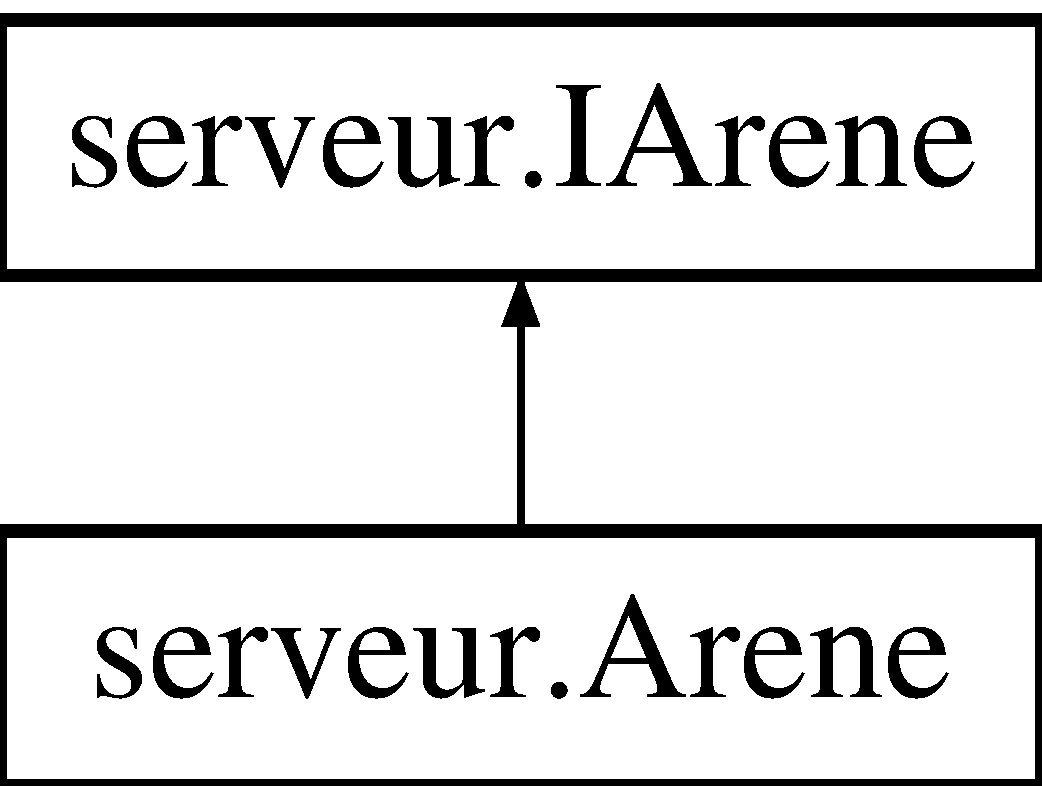
\includegraphics[height=2.000000cm]{classserveur_1_1_arene}
\end{center}
\end{figure}
\subsection*{Classes}
\begin{DoxyCompactItemize}
\item 
class \hyperlink{classserveur_1_1_arene_1_1_timeout_op}{Timeout\-Op}
\end{DoxyCompactItemize}
\subsection*{Public Member Functions}
\begin{DoxyCompactItemize}
\item 
\hyperlink{classserveur_1_1_arene_a5431d21bfdc858dbe31c6ec6b046aaca}{Arene} (int port)  throws Exception 
\item 
synchronized int \hyperlink{classserveur_1_1_arene_a88151079f2665d1973168e0cb266e3c7}{allocate\-Ref} ()  throws Remote\-Exception 
\item 
void \hyperlink{classserveur_1_1_arene_af37bb33255b051fa9236a62507eaf0ab}{run} ()
\item 
synchronized void \hyperlink{classserveur_1_1_arene_aa0f409b1844a97c1c413f04116cf863e}{connect} (\hyperlink{classinterface_graphique_1_1_vue_element}{Vue\-Element} s)  throws Remote\-Exception 
\item 
Array\-List$<$ \hyperlink{classinterface_graphique_1_1_vue_element}{Vue\-Element} $>$ \hyperlink{classserveur_1_1_arene_a83fb30e5a71d573d180997e60ab41304}{get\-World} ()  throws Remote\-Exception 
\item 
Hashtable$<$ Integer, \hyperlink{classinterface_graphique_1_1_vue_element}{Vue\-Element} $>$ \hyperlink{classserveur_1_1_arene_a1b8ef284b2fae162ba68884bfbe0160a}{voisins} (Point pos, int ref)  throws Remote\-Exception 
\item 
int \hyperlink{classserveur_1_1_arene_ad1bdc1a3aa97354caf2cb8c7d3f1a19b}{count\-Clients} ()
\item 
void \hyperlink{classserveur_1_1_arene_ae8331f4b3d827f4c93d4b1c08a0d9399}{interaction} (int ref, int ref2)  throws Remote\-Exception 
\item 
void \hyperlink{classserveur_1_1_arene_a930bd7387f12b44bcbfdc117fbd13672}{ramasser} (int ref, int ref2)  throws Remote\-Exception 
\item 
void \hyperlink{classserveur_1_1_arene_abbe9b4c0d7f5dcd711c702dc43c542f3}{supprimer\-Element} (Remote elem)
\end{DoxyCompactItemize}


\subsection{Detailed Description}
Le serveur ou se connectent les Consoles en R\-M\-I. En localhost pour l'instant 

\subsection{Constructor \& Destructor Documentation}
\hypertarget{classserveur_1_1_arene_a5431d21bfdc858dbe31c6ec6b046aaca}{\index{serveur\-::\-Arene@{serveur\-::\-Arene}!Arene@{Arene}}
\index{Arene@{Arene}!serveur::Arene@{serveur\-::\-Arene}}
\subsubsection[{Arene}]{\setlength{\rightskip}{0pt plus 5cm}serveur.\-Arene.\-Arene (
\begin{DoxyParamCaption}
\item[{int}]{port}
\end{DoxyParamCaption}
)  throws Exception }}\label{classserveur_1_1_arene_a5431d21bfdc858dbe31c6ec6b046aaca}
Constructeur 
\begin{DoxyParams}{Parameters}
{\em port} & le port de connexion \\
\hline
\end{DoxyParams}

\begin{DoxyExceptions}{Exceptions}
{\em Exception} & \\
\hline
\end{DoxyExceptions}


\subsection{Member Function Documentation}
\hypertarget{classserveur_1_1_arene_a88151079f2665d1973168e0cb266e3c7}{\index{serveur\-::\-Arene@{serveur\-::\-Arene}!allocate\-Ref@{allocate\-Ref}}
\index{allocate\-Ref@{allocate\-Ref}!serveur::Arene@{serveur\-::\-Arene}}
\subsubsection[{allocate\-Ref}]{\setlength{\rightskip}{0pt plus 5cm}synchronized int serveur.\-Arene.\-allocate\-Ref (
\begin{DoxyParamCaption}
{}
\end{DoxyParamCaption}
)  throws Remote\-Exception }}\label{classserveur_1_1_arene_a88151079f2665d1973168e0cb266e3c7}
Fournit une reference (entiere) pour un nouvel element dans l'arene, compte les elements la synchro permet de garantir l'acces e un seul thread a la fois au compteur++ \begin{DoxyReturn}{Returns}
reference (entiere) utilisee pour rmi, compter les elements 
\end{DoxyReturn}

\begin{DoxyExceptions}{Exceptions}
{\em Remote\-Exception} & \\
\hline
\end{DoxyExceptions}


Implements \hyperlink{interfaceserveur_1_1_i_arene_a6dc6a07ca0fdb5c2fd1ba53edd132298}{serveur.\-I\-Arene}.

\hypertarget{classserveur_1_1_arene_aa0f409b1844a97c1c413f04116cf863e}{\index{serveur\-::\-Arene@{serveur\-::\-Arene}!connect@{connect}}
\index{connect@{connect}!serveur::Arene@{serveur\-::\-Arene}}
\subsubsection[{connect}]{\setlength{\rightskip}{0pt plus 5cm}synchronized void serveur.\-Arene.\-connect (
\begin{DoxyParamCaption}
\item[{{\bf Vue\-Element}}]{s}
\end{DoxyParamCaption}
)  throws Remote\-Exception }}\label{classserveur_1_1_arene_aa0f409b1844a97c1c413f04116cf863e}
Associe (\char`\"{}connecte\char`\"{}) la representation d'un element en y associant un Remote, ajoute la representation d'un element dans l'arene
\begin{DoxyItemize}
\item la synchro permet de garantir qu'on ne fait pas de nouvelle connection pdt un tour de jeu 
\begin{DoxyParams}{Parameters}
{\em s} & vue (representation) de l'element \\
\hline
\end{DoxyParams}

\begin{DoxyExceptions}{Exceptions}
{\em Remote\-Exception} & \\
\hline
\end{DoxyExceptions}

\end{DoxyItemize}

Implements \hyperlink{interfaceserveur_1_1_i_arene_a5a051d16e51b7a0f368c4f89401a0293}{serveur.\-I\-Arene}.

\hypertarget{classserveur_1_1_arene_ad1bdc1a3aa97354caf2cb8c7d3f1a19b}{\index{serveur\-::\-Arene@{serveur\-::\-Arene}!count\-Clients@{count\-Clients}}
\index{count\-Clients@{count\-Clients}!serveur::Arene@{serveur\-::\-Arene}}
\subsubsection[{count\-Clients}]{\setlength{\rightskip}{0pt plus 5cm}int serveur.\-Arene.\-count\-Clients (
\begin{DoxyParamCaption}
{}
\end{DoxyParamCaption}
)}}\label{classserveur_1_1_arene_ad1bdc1a3aa97354caf2cb8c7d3f1a19b}
\begin{DoxyVerb}Renvoie le nombre de clients connectes
\end{DoxyVerb}
 \begin{DoxyReturn}{Returns}

\end{DoxyReturn}
\hypertarget{classserveur_1_1_arene_a83fb30e5a71d573d180997e60ab41304}{\index{serveur\-::\-Arene@{serveur\-::\-Arene}!get\-World@{get\-World}}
\index{get\-World@{get\-World}!serveur::Arene@{serveur\-::\-Arene}}
\subsubsection[{get\-World}]{\setlength{\rightskip}{0pt plus 5cm}Array\-List$<${\bf Vue\-Element}$>$ serveur.\-Arene.\-get\-World (
\begin{DoxyParamCaption}
{}
\end{DoxyParamCaption}
)  throws Remote\-Exception }}\label{classserveur_1_1_arene_a83fb30e5a71d573d180997e60ab41304}
\begin{DoxyVerb}appele par l'IHM pour afficher une representation de l'arene
via RMI, on envoie une copie (serialisee) du monde 
\end{DoxyVerb}
 
\begin{DoxyExceptions}{Exceptions}
{\em java.\-rmi.\-Remote\-Exception} & \\
\hline
\end{DoxyExceptions}


Implements \hyperlink{interfaceserveur_1_1_i_arene_ab7ea50f885f2cf28628d1c7ce2ca0159}{serveur.\-I\-Arene}.

\hypertarget{classserveur_1_1_arene_ae8331f4b3d827f4c93d4b1c08a0d9399}{\index{serveur\-::\-Arene@{serveur\-::\-Arene}!interaction@{interaction}}
\index{interaction@{interaction}!serveur::Arene@{serveur\-::\-Arene}}
\subsubsection[{interaction}]{\setlength{\rightskip}{0pt plus 5cm}void serveur.\-Arene.\-interaction (
\begin{DoxyParamCaption}
\item[{int}]{ref, }
\item[{int}]{ref2}
\end{DoxyParamCaption}
)  throws Remote\-Exception }}\label{classserveur_1_1_arene_ae8331f4b3d827f4c93d4b1c08a0d9399}
Methode d'interaction (combat) entre deux elements dont on a la reference 
\begin{DoxyParams}{Parameters}
{\em ref} & le premier element \\
\hline
{\em ref2} & le deuxieme element \\
\hline
\end{DoxyParams}

\begin{DoxyExceptions}{Exceptions}
{\em Remote\-Exception} & \\
\hline
\end{DoxyExceptions}


Implements \hyperlink{interfaceserveur_1_1_i_arene_aec66c3ded2467e80685b8cb4cf856cbc}{serveur.\-I\-Arene}.

\hypertarget{classserveur_1_1_arene_a930bd7387f12b44bcbfdc117fbd13672}{\index{serveur\-::\-Arene@{serveur\-::\-Arene}!ramasser@{ramasser}}
\index{ramasser@{ramasser}!serveur::Arene@{serveur\-::\-Arene}}
\subsubsection[{ramasser}]{\setlength{\rightskip}{0pt plus 5cm}void serveur.\-Arene.\-ramasser (
\begin{DoxyParamCaption}
\item[{int}]{ref, }
\item[{int}]{ref2}
\end{DoxyParamCaption}
)  throws Remote\-Exception }}\label{classserveur_1_1_arene_a930bd7387f12b44bcbfdc117fbd13672}
Ramassage de l'equipement par le comabattant 
\begin{DoxyParams}{Parameters}
{\em ref} & le combattant \\
\hline
{\em ref2} & l'objet a ramasser \\
\hline
\end{DoxyParams}

\begin{DoxyExceptions}{Exceptions}
{\em Remote\-Exception} & \\
\hline
\end{DoxyExceptions}


Implements \hyperlink{interfaceserveur_1_1_i_arene_adc0a9a0ec4b423e5b6a13a90091ead8c}{serveur.\-I\-Arene}.

\hypertarget{classserveur_1_1_arene_af37bb33255b051fa9236a62507eaf0ab}{\index{serveur\-::\-Arene@{serveur\-::\-Arene}!run@{run}}
\index{run@{run}!serveur::Arene@{serveur\-::\-Arene}}
\subsubsection[{run}]{\setlength{\rightskip}{0pt plus 5cm}void serveur.\-Arene.\-run (
\begin{DoxyParamCaption}
{}
\end{DoxyParamCaption}
)}}\label{classserveur_1_1_arene_af37bb33255b051fa9236a62507eaf0ab}
boucle principale du thread serveur \hypertarget{classserveur_1_1_arene_abbe9b4c0d7f5dcd711c702dc43c542f3}{\index{serveur\-::\-Arene@{serveur\-::\-Arene}!supprimer\-Element@{supprimer\-Element}}
\index{supprimer\-Element@{supprimer\-Element}!serveur::Arene@{serveur\-::\-Arene}}
\subsubsection[{supprimer\-Element}]{\setlength{\rightskip}{0pt plus 5cm}void serveur.\-Arene.\-supprimer\-Element (
\begin{DoxyParamCaption}
\item[{Remote}]{elem}
\end{DoxyParamCaption}
)}}\label{classserveur_1_1_arene_abbe9b4c0d7f5dcd711c702dc43c542f3}
Supprime un element de la liste des elements connectes au serveur 
\begin{DoxyParams}{Parameters}
{\em elem} & l'element a enlever \\
\hline
\end{DoxyParams}
\hypertarget{classserveur_1_1_arene_a1b8ef284b2fae162ba68884bfbe0160a}{\index{serveur\-::\-Arene@{serveur\-::\-Arene}!voisins@{voisins}}
\index{voisins@{voisins}!serveur::Arene@{serveur\-::\-Arene}}
\subsubsection[{voisins}]{\setlength{\rightskip}{0pt plus 5cm}Hashtable$<$Integer, {\bf Vue\-Element}$>$ serveur.\-Arene.\-voisins (
\begin{DoxyParamCaption}
\item[{Point}]{pos, }
\item[{int}]{ref}
\end{DoxyParamCaption}
)  throws Remote\-Exception }}\label{classserveur_1_1_arene_a1b8ef284b2fae162ba68884bfbe0160a}
\begin{DoxyVerb}Liste des reference des voisins et leurs coordonnees a partir d'une position
\end{DoxyVerb}
 
\begin{DoxyParams}{Parameters}
{\em pos} & \\
\hline
{\em ref} & \\
\hline
\end{DoxyParams}
\begin{DoxyReturn}{Returns}

\end{DoxyReturn}


Implements \hyperlink{interfaceserveur_1_1_i_arene_a47a37dbadfd6418b184e2c9f41faec01}{serveur.\-I\-Arene}.



The documentation for this class was generated from the following file\-:\begin{DoxyCompactItemize}
\item 
src/serveur/Arene.\-java\end{DoxyCompactItemize}

\hypertarget{classindividu_1_1combattant_1_1_barde}{\section{Référence de la classe individu.\-combattant.\-Barde}
\label{classindividu_1_1combattant_1_1_barde}\index{individu.\-combattant.\-Barde@{individu.\-combattant.\-Barde}}
}
Graphe d'héritage de individu.\-combattant.\-Barde\-:\begin{figure}[H]
\begin{center}
\leavevmode
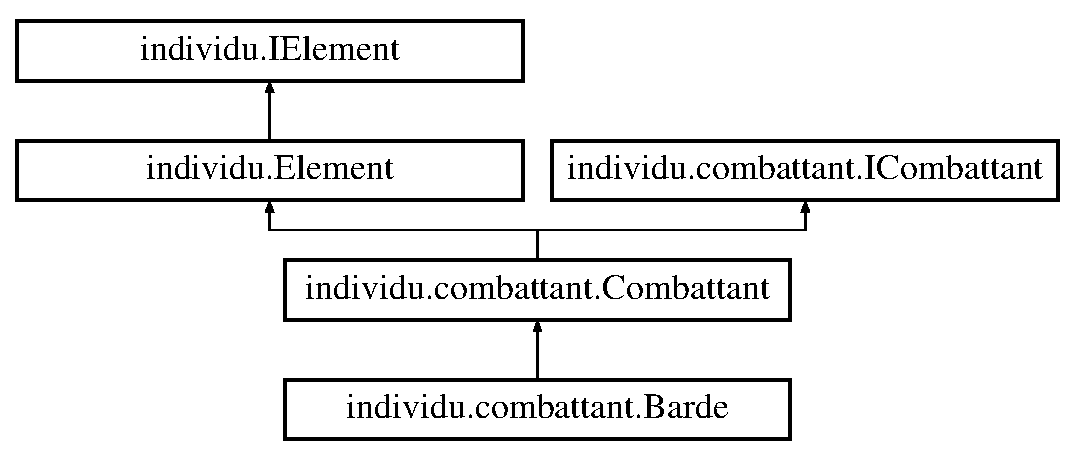
\includegraphics[height=4.000000cm]{classindividu_1_1combattant_1_1_barde}
\end{center}
\end{figure}
\subsection*{Fonctions membres publiques}
\begin{DoxyCompactItemize}
\item 
\hyperlink{classindividu_1_1combattant_1_1_barde_a19c43f6fb70721f159d1eb59ab5d58d3}{Barde} (String nom)
\end{DoxyCompactItemize}
\subsection*{Additional Inherited Members}


\subsection{Description détaillée}
Initialise un \hyperlink{classindividu_1_1combattant_1_1_combattant}{Combattant} avec les capacités d'un \hyperlink{classindividu_1_1combattant_1_1_barde}{Barde} 

\subsection{Documentation des constructeurs et destructeur}
\hypertarget{classindividu_1_1combattant_1_1_barde_a19c43f6fb70721f159d1eb59ab5d58d3}{\index{individu\-::combattant\-::\-Barde@{individu\-::combattant\-::\-Barde}!Barde@{Barde}}
\index{Barde@{Barde}!individu::combattant::Barde@{individu\-::combattant\-::\-Barde}}
\subsubsection[{Barde}]{\setlength{\rightskip}{0pt plus 5cm}individu.\-combattant.\-Barde.\-Barde (
\begin{DoxyParamCaption}
\item[{String}]{nom}
\end{DoxyParamCaption}
)}}\label{classindividu_1_1combattant_1_1_barde_a19c43f6fb70721f159d1eb59ab5d58d3}
Constructeur 
\begin{DoxyParams}{Paramètres}
{\em nom} & Le nom du \hyperlink{classindividu_1_1combattant_1_1_barde}{Barde} \\
\hline
\end{DoxyParams}


La documentation de cette classe a été générée à partir du fichier suivant \-:\begin{DoxyCompactItemize}
\item 
src/individu/combattant/Barde.\-java\end{DoxyCompactItemize}

\hypertarget{classindividu_1_1equipement_1_1_bottes}{\section{Référence de la classe individu.\-equipement.\-Bottes}
\label{classindividu_1_1equipement_1_1_bottes}\index{individu.\-equipement.\-Bottes@{individu.\-equipement.\-Bottes}}
}
Graphe d'héritage de individu.\-equipement.\-Bottes\-:\begin{figure}[H]
\begin{center}
\leavevmode
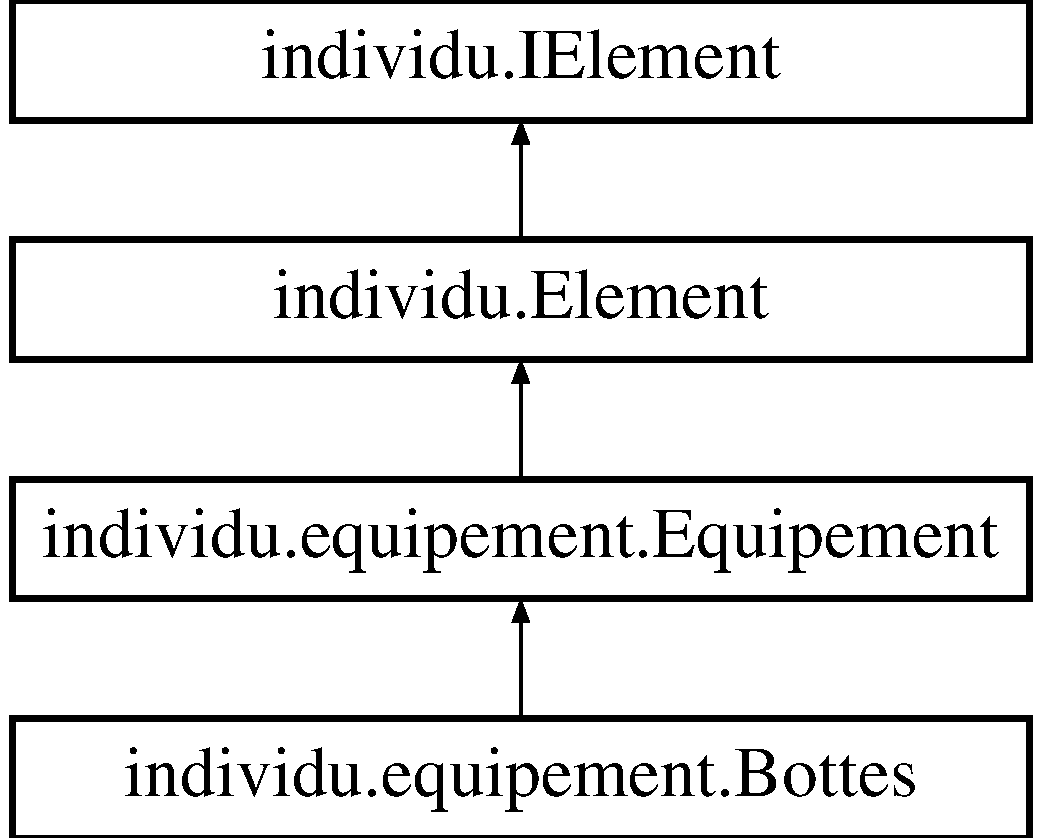
\includegraphics[height=4.000000cm]{classindividu_1_1equipement_1_1_bottes}
\end{center}
\end{figure}
\subsection*{Fonctions membres publiques}
\begin{DoxyCompactItemize}
\item 
\hypertarget{classindividu_1_1equipement_1_1_bottes_aa3558953e68ab09d53d2e99d620bd295}{{\bfseries Bottes} (String nom)}\label{classindividu_1_1equipement_1_1_bottes_aa3558953e68ab09d53d2e99d620bd295}

\end{DoxyCompactItemize}


\subsection{Description détaillée}
Initialise un équipement avec les capacités d'une botte 

La documentation de cette classe a été générée à partir du fichier suivant \-:\begin{DoxyCompactItemize}
\item 
src/individu/equipement/Bottes.\-java\end{DoxyCompactItemize}

\hypertarget{classindividu_1_1equipement_1_1_canne}{\section{Référence de la classe individu.\-equipement.\-Canne}
\label{classindividu_1_1equipement_1_1_canne}\index{individu.\-equipement.\-Canne@{individu.\-equipement.\-Canne}}
}
Graphe d'héritage de individu.\-equipement.\-Canne\-:\begin{figure}[H]
\begin{center}
\leavevmode
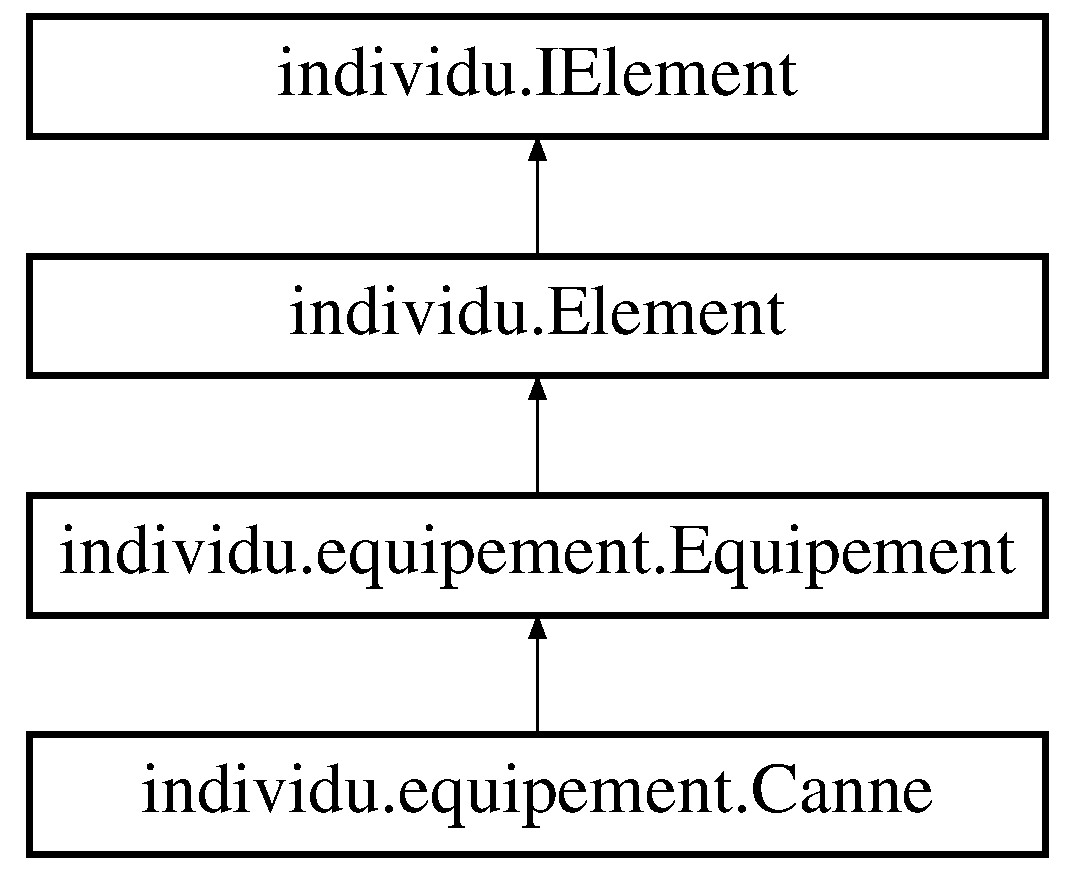
\includegraphics[height=4.000000cm]{classindividu_1_1equipement_1_1_canne}
\end{center}
\end{figure}
\subsection*{Fonctions membres publiques}
\begin{DoxyCompactItemize}
\item 
\hypertarget{classindividu_1_1equipement_1_1_canne_a0932a1ff5435367acb523544f221c78c}{{\bfseries Canne} (String nom)}\label{classindividu_1_1equipement_1_1_canne_a0932a1ff5435367acb523544f221c78c}

\end{DoxyCompactItemize}


\subsection{Description détaillée}
Initialise un équipement avec les capacités d'une canne 

La documentation de cette classe a été générée à partir du fichier suivant \-:\begin{DoxyCompactItemize}
\item 
src/individu/equipement/Canne.\-java\end{DoxyCompactItemize}

\hypertarget{classindividu_1_1combattant_1_1_capitaine}{\section{Référence de la classe individu.\-combattant.\-Capitaine}
\label{classindividu_1_1combattant_1_1_capitaine}\index{individu.\-combattant.\-Capitaine@{individu.\-combattant.\-Capitaine}}
}
Graphe d'héritage de individu.\-combattant.\-Capitaine\-:\begin{figure}[H]
\begin{center}
\leavevmode
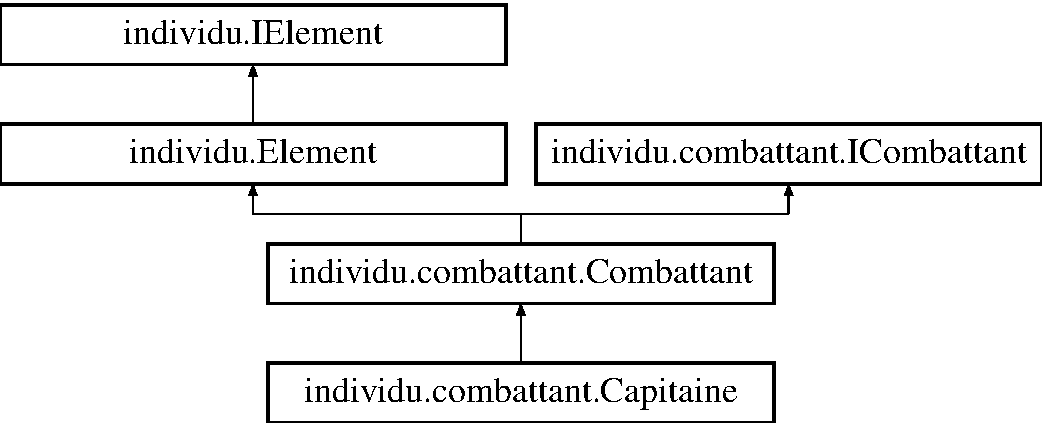
\includegraphics[height=4.000000cm]{classindividu_1_1combattant_1_1_capitaine}
\end{center}
\end{figure}
\subsection*{Fonctions membres publiques}
\begin{DoxyCompactItemize}
\item 
\hyperlink{classindividu_1_1combattant_1_1_capitaine_a27bb06c323e16dea4c2a2eabb4bc6b17}{Capitaine} (String nom)
\end{DoxyCompactItemize}
\subsection*{Additional Inherited Members}


\subsection{Description détaillée}
Initialise un \hyperlink{classindividu_1_1combattant_1_1_combattant}{Combattant} avec les capacités d'un \hyperlink{classindividu_1_1combattant_1_1_capitaine}{Capitaine} 

\subsection{Documentation des constructeurs et destructeur}
\hypertarget{classindividu_1_1combattant_1_1_capitaine_a27bb06c323e16dea4c2a2eabb4bc6b17}{\index{individu\-::combattant\-::\-Capitaine@{individu\-::combattant\-::\-Capitaine}!Capitaine@{Capitaine}}
\index{Capitaine@{Capitaine}!individu::combattant::Capitaine@{individu\-::combattant\-::\-Capitaine}}
\subsubsection[{Capitaine}]{\setlength{\rightskip}{0pt plus 5cm}individu.\-combattant.\-Capitaine.\-Capitaine (
\begin{DoxyParamCaption}
\item[{String}]{nom}
\end{DoxyParamCaption}
)}}\label{classindividu_1_1combattant_1_1_capitaine_a27bb06c323e16dea4c2a2eabb4bc6b17}
Constructeur 
\begin{DoxyParams}{Paramètres}
{\em nom} & Le nom du \hyperlink{classindividu_1_1combattant_1_1_capitaine}{Capitaine} \\
\hline
\end{DoxyParams}


La documentation de cette classe a été générée à partir du fichier suivant \-:\begin{DoxyCompactItemize}
\item 
src/individu/combattant/Capitaine.\-java\end{DoxyCompactItemize}

\hypertarget{classindividu_1_1equipement_1_1_chapeau_de_paille}{\section{Référence de la classe individu.\-equipement.\-Chapeau\-De\-Paille}
\label{classindividu_1_1equipement_1_1_chapeau_de_paille}\index{individu.\-equipement.\-Chapeau\-De\-Paille@{individu.\-equipement.\-Chapeau\-De\-Paille}}
}
Graphe d'héritage de individu.\-equipement.\-Chapeau\-De\-Paille\-:\begin{figure}[H]
\begin{center}
\leavevmode
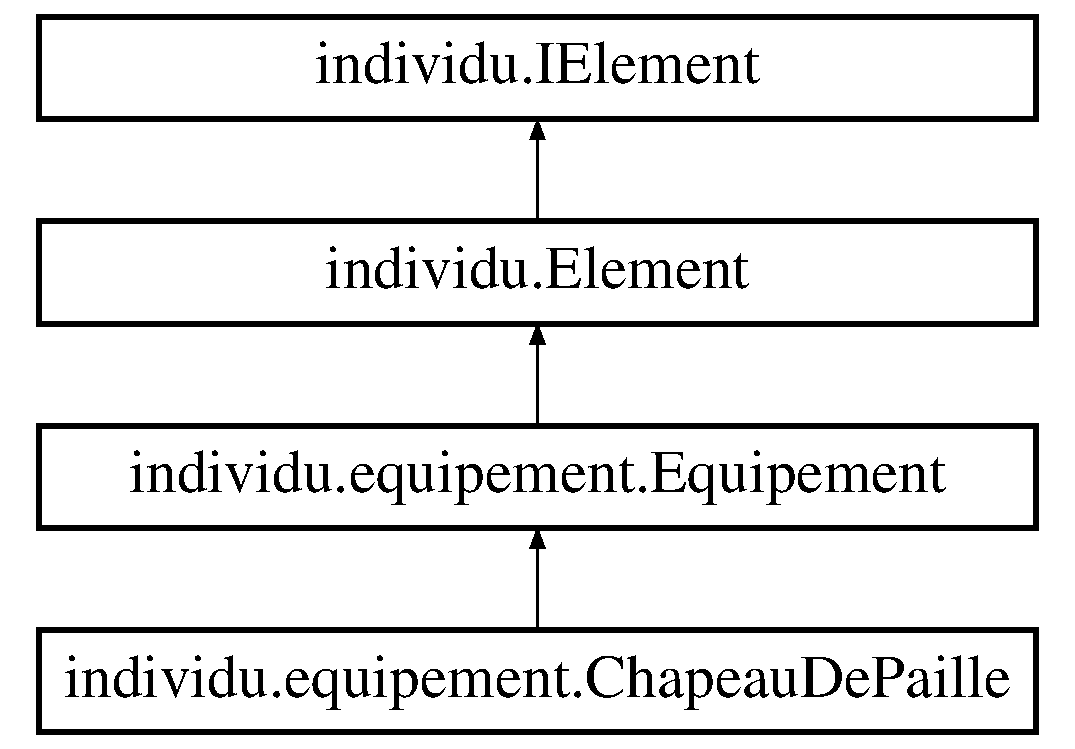
\includegraphics[height=4.000000cm]{classindividu_1_1equipement_1_1_chapeau_de_paille}
\end{center}
\end{figure}
\subsection*{Fonctions membres publiques}
\begin{DoxyCompactItemize}
\item 
\hypertarget{classindividu_1_1equipement_1_1_chapeau_de_paille_a51ef580b58d76d1642ef982fe78b90ab}{{\bfseries Chapeau\-De\-Paille} (String nom)}\label{classindividu_1_1equipement_1_1_chapeau_de_paille_a51ef580b58d76d1642ef982fe78b90ab}

\end{DoxyCompactItemize}


\subsection{Description détaillée}
Initialise un équipement avec les capacités d'un chapeau de paill 

La documentation de cette classe a été générée à partir du fichier suivant \-:\begin{DoxyCompactItemize}
\item 
src/individu/equipement/Chapeau\-De\-Paille.\-java\end{DoxyCompactItemize}

\hypertarget{classindividu_1_1combattant_1_1_combattant}{\section{Référence de la classe individu.\-combattant.\-Combattant}
\label{classindividu_1_1combattant_1_1_combattant}\index{individu.\-combattant.\-Combattant@{individu.\-combattant.\-Combattant}}
}
Graphe d'héritage de individu.\-combattant.\-Combattant\-:\begin{figure}[H]
\begin{center}
\leavevmode
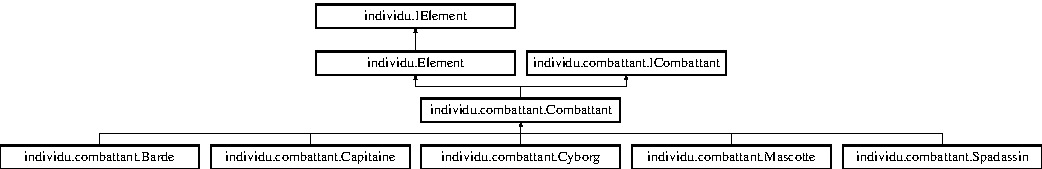
\includegraphics[height=2.274112cm]{classindividu_1_1combattant_1_1_combattant}
\end{center}
\end{figure}
\subsection*{Fonctions membres publiques}
\begin{DoxyCompactItemize}
\item 
\hyperlink{classindividu_1_1combattant_1_1_combattant_a4526e69f52d47876558f1c9cc10964db}{Combattant} (String nom)
\item 
\hyperlink{classindividu_1_1combattant_1_1_combattant_a9b9b0d6f38ad02317260adc9d08b612f}{Combattant} (String p\-Nom, final int p\-Vie, final int p\-Vitesse, final int p\-Defense, final int p\-Attaque, final int nb\-Objets\-Max)
\item 
\hyperlink{classindividu_1_1combattant_1_1_liste_equipements}{Liste\-Equipements} \hyperlink{classindividu_1_1combattant_1_1_combattant_a9d380a0a35876f99898fe7567cae32b9}{get\-Liste\-Equipement} ()
\item 
void \hyperlink{classindividu_1_1combattant_1_1_combattant_a2cf4b27020ffa07f6b6770dfd1654bc4}{gagner} (int s)
\item 
void \hyperlink{classindividu_1_1combattant_1_1_combattant_a46767973062954ee738e28856f1b6c6e}{perdre} (int s)
\item 
void \hyperlink{classindividu_1_1combattant_1_1_combattant_a7d56bc66f5eab04efdeeb748e29d1859}{ramasser} (int ref)
\item 
void \hyperlink{classindividu_1_1combattant_1_1_combattant_a127950f43fa0397daa5e23616bf6340c}{set\-Nb\-Objets} (final int p\-Nb\-Objets)
\item 
int \hyperlink{classindividu_1_1combattant_1_1_combattant_afe9afbb1b4d2b169054d1b3b31c1c362}{get\-Nb\-Objets} ()
\item 
void \hyperlink{classindividu_1_1combattant_1_1_combattant_a1d524c5ad7fc24f3210d7371363e5969}{set\-Argent} (int p\-Argent)
\item 
int \hyperlink{classindividu_1_1combattant_1_1_combattant_a1a6e4767d3b9bae8e913c427db5ffc64}{get\-Argent} ()
\item 
int \hyperlink{classindividu_1_1combattant_1_1_combattant_ad63c7efc58a08fbd0e76f43e0bbccd68}{get\-Attaque} ()
\item 
int \hyperlink{classindividu_1_1combattant_1_1_combattant_afda5816b9a5d7c44d24e3a870c779754}{get\-Defense} ()
\item 
int \hyperlink{classindividu_1_1combattant_1_1_combattant_ad04833b8576cf9933e2c6dd3e04269e8}{get\-Vitesse} ()
\item 
int \hyperlink{classindividu_1_1combattant_1_1_combattant_a08cc33106893423b5debcc5a8e7c1e34}{maj\-Duree\-Equip} ()
\end{DoxyCompactItemize}
\subsection*{Attributs protégés}
\begin{DoxyCompactItemize}
\item 
\hypertarget{classindividu_1_1combattant_1_1_combattant_acf5564d980faeef8eee5d28cce73556c}{final \hyperlink{classindividu_1_1combattant_1_1_liste_equipements}{Liste\-Equipements} \hyperlink{classindividu_1_1combattant_1_1_combattant_acf5564d980faeef8eee5d28cce73556c}{\-\_\-liste\-Equipement}}\label{classindividu_1_1combattant_1_1_combattant_acf5564d980faeef8eee5d28cce73556c}

\begin{DoxyCompactList}\small\item\em Liste contenant les équipements que possède le combattant. \end{DoxyCompactList}\end{DoxyCompactItemize}


\subsection{Description détaillée}
\hyperlink{classindividu_1_1combattant_1_1_combattant}{Combattant} générique \begin{DoxySeeAlso}{Voir également}
\hyperlink{classindividu_1_1combattant_1_1_liste_equipements}{Liste\-Equipements} 
\end{DoxySeeAlso}


\subsection{Documentation des constructeurs et destructeur}
\hypertarget{classindividu_1_1combattant_1_1_combattant_a4526e69f52d47876558f1c9cc10964db}{\index{individu\-::combattant\-::\-Combattant@{individu\-::combattant\-::\-Combattant}!Combattant@{Combattant}}
\index{Combattant@{Combattant}!individu::combattant::Combattant@{individu\-::combattant\-::\-Combattant}}
\subsubsection[{Combattant}]{\setlength{\rightskip}{0pt plus 5cm}individu.\-combattant.\-Combattant.\-Combattant (
\begin{DoxyParamCaption}
\item[{String}]{nom}
\end{DoxyParamCaption}
)}}\label{classindividu_1_1combattant_1_1_combattant_a4526e69f52d47876558f1c9cc10964db}
Constructeur initialiant toutes les capacités à 0 
\begin{DoxyParams}{Paramètres}
{\em nom} & Nom \\
\hline
\end{DoxyParams}
\hypertarget{classindividu_1_1combattant_1_1_combattant_a9b9b0d6f38ad02317260adc9d08b612f}{\index{individu\-::combattant\-::\-Combattant@{individu\-::combattant\-::\-Combattant}!Combattant@{Combattant}}
\index{Combattant@{Combattant}!individu::combattant::Combattant@{individu\-::combattant\-::\-Combattant}}
\subsubsection[{Combattant}]{\setlength{\rightskip}{0pt plus 5cm}individu.\-combattant.\-Combattant.\-Combattant (
\begin{DoxyParamCaption}
\item[{String}]{p\-Nom, }
\item[{final int}]{p\-Vie, }
\item[{final int}]{p\-Vitesse, }
\item[{final int}]{p\-Defense, }
\item[{final int}]{p\-Attaque, }
\item[{final int}]{nb\-Objets\-Max}
\end{DoxyParamCaption}
)}}\label{classindividu_1_1combattant_1_1_combattant_a9b9b0d6f38ad02317260adc9d08b612f}
Constructeur initialisant les valeurs du combattant 
\begin{DoxyParams}{Paramètres}
{\em p\-Nom} & Nom \\
\hline
{\em p\-Vie} & Vie \\
\hline
{\em p\-Vitesse} & Vitesse \\
\hline
{\em p\-Defense} & Défense \\
\hline
{\em p\-Attaque} & Attaque \\
\hline
{\em nb\-Objets\-Max} & Nombre maximum d'objets \\
\hline
\end{DoxyParams}


\subsection{Documentation des fonctions membres}
\hypertarget{classindividu_1_1combattant_1_1_combattant_a2cf4b27020ffa07f6b6770dfd1654bc4}{\index{individu\-::combattant\-::\-Combattant@{individu\-::combattant\-::\-Combattant}!gagner@{gagner}}
\index{gagner@{gagner}!individu::combattant::Combattant@{individu\-::combattant\-::\-Combattant}}
\subsubsection[{gagner}]{\setlength{\rightskip}{0pt plus 5cm}void individu.\-combattant.\-Combattant.\-gagner (
\begin{DoxyParamCaption}
\item[{int}]{s}
\end{DoxyParamCaption}
)}}\label{classindividu_1_1combattant_1_1_combattant_a2cf4b27020ffa07f6b6770dfd1654bc4}

\begin{DoxyParams}{Paramètres}
{\em s} & \\
\hline
\end{DoxyParams}


Implémente \hyperlink{interfaceindividu_1_1combattant_1_1_i_combattant_a8b656cde577f3346cee0f75450cbcb42}{individu.\-combattant.\-I\-Combattant}.

\hypertarget{classindividu_1_1combattant_1_1_combattant_a1a6e4767d3b9bae8e913c427db5ffc64}{\index{individu\-::combattant\-::\-Combattant@{individu\-::combattant\-::\-Combattant}!get\-Argent@{get\-Argent}}
\index{get\-Argent@{get\-Argent}!individu::combattant::Combattant@{individu\-::combattant\-::\-Combattant}}
\subsubsection[{get\-Argent}]{\setlength{\rightskip}{0pt plus 5cm}int individu.\-combattant.\-Combattant.\-get\-Argent (
\begin{DoxyParamCaption}
{}
\end{DoxyParamCaption}
)}}\label{classindividu_1_1combattant_1_1_combattant_a1a6e4767d3b9bae8e913c427db5ffc64}
Retourne l'argent du combattant \begin{DoxyReturn}{Renvoie}
L'argent 
\end{DoxyReturn}


Implémente \hyperlink{interfaceindividu_1_1combattant_1_1_i_combattant_a820ac1fbe763b07ae4300a58f6fc0463}{individu.\-combattant.\-I\-Combattant}.

\hypertarget{classindividu_1_1combattant_1_1_combattant_ad63c7efc58a08fbd0e76f43e0bbccd68}{\index{individu\-::combattant\-::\-Combattant@{individu\-::combattant\-::\-Combattant}!get\-Attaque@{get\-Attaque}}
\index{get\-Attaque@{get\-Attaque}!individu::combattant::Combattant@{individu\-::combattant\-::\-Combattant}}
\subsubsection[{get\-Attaque}]{\setlength{\rightskip}{0pt plus 5cm}int individu.\-combattant.\-Combattant.\-get\-Attaque (
\begin{DoxyParamCaption}
{}
\end{DoxyParamCaption}
)}}\label{classindividu_1_1combattant_1_1_combattant_ad63c7efc58a08fbd0e76f43e0bbccd68}
Retourne la capacité d'attaque du combattant en prenant en compte son équipement \begin{DoxyReturn}{Renvoie}
La capacité d'attaque 
\end{DoxyReturn}


Réimplémentée à partir de \hyperlink{classindividu_1_1_element_a911dfb782eeaf4d472189ee9f89e9c78}{individu.\-Element}.

\hypertarget{classindividu_1_1combattant_1_1_combattant_afda5816b9a5d7c44d24e3a870c779754}{\index{individu\-::combattant\-::\-Combattant@{individu\-::combattant\-::\-Combattant}!get\-Defense@{get\-Defense}}
\index{get\-Defense@{get\-Defense}!individu::combattant::Combattant@{individu\-::combattant\-::\-Combattant}}
\subsubsection[{get\-Defense}]{\setlength{\rightskip}{0pt plus 5cm}int individu.\-combattant.\-Combattant.\-get\-Defense (
\begin{DoxyParamCaption}
{}
\end{DoxyParamCaption}
)}}\label{classindividu_1_1combattant_1_1_combattant_afda5816b9a5d7c44d24e3a870c779754}
Retourne la défense du combattant en prenant en compte son équipement \begin{DoxyReturn}{Renvoie}
La défense 
\end{DoxyReturn}


Réimplémentée à partir de \hyperlink{classindividu_1_1_element_a5dfa6bd163796694365cbd3f5aa1548d}{individu.\-Element}.

\hypertarget{classindividu_1_1combattant_1_1_combattant_a9d380a0a35876f99898fe7567cae32b9}{\index{individu\-::combattant\-::\-Combattant@{individu\-::combattant\-::\-Combattant}!get\-Liste\-Equipement@{get\-Liste\-Equipement}}
\index{get\-Liste\-Equipement@{get\-Liste\-Equipement}!individu::combattant::Combattant@{individu\-::combattant\-::\-Combattant}}
\subsubsection[{get\-Liste\-Equipement}]{\setlength{\rightskip}{0pt plus 5cm}{\bf Liste\-Equipements} individu.\-combattant.\-Combattant.\-get\-Liste\-Equipement (
\begin{DoxyParamCaption}
{}
\end{DoxyParamCaption}
)}}\label{classindividu_1_1combattant_1_1_combattant_a9d380a0a35876f99898fe7567cae32b9}
\begin{DoxyReturn}{Renvoie}

\end{DoxyReturn}
\hypertarget{classindividu_1_1combattant_1_1_combattant_afe9afbb1b4d2b169054d1b3b31c1c362}{\index{individu\-::combattant\-::\-Combattant@{individu\-::combattant\-::\-Combattant}!get\-Nb\-Objets@{get\-Nb\-Objets}}
\index{get\-Nb\-Objets@{get\-Nb\-Objets}!individu::combattant::Combattant@{individu\-::combattant\-::\-Combattant}}
\subsubsection[{get\-Nb\-Objets}]{\setlength{\rightskip}{0pt plus 5cm}int individu.\-combattant.\-Combattant.\-get\-Nb\-Objets (
\begin{DoxyParamCaption}
{}
\end{DoxyParamCaption}
)}}\label{classindividu_1_1combattant_1_1_combattant_afe9afbb1b4d2b169054d1b3b31c1c362}
Retourne le nombre d'objets maximum du combattant \begin{DoxyReturn}{Renvoie}
Le nombre d'objet 
\end{DoxyReturn}


Implémente \hyperlink{interfaceindividu_1_1combattant_1_1_i_combattant_abf39b472bad06221d901d2d143ee5c91}{individu.\-combattant.\-I\-Combattant}.

\hypertarget{classindividu_1_1combattant_1_1_combattant_ad04833b8576cf9933e2c6dd3e04269e8}{\index{individu\-::combattant\-::\-Combattant@{individu\-::combattant\-::\-Combattant}!get\-Vitesse@{get\-Vitesse}}
\index{get\-Vitesse@{get\-Vitesse}!individu::combattant::Combattant@{individu\-::combattant\-::\-Combattant}}
\subsubsection[{get\-Vitesse}]{\setlength{\rightskip}{0pt plus 5cm}int individu.\-combattant.\-Combattant.\-get\-Vitesse (
\begin{DoxyParamCaption}
{}
\end{DoxyParamCaption}
)}}\label{classindividu_1_1combattant_1_1_combattant_ad04833b8576cf9933e2c6dd3e04269e8}
Retourne la vitesse d'esquive en prenant en compte son équipement \begin{DoxyReturn}{Renvoie}
La vitesse 
\end{DoxyReturn}


Réimplémentée à partir de \hyperlink{classindividu_1_1_element_a4ccd4fbf75bf5f1020aba19b9c78d43d}{individu.\-Element}.

\hypertarget{classindividu_1_1combattant_1_1_combattant_a08cc33106893423b5debcc5a8e7c1e34}{\index{individu\-::combattant\-::\-Combattant@{individu\-::combattant\-::\-Combattant}!maj\-Duree\-Equip@{maj\-Duree\-Equip}}
\index{maj\-Duree\-Equip@{maj\-Duree\-Equip}!individu::combattant::Combattant@{individu\-::combattant\-::\-Combattant}}
\subsubsection[{maj\-Duree\-Equip}]{\setlength{\rightskip}{0pt plus 5cm}int individu.\-combattant.\-Combattant.\-maj\-Duree\-Equip (
\begin{DoxyParamCaption}
{}
\end{DoxyParamCaption}
)}}\label{classindividu_1_1combattant_1_1_combattant_a08cc33106893423b5debcc5a8e7c1e34}
Met à jour la durée de vie de l'équipement du combattant \begin{DoxyReturn}{Renvoie}
La nouvelle durée 
\end{DoxyReturn}
\hypertarget{classindividu_1_1combattant_1_1_combattant_a46767973062954ee738e28856f1b6c6e}{\index{individu\-::combattant\-::\-Combattant@{individu\-::combattant\-::\-Combattant}!perdre@{perdre}}
\index{perdre@{perdre}!individu::combattant::Combattant@{individu\-::combattant\-::\-Combattant}}
\subsubsection[{perdre}]{\setlength{\rightskip}{0pt plus 5cm}void individu.\-combattant.\-Combattant.\-perdre (
\begin{DoxyParamCaption}
\item[{int}]{s}
\end{DoxyParamCaption}
)}}\label{classindividu_1_1combattant_1_1_combattant_a46767973062954ee738e28856f1b6c6e}

\begin{DoxyParams}{Paramètres}
{\em s} & \\
\hline
\end{DoxyParams}


Implémente \hyperlink{interfaceindividu_1_1combattant_1_1_i_combattant_a762a6a778b7a09fa32564e6dd9e0aa46}{individu.\-combattant.\-I\-Combattant}.

\hypertarget{classindividu_1_1combattant_1_1_combattant_a7d56bc66f5eab04efdeeb748e29d1859}{\index{individu\-::combattant\-::\-Combattant@{individu\-::combattant\-::\-Combattant}!ramasser@{ramasser}}
\index{ramasser@{ramasser}!individu::combattant::Combattant@{individu\-::combattant\-::\-Combattant}}
\subsubsection[{ramasser}]{\setlength{\rightskip}{0pt plus 5cm}void individu.\-combattant.\-Combattant.\-ramasser (
\begin{DoxyParamCaption}
\item[{int}]{ref}
\end{DoxyParamCaption}
)}}\label{classindividu_1_1combattant_1_1_combattant_a7d56bc66f5eab04efdeeb748e29d1859}

\begin{DoxyParams}{Paramètres}
{\em ref} & \\
\hline
\end{DoxyParams}


Implémente \hyperlink{interfaceindividu_1_1combattant_1_1_i_combattant_a48e6090fc4b67a81a8028477ea6b15e7}{individu.\-combattant.\-I\-Combattant}.

\hypertarget{classindividu_1_1combattant_1_1_combattant_a1d524c5ad7fc24f3210d7371363e5969}{\index{individu\-::combattant\-::\-Combattant@{individu\-::combattant\-::\-Combattant}!set\-Argent@{set\-Argent}}
\index{set\-Argent@{set\-Argent}!individu::combattant::Combattant@{individu\-::combattant\-::\-Combattant}}
\subsubsection[{set\-Argent}]{\setlength{\rightskip}{0pt plus 5cm}void individu.\-combattant.\-Combattant.\-set\-Argent (
\begin{DoxyParamCaption}
\item[{int}]{p\-Argent}
\end{DoxyParamCaption}
)}}\label{classindividu_1_1combattant_1_1_combattant_a1d524c5ad7fc24f3210d7371363e5969}
Réinitialie l'argent du combattant 
\begin{DoxyParams}{Paramètres}
{\em p\-Argent} & La nouvelle valeure \\
\hline
\end{DoxyParams}
\hypertarget{classindividu_1_1combattant_1_1_combattant_a127950f43fa0397daa5e23616bf6340c}{\index{individu\-::combattant\-::\-Combattant@{individu\-::combattant\-::\-Combattant}!set\-Nb\-Objets@{set\-Nb\-Objets}}
\index{set\-Nb\-Objets@{set\-Nb\-Objets}!individu::combattant::Combattant@{individu\-::combattant\-::\-Combattant}}
\subsubsection[{set\-Nb\-Objets}]{\setlength{\rightskip}{0pt plus 5cm}void individu.\-combattant.\-Combattant.\-set\-Nb\-Objets (
\begin{DoxyParamCaption}
\item[{final int}]{p\-Nb\-Objets}
\end{DoxyParamCaption}
)}}\label{classindividu_1_1combattant_1_1_combattant_a127950f43fa0397daa5e23616bf6340c}
Réinitialise le nombre d'objets maximum 
\begin{DoxyParams}{Paramètres}
{\em p\-Nb\-Objets} & Nouveau nombre d'objet \\
\hline
\end{DoxyParams}


Implémente \hyperlink{interfaceindividu_1_1combattant_1_1_i_combattant_aca0de8e3df27d07ceb216e022c403cc6}{individu.\-combattant.\-I\-Combattant}.



La documentation de cette classe a été générée à partir du fichier suivant \-:\begin{DoxyCompactItemize}
\item 
src/individu/combattant/Combattant.\-java\end{DoxyCompactItemize}

\hypertarget{classcontrole_1_1_console}{\section{controle.\-Console Class Reference}
\label{classcontrole_1_1_console}\index{controle.\-Console@{controle.\-Console}}
}
Inheritance diagram for controle.\-Console\-:\begin{figure}[H]
\begin{center}
\leavevmode
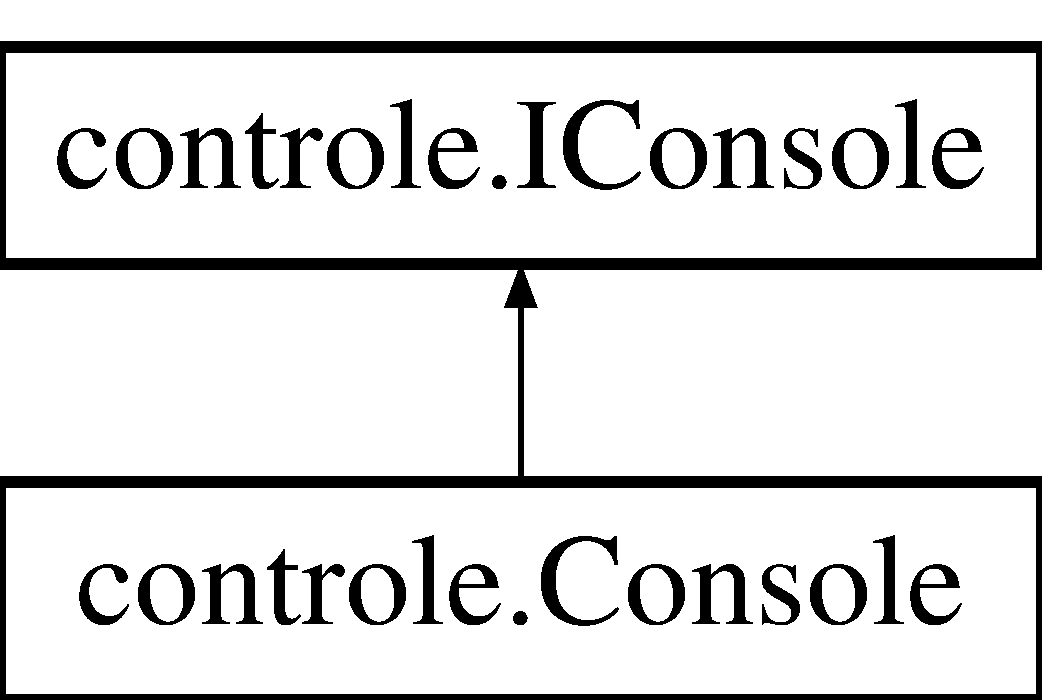
\includegraphics[height=2.000000cm]{classcontrole_1_1_console}
\end{center}
\end{figure}
\subsection*{Public Member Functions}
\begin{DoxyCompactItemize}
\item 
\hyperlink{classcontrole_1_1_console_a35af1c179b641b9afee8647567668b58}{Console} (\hyperlink{classindividu_1_1_element}{Element} elem, int dx, int dy)  throws Remote\-Exception 
\item 
void \hyperlink{classcontrole_1_1_console_a152371882b9665bde857d76438d70d02}{run} ()  throws Remote\-Exception 
\item 
void \hyperlink{classcontrole_1_1_console_aec0965feae069d1376b6ab0996767be8}{se\-Diriger\-Vers} (int ref)
\item 
\hyperlink{classinterface_graphique_1_1_vue_element}{Vue\-Element} \hyperlink{classcontrole_1_1_console_a67a69e366628189229f757915169de2e}{update} ()  throws Remote\-Exception 
\item 
void \hyperlink{classcontrole_1_1_console_a59029e1a06e0276d7ef75ba69bd0c16b}{shut\-Down} (String cause)  throws Remote\-Exception 
\item 
\hyperlink{classindividu_1_1_element}{Element} \hyperlink{classcontrole_1_1_console_abfbaec728b66178c064fd56ded8ece87}{get\-Element} ()  throws Remote\-Exception 
\item 
\hyperlink{classinterface_graphique_1_1_vue_element}{Vue\-Element} \hyperlink{classcontrole_1_1_console_ad1573e5279879abd84a460ffb080fdf3}{get\-Vue\-Element} ()  throws Remote\-Exception 
\item 
void \hyperlink{classcontrole_1_1_console_ad7157537fa92a47ed06563586dba5e2d}{parler} (String s)  throws Remote\-Exception 
\item 
void \hyperlink{classcontrole_1_1_console_a046b6d6c18e8bbecad7a4ff4e2c35a8f}{perdre\-Vie} (int vie\-Perdue)  throws Remote\-Exception 
\item 
void \hyperlink{classcontrole_1_1_console_aaa5374f35b30f5c232aac22041801c38}{ramasser\-Objet} (\hyperlink{interfacecontrole_1_1_i_console}{I\-Console} objet)  throws Remote\-Exception 
\item 
String \hyperlink{classcontrole_1_1_console_a750f2122aee6e608375f999cdfa5f43b}{afficher} ()  throws Remote\-Exception
\item 
void \hyperlink{classcontrole_1_1_console_aae7e697a8bc845c11c1430c08edd6b8c}{ajouter\-Connu} (int ref)  throws Remote\-Exception 
\end{DoxyCompactItemize}


\subsection{Detailed Description}
Se connecte au serveur avec un Element et sa Vue\-Element. \char`\"{}run\char`\"{} permet a l'Element/\-Vue\-Element de se deplacer 

\subsection{Constructor \& Destructor Documentation}
\hypertarget{classcontrole_1_1_console_a35af1c179b641b9afee8647567668b58}{\index{controle\-::\-Console@{controle\-::\-Console}!Console@{Console}}
\index{Console@{Console}!controle::Console@{controle\-::\-Console}}
\subsubsection[{Console}]{\setlength{\rightskip}{0pt plus 5cm}controle.\-Console.\-Console (
\begin{DoxyParamCaption}
\item[{{\bf Element}}]{elem, }
\item[{int}]{dx, }
\item[{int}]{dy}
\end{DoxyParamCaption}
)  throws Remote\-Exception }}\label{classcontrole_1_1_console_a35af1c179b641b9afee8647567668b58}
Constructeur 
\begin{DoxyParams}{Parameters}
{\em elem} & l'element pour lequel le controleur est cree \\
\hline
{\em dx} & la position initiale de l'element sur l'ordonnee (interface graphique) \\
\hline
{\em dy} & la position initiale de l'element sur l'abscisse (interface graphique) \\
\hline
\end{DoxyParams}

\begin{DoxyExceptions}{Exceptions}
{\em Remote\-Exception} & \\
\hline
\end{DoxyExceptions}


\subsection{Member Function Documentation}
\hypertarget{classcontrole_1_1_console_a750f2122aee6e608375f999cdfa5f43b}{\index{controle\-::\-Console@{controle\-::\-Console}!afficher@{afficher}}
\index{afficher@{afficher}!controle::Console@{controle\-::\-Console}}
\subsubsection[{afficher}]{\setlength{\rightskip}{0pt plus 5cm}String controle.\-Console.\-afficher (
\begin{DoxyParamCaption}
{}
\end{DoxyParamCaption}
)  throws Remote\-Exception}}\label{classcontrole_1_1_console_a750f2122aee6e608375f999cdfa5f43b}
\begin{DoxyVerb}Renvoie l'etat de l'element a afficher sur l'interface graphique
\end{DoxyVerb}
 \begin{DoxyReturn}{Returns}

\end{DoxyReturn}

\begin{DoxyExceptions}{Exceptions}
{\em Remote\-Exception} & \\
\hline
\end{DoxyExceptions}


Implements \hyperlink{interfacecontrole_1_1_i_console_a6166aa60251707f3c095e8e197a88dac}{controle.\-I\-Console}.

\hypertarget{classcontrole_1_1_console_aae7e697a8bc845c11c1430c08edd6b8c}{\index{controle\-::\-Console@{controle\-::\-Console}!ajouter\-Connu@{ajouter\-Connu}}
\index{ajouter\-Connu@{ajouter\-Connu}!controle::Console@{controle\-::\-Console}}
\subsubsection[{ajouter\-Connu}]{\setlength{\rightskip}{0pt plus 5cm}void controle.\-Console.\-ajouter\-Connu (
\begin{DoxyParamCaption}
\item[{int}]{ref}
\end{DoxyParamCaption}
)  throws Remote\-Exception }}\label{classcontrole_1_1_console_aae7e697a8bc845c11c1430c08edd6b8c}
Ajout l'element dans la liste des elements connus (combattants et equipements) 
\begin{DoxyParams}{Parameters}
{\em ref} & l'element a ajouter \\
\hline
\end{DoxyParams}


Implements \hyperlink{interfacecontrole_1_1_i_console_ac0aefd004a73641f8ba6ef57266c0508}{controle.\-I\-Console}.

\hypertarget{classcontrole_1_1_console_abfbaec728b66178c064fd56ded8ece87}{\index{controle\-::\-Console@{controle\-::\-Console}!get\-Element@{get\-Element}}
\index{get\-Element@{get\-Element}!controle::Console@{controle\-::\-Console}}
\subsubsection[{get\-Element}]{\setlength{\rightskip}{0pt plus 5cm}{\bf Element} controle.\-Console.\-get\-Element (
\begin{DoxyParamCaption}
{}
\end{DoxyParamCaption}
)  throws Remote\-Exception }}\label{classcontrole_1_1_console_abfbaec728b66178c064fd56ded8ece87}
\begin{DoxyVerb}Renvoie l'element associe a la console
\end{DoxyVerb}
 \begin{DoxyReturn}{Returns}

\end{DoxyReturn}

\begin{DoxyExceptions}{Exceptions}
{\em Remote\-Exception} & \\
\hline
\end{DoxyExceptions}


Implements \hyperlink{interfacecontrole_1_1_i_console_a0cde95415052505230b482a2b5fed5fd}{controle.\-I\-Console}.

\hypertarget{classcontrole_1_1_console_ad1573e5279879abd84a460ffb080fdf3}{\index{controle\-::\-Console@{controle\-::\-Console}!get\-Vue\-Element@{get\-Vue\-Element}}
\index{get\-Vue\-Element@{get\-Vue\-Element}!controle::Console@{controle\-::\-Console}}
\subsubsection[{get\-Vue\-Element}]{\setlength{\rightskip}{0pt plus 5cm}{\bf Vue\-Element} controle.\-Console.\-get\-Vue\-Element (
\begin{DoxyParamCaption}
{}
\end{DoxyParamCaption}
)  throws Remote\-Exception }}\label{classcontrole_1_1_console_ad1573e5279879abd84a460ffb080fdf3}
\begin{DoxyVerb}Renvoie la vue de l'element associe a la console
\end{DoxyVerb}
 \begin{DoxyReturn}{Returns}

\end{DoxyReturn}

\begin{DoxyExceptions}{Exceptions}
{\em Remote\-Exception} & \\
\hline
\end{DoxyExceptions}


Implements \hyperlink{interfacecontrole_1_1_i_console_a5fc11711131f9a99768d36bffc695535}{controle.\-I\-Console}.

\hypertarget{classcontrole_1_1_console_ad7157537fa92a47ed06563586dba5e2d}{\index{controle\-::\-Console@{controle\-::\-Console}!parler@{parler}}
\index{parler@{parler}!controle::Console@{controle\-::\-Console}}
\subsubsection[{parler}]{\setlength{\rightskip}{0pt plus 5cm}void controle.\-Console.\-parler (
\begin{DoxyParamCaption}
\item[{String}]{message}
\end{DoxyParamCaption}
)  throws Remote\-Exception }}\label{classcontrole_1_1_console_ad7157537fa92a47ed06563586dba5e2d}
L'element associe a la vue met a jour sa phrase 
\begin{DoxyParams}{Parameters}
{\em message} & la nouvelle phrase a communique \\
\hline
\end{DoxyParams}

\begin{DoxyExceptions}{Exceptions}
{\em Remote\-Exception} & \\
\hline
\end{DoxyExceptions}


Implements \hyperlink{interfacecontrole_1_1_i_console_ab200b6a49e88391691be5df49cfa36f2}{controle.\-I\-Console}.

\hypertarget{classcontrole_1_1_console_a046b6d6c18e8bbecad7a4ff4e2c35a8f}{\index{controle\-::\-Console@{controle\-::\-Console}!perdre\-Vie@{perdre\-Vie}}
\index{perdre\-Vie@{perdre\-Vie}!controle::Console@{controle\-::\-Console}}
\subsubsection[{perdre\-Vie}]{\setlength{\rightskip}{0pt plus 5cm}void controle.\-Console.\-perdre\-Vie (
\begin{DoxyParamCaption}
\item[{int}]{vie\-Perdue}
\end{DoxyParamCaption}
)  throws Remote\-Exception }}\label{classcontrole_1_1_console_a046b6d6c18e8bbecad7a4ff4e2c35a8f}
L'element associe au controleur perd des vies 
\begin{DoxyParams}{Parameters}
{\em vie\-Perdue} & le nombre de vies que l'element perd \\
\hline
\end{DoxyParams}

\begin{DoxyExceptions}{Exceptions}
{\em Remote\-Exception} & \\
\hline
\end{DoxyExceptions}


Implements \hyperlink{interfacecontrole_1_1_i_console_ace6ee762b3f067e26f478066a9c1283f}{controle.\-I\-Console}.

\hypertarget{classcontrole_1_1_console_aaa5374f35b30f5c232aac22041801c38}{\index{controle\-::\-Console@{controle\-::\-Console}!ramasser\-Objet@{ramasser\-Objet}}
\index{ramasser\-Objet@{ramasser\-Objet}!controle::Console@{controle\-::\-Console}}
\subsubsection[{ramasser\-Objet}]{\setlength{\rightskip}{0pt plus 5cm}void controle.\-Console.\-ramasser\-Objet (
\begin{DoxyParamCaption}
\item[{{\bf I\-Console}}]{objet}
\end{DoxyParamCaption}
)  throws Remote\-Exception }}\label{classcontrole_1_1_console_aaa5374f35b30f5c232aac22041801c38}
L'element associe au controleur ramasse un objet 
\begin{DoxyParams}{Parameters}
{\em objet} & l'objet ramasse par l'element \\
\hline
\end{DoxyParams}

\begin{DoxyExceptions}{Exceptions}
{\em Remote\-Exception} & \\
\hline
\end{DoxyExceptions}


Implements \hyperlink{interfacecontrole_1_1_i_console_a90d8826ee94075bc55a52779a0257b85}{controle.\-I\-Console}.

\hypertarget{classcontrole_1_1_console_a152371882b9665bde857d76438d70d02}{\index{controle\-::\-Console@{controle\-::\-Console}!run@{run}}
\index{run@{run}!controle::Console@{controle\-::\-Console}}
\subsubsection[{run}]{\setlength{\rightskip}{0pt plus 5cm}void controle.\-Console.\-run (
\begin{DoxyParamCaption}
{}
\end{DoxyParamCaption}
)  throws Remote\-Exception }}\label{classcontrole_1_1_console_a152371882b9665bde857d76438d70d02}
Permet au serveur de faire \char`\"{}jouer\char`\"{} un tour a l'element. Calcule ses voisins (donnes par le serveur), cherche le plus proche, s'il est a proximite, lance l'interaction sinon se dirige vers lui (s'il existe un plus proche) Cette methode est execute chaque seconde 

Implements \hyperlink{interfacecontrole_1_1_i_console_afb2a3e548fe438ac7af6bc429fc84132}{controle.\-I\-Console}.

\hypertarget{classcontrole_1_1_console_aec0965feae069d1376b6ab0996767be8}{\index{controle\-::\-Console@{controle\-::\-Console}!se\-Diriger\-Vers@{se\-Diriger\-Vers}}
\index{se\-Diriger\-Vers@{se\-Diriger\-Vers}!controle::Console@{controle\-::\-Console}}
\subsubsection[{se\-Diriger\-Vers}]{\setlength{\rightskip}{0pt plus 5cm}void controle.\-Console.\-se\-Diriger\-Vers (
\begin{DoxyParamCaption}
\item[{int}]{ref}
\end{DoxyParamCaption}
)}}\label{classcontrole_1_1_console_aec0965feae069d1376b6ab0996767be8}
Deplace ce sujet d'une case en direction du sujet dont la reference est donnee en parametre 
\begin{DoxyParams}{Parameters}
{\em ref} & la reference de l'element cible \\
\hline
\end{DoxyParams}
\hypertarget{classcontrole_1_1_console_a59029e1a06e0276d7ef75ba69bd0c16b}{\index{controle\-::\-Console@{controle\-::\-Console}!shut\-Down@{shut\-Down}}
\index{shut\-Down@{shut\-Down}!controle::Console@{controle\-::\-Console}}
\subsubsection[{shut\-Down}]{\setlength{\rightskip}{0pt plus 5cm}void controle.\-Console.\-shut\-Down (
\begin{DoxyParamCaption}
\item[{String}]{cause}
\end{DoxyParamCaption}
)  throws Remote\-Exception }}\label{classcontrole_1_1_console_a59029e1a06e0276d7ef75ba69bd0c16b}
Deconnexion du controleur du serveur 
\begin{DoxyParams}{Parameters}
{\em cause} & le message a afficher comme cause de la deconnexion \\
\hline
\end{DoxyParams}


Implements \hyperlink{interfacecontrole_1_1_i_console_a77e327568514ec7eed8161c6b73e4d9a}{controle.\-I\-Console}.

\hypertarget{classcontrole_1_1_console_a67a69e366628189229f757915169de2e}{\index{controle\-::\-Console@{controle\-::\-Console}!update@{update}}
\index{update@{update}!controle::Console@{controle\-::\-Console}}
\subsubsection[{update}]{\setlength{\rightskip}{0pt plus 5cm}{\bf Vue\-Element} controle.\-Console.\-update (
\begin{DoxyParamCaption}
{}
\end{DoxyParamCaption}
)  throws Remote\-Exception }}\label{classcontrole_1_1_console_a67a69e366628189229f757915169de2e}
Appelle par le serveur pour faire la M\-A\-J du sujet 

Implements \hyperlink{interfacecontrole_1_1_i_console_ab6728a4bf807f04e5d13bfd452a69bc2}{controle.\-I\-Console}.



The documentation for this class was generated from the following file\-:\begin{DoxyCompactItemize}
\item 
src/controle/Console.\-java\end{DoxyCompactItemize}

\hypertarget{classindividu_1_1combattant_1_1_cyborg}{\section{Référence de la classe individu.\-combattant.\-Cyborg}
\label{classindividu_1_1combattant_1_1_cyborg}\index{individu.\-combattant.\-Cyborg@{individu.\-combattant.\-Cyborg}}
}
Graphe d'héritage de individu.\-combattant.\-Cyborg\-:\begin{figure}[H]
\begin{center}
\leavevmode
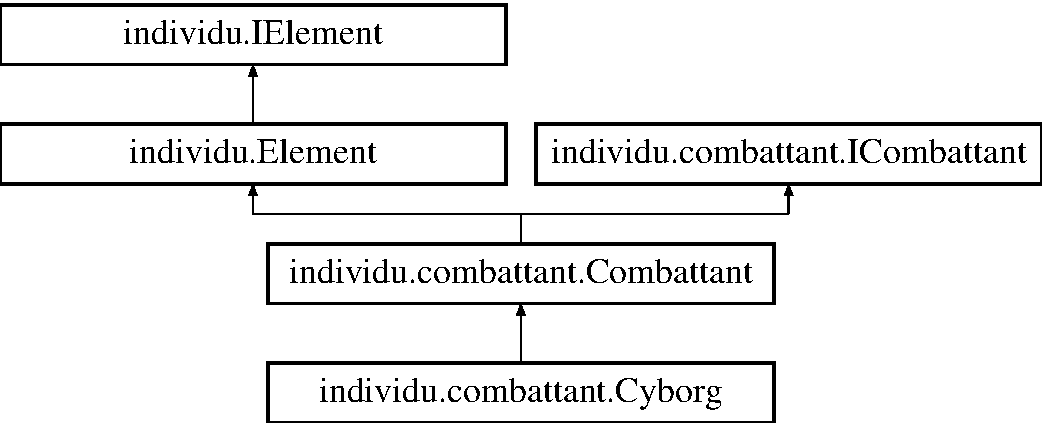
\includegraphics[height=4.000000cm]{classindividu_1_1combattant_1_1_cyborg}
\end{center}
\end{figure}
\subsection*{Fonctions membres publiques}
\begin{DoxyCompactItemize}
\item 
\hyperlink{classindividu_1_1combattant_1_1_cyborg_a62c5c65754e738dfa6db192c0e01a65e}{Cyborg} (String nom)
\end{DoxyCompactItemize}
\subsection*{Additional Inherited Members}


\subsection{Description détaillée}
Initialise un \hyperlink{classindividu_1_1combattant_1_1_combattant}{Combattant} avec les capacités d'un \hyperlink{classindividu_1_1combattant_1_1_cyborg}{Cyborg} 

\subsection{Documentation des constructeurs et destructeur}
\hypertarget{classindividu_1_1combattant_1_1_cyborg_a62c5c65754e738dfa6db192c0e01a65e}{\index{individu\-::combattant\-::\-Cyborg@{individu\-::combattant\-::\-Cyborg}!Cyborg@{Cyborg}}
\index{Cyborg@{Cyborg}!individu::combattant::Cyborg@{individu\-::combattant\-::\-Cyborg}}
\subsubsection[{Cyborg}]{\setlength{\rightskip}{0pt plus 5cm}individu.\-combattant.\-Cyborg.\-Cyborg (
\begin{DoxyParamCaption}
\item[{String}]{nom}
\end{DoxyParamCaption}
)}}\label{classindividu_1_1combattant_1_1_cyborg_a62c5c65754e738dfa6db192c0e01a65e}
Constructeur 
\begin{DoxyParams}{Paramètres}
{\em nom} & Le nom du \hyperlink{classindividu_1_1combattant_1_1_cyborg}{Cyborg} \\
\hline
\end{DoxyParams}


La documentation de cette classe a été générée à partir du fichier suivant \-:\begin{DoxyCompactItemize}
\item 
src/individu/combattant/Cyborg.\-java\end{DoxyCompactItemize}

\hypertarget{classinteraction_1_1_duel_basic}{\section{interaction.\-Duel\-Basic Class Reference}
\label{classinteraction_1_1_duel_basic}\index{interaction.\-Duel\-Basic@{interaction.\-Duel\-Basic}}
}
Inheritance diagram for interaction.\-Duel\-Basic\-:\begin{figure}[H]
\begin{center}
\leavevmode
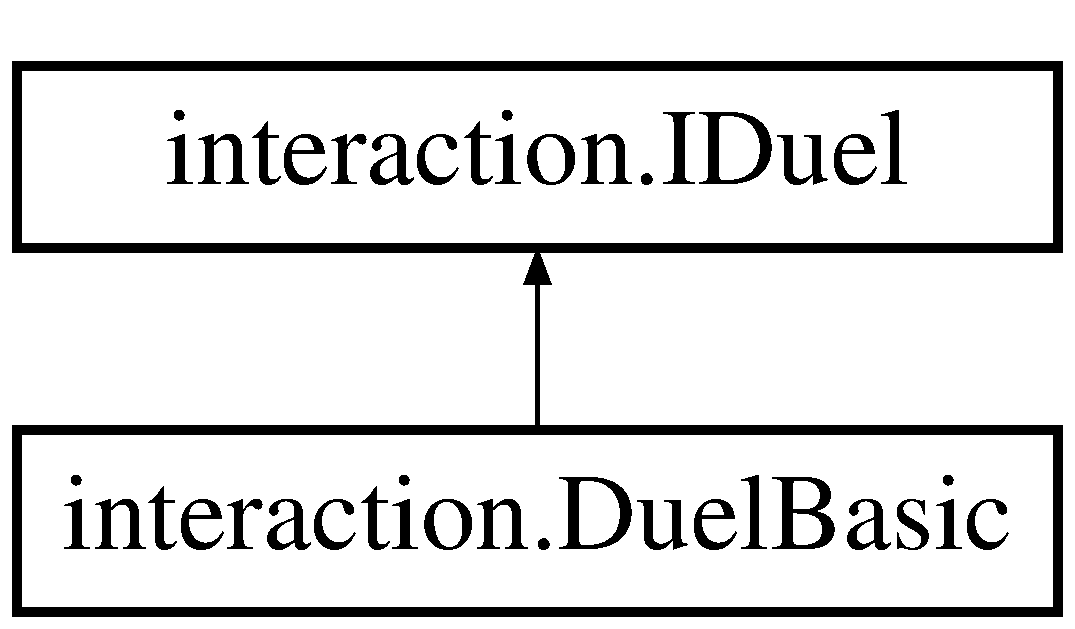
\includegraphics[height=2.000000cm]{classinteraction_1_1_duel_basic}
\end{center}
\end{figure}
\subsection*{Public Member Functions}
\begin{DoxyCompactItemize}
\item 
\hyperlink{classinteraction_1_1_duel_basic_afafe5b66524270a5acf3c855e896444e}{Duel\-Basic} (\hyperlink{classserveur_1_1_arene}{Arene} arene, Remote ref\-Attaquant, Remote ref\-Defenseur)  throws Remote\-Exception
\item 
int \hyperlink{classinteraction_1_1_duel_basic_a88b42733ab5e32f5334f1c590a6dcd72}{realiser\-Combat} ()  throws Remote\-Exception 
\item 
Remote \hyperlink{classinteraction_1_1_duel_basic_a406cd53e1eb8b51d99bbe8af72fb28d0}{get\-Ref\-Attaquant} ()  throws Remote\-Exception 
\item 
Remote \hyperlink{classinteraction_1_1_duel_basic_a6e7e4b0163230f13aad5ca285f969b6f}{get\-Ref\-Defenseur} ()  throws Remote\-Exception 
\end{DoxyCompactItemize}


\subsection{Constructor \& Destructor Documentation}
\hypertarget{classinteraction_1_1_duel_basic_afafe5b66524270a5acf3c855e896444e}{\index{interaction\-::\-Duel\-Basic@{interaction\-::\-Duel\-Basic}!Duel\-Basic@{Duel\-Basic}}
\index{Duel\-Basic@{Duel\-Basic}!interaction::DuelBasic@{interaction\-::\-Duel\-Basic}}
\subsubsection[{Duel\-Basic}]{\setlength{\rightskip}{0pt plus 5cm}interaction.\-Duel\-Basic.\-Duel\-Basic (
\begin{DoxyParamCaption}
\item[{{\bf Arene}}]{arene, }
\item[{Remote}]{ref\-Attaquant, }
\item[{Remote}]{ref\-Defenseur}
\end{DoxyParamCaption}
)  throws Remote\-Exception}}\label{classinteraction_1_1_duel_basic_afafe5b66524270a5acf3c855e896444e}
Constructeur 
\begin{DoxyParams}{Parameters}
{\em arene} & l'arene du jeu \\
\hline
{\em ref\-Attaquant} & la reference de l'attaquant \\
\hline
{\em ref\-Defenseur} & la reference du defenseur \\
\hline
\end{DoxyParams}

\begin{DoxyExceptions}{Exceptions}
{\em Remote\-Exception} & \\
\hline
\end{DoxyExceptions}


\subsection{Member Function Documentation}
\hypertarget{classinteraction_1_1_duel_basic_a406cd53e1eb8b51d99bbe8af72fb28d0}{\index{interaction\-::\-Duel\-Basic@{interaction\-::\-Duel\-Basic}!get\-Ref\-Attaquant@{get\-Ref\-Attaquant}}
\index{get\-Ref\-Attaquant@{get\-Ref\-Attaquant}!interaction::DuelBasic@{interaction\-::\-Duel\-Basic}}
\subsubsection[{get\-Ref\-Attaquant}]{\setlength{\rightskip}{0pt plus 5cm}Remote interaction.\-Duel\-Basic.\-get\-Ref\-Attaquant (
\begin{DoxyParamCaption}
{}
\end{DoxyParamCaption}
)  throws Remote\-Exception }}\label{classinteraction_1_1_duel_basic_a406cd53e1eb8b51d99bbe8af72fb28d0}
Renvoie la reference de l'attaquant connue par le serveur 
\begin{DoxyExceptions}{Exceptions}
{\em Remote\-Exception} & \\
\hline
\end{DoxyExceptions}


Implements \hyperlink{interfaceinteraction_1_1_i_duel_a17fc4fd253c7e9a02f3e0edf7680e67f}{interaction.\-I\-Duel}.

\hypertarget{classinteraction_1_1_duel_basic_a6e7e4b0163230f13aad5ca285f969b6f}{\index{interaction\-::\-Duel\-Basic@{interaction\-::\-Duel\-Basic}!get\-Ref\-Defenseur@{get\-Ref\-Defenseur}}
\index{get\-Ref\-Defenseur@{get\-Ref\-Defenseur}!interaction::DuelBasic@{interaction\-::\-Duel\-Basic}}
\subsubsection[{get\-Ref\-Defenseur}]{\setlength{\rightskip}{0pt plus 5cm}Remote interaction.\-Duel\-Basic.\-get\-Ref\-Defenseur (
\begin{DoxyParamCaption}
{}
\end{DoxyParamCaption}
)  throws Remote\-Exception }}\label{classinteraction_1_1_duel_basic_a6e7e4b0163230f13aad5ca285f969b6f}
Renvoie la reference du defenseur connue patr le serveur 
\begin{DoxyExceptions}{Exceptions}
{\em Remote\-Exception} & \\
\hline
\end{DoxyExceptions}


Implements \hyperlink{interfaceinteraction_1_1_i_duel_abc31afdeab5a1251c28bd6e61e828fe1}{interaction.\-I\-Duel}.

\hypertarget{classinteraction_1_1_duel_basic_a88b42733ab5e32f5334f1c590a6dcd72}{\index{interaction\-::\-Duel\-Basic@{interaction\-::\-Duel\-Basic}!realiser\-Combat@{realiser\-Combat}}
\index{realiser\-Combat@{realiser\-Combat}!interaction::DuelBasic@{interaction\-::\-Duel\-Basic}}
\subsubsection[{realiser\-Combat}]{\setlength{\rightskip}{0pt plus 5cm}int interaction.\-Duel\-Basic.\-realiser\-Combat (
\begin{DoxyParamCaption}
{}
\end{DoxyParamCaption}
)  throws Remote\-Exception }}\label{classinteraction_1_1_duel_basic_a88b42733ab5e32f5334f1c590a6dcd72}
Realise le combat 

Implements \hyperlink{interfaceinteraction_1_1_i_duel_a33a6e184f490717f27bed44b649814be}{interaction.\-I\-Duel}.



The documentation for this class was generated from the following file\-:\begin{DoxyCompactItemize}
\item 
src/interaction/Duel\-Basic.\-java\end{DoxyCompactItemize}

\hypertarget{classindividu_1_1_element}{\section{Référence de la classe individu.\-Element}
\label{classindividu_1_1_element}\index{individu.\-Element@{individu.\-Element}}
}
Graphe d'héritage de individu.\-Element\-:\begin{figure}[H]
\begin{center}
\leavevmode
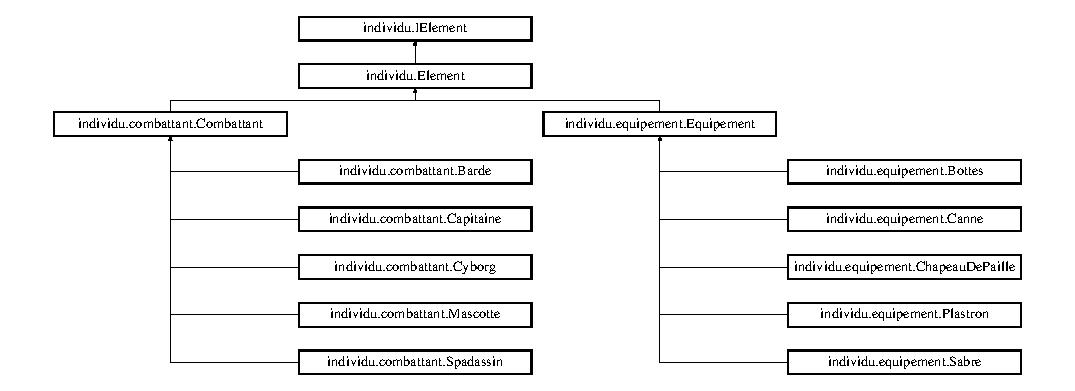
\includegraphics[height=4.806867cm]{classindividu_1_1_element}
\end{center}
\end{figure}
\subsection*{Fonctions membres publiques}
\begin{DoxyCompactItemize}
\item 
\hyperlink{classindividu_1_1_element_a5f9423f93dc30636b89b87580f328b69}{Element} (String nom)
\item 
\hyperlink{classindividu_1_1_element_a87447c2bac2e3725755526830863b6c9}{Element} (String p\-Nom, final int p\-Vie, final int p\-Vitesse, final int p\-Defense, final int p\-Attaque)
\item 
String \hyperlink{classindividu_1_1_element_a2623a37998d1558ad9d9f9352f833cd4}{get\-Nom} ()
\item 
int \hyperlink{classindividu_1_1_element_ab41f49b096712f65285de4437f1b15b5}{get\-Vie} ()
\item 
void \hyperlink{classindividu_1_1_element_ad8c8123352986a7e80dea748e34922cc}{set\-Vie} (int vie)
\item 
Array\-List$<$ Integer $>$ \hyperlink{classindividu_1_1_element_a46430a36f795bf42832317f96fdeeb5e}{get\-Elements\-Connus} ()
\item 
void \hyperlink{classindividu_1_1_element_aaaa713cc814adae8a8dda825263b48db}{ajouter\-Connu} (int ref)
\item 
String \hyperlink{classindividu_1_1_element_af4c2b08d92cfad7532168a5ccd6c2ebb}{to\-String} ()
\item 
int \hyperlink{classindividu_1_1_element_a4ccd4fbf75bf5f1020aba19b9c78d43d}{get\-Vitesse} ()
\item 
void \hyperlink{classindividu_1_1_element_a3b22be2d0831e60fc80748c6d50fce7b}{set\-Vitesse} (final int p\-Vitesse)
\item 
int \hyperlink{classindividu_1_1_element_a5dfa6bd163796694365cbd3f5aa1548d}{get\-Defense} ()
\item 
void \hyperlink{classindividu_1_1_element_a88a02d10762bebc68026a7d8e55fa368}{set\-Defense} (int p\-Defense)
\item 
int \hyperlink{classindividu_1_1_element_a911dfb782eeaf4d472189ee9f89e9c78}{get\-Attaque} ()
\item 
void \hyperlink{classindividu_1_1_element_a8b31860817a08081a17b8fdf79ecb15e}{set\-Attaque} (int p\-Attaque)
\item 
boolean \hyperlink{classindividu_1_1_element_a3f46bfb561b56c3e0eca8fe8de7c42be}{est\-Correct} ()
\end{DoxyCompactItemize}


\subsection{Description détaillée}
Classe générique pour les combattants et les Equipement implémentant \hyperlink{interfaceindividu_1_1_i_element}{I\-Element}. \begin{DoxySeeAlso}{Voir également}
Combattant 

Equipement 
\end{DoxySeeAlso}


\subsection{Documentation des constructeurs et destructeur}
\hypertarget{classindividu_1_1_element_a5f9423f93dc30636b89b87580f328b69}{\index{individu\-::\-Element@{individu\-::\-Element}!Element@{Element}}
\index{Element@{Element}!individu::Element@{individu\-::\-Element}}
\subsubsection[{Element}]{\setlength{\rightskip}{0pt plus 5cm}individu.\-Element.\-Element (
\begin{DoxyParamCaption}
\item[{String}]{nom}
\end{DoxyParamCaption}
)}}\label{classindividu_1_1_element_a5f9423f93dc30636b89b87580f328b69}
Constructeur initialisant toutes les valeurs à 0 
\begin{DoxyParams}{Paramètres}
{\em nom} & le nom de l'element a creer le nombre de vie est par defaut initialise a 1 \\
\hline
\end{DoxyParams}
\hypertarget{classindividu_1_1_element_a87447c2bac2e3725755526830863b6c9}{\index{individu\-::\-Element@{individu\-::\-Element}!Element@{Element}}
\index{Element@{Element}!individu::Element@{individu\-::\-Element}}
\subsubsection[{Element}]{\setlength{\rightskip}{0pt plus 5cm}individu.\-Element.\-Element (
\begin{DoxyParamCaption}
\item[{String}]{p\-Nom, }
\item[{final int}]{p\-Vie, }
\item[{final int}]{p\-Vitesse, }
\item[{final int}]{p\-Defense, }
\item[{final int}]{p\-Attaque}
\end{DoxyParamCaption}
)}}\label{classindividu_1_1_element_a87447c2bac2e3725755526830863b6c9}
\begin{DoxyVerb}Constructeur initialisant les valeurs à l'aide des paramètres
@param pNom Le nom le l'element a creer
\end{DoxyVerb}
 
\begin{DoxyParams}{Paramètres}
{\em p\-Vie} & Le nombre de vies initiales \\
\hline
{\em p\-Vitesse} & La vitesse permettant l'esquive \\
\hline
{\em p\-Defense} & La défense intiale \\
\hline
{\em p\-Attaque} & L'attaque initiale \\
\hline
\end{DoxyParams}


\subsection{Documentation des fonctions membres}
\hypertarget{classindividu_1_1_element_aaaa713cc814adae8a8dda825263b48db}{\index{individu\-::\-Element@{individu\-::\-Element}!ajouter\-Connu@{ajouter\-Connu}}
\index{ajouter\-Connu@{ajouter\-Connu}!individu::Element@{individu\-::\-Element}}
\subsubsection[{ajouter\-Connu}]{\setlength{\rightskip}{0pt plus 5cm}void individu.\-Element.\-ajouter\-Connu (
\begin{DoxyParamCaption}
\item[{int}]{ref}
\end{DoxyParamCaption}
)}}\label{classindividu_1_1_element_aaaa713cc814adae8a8dda825263b48db}

\begin{DoxyParams}{Paramètres}
{\em ref} & \\
\hline
\end{DoxyParams}


Implémente \hyperlink{interfaceindividu_1_1_i_element_a8c265785d6fb0f25cc54ec5850c602d3}{individu.\-I\-Element}.

\hypertarget{classindividu_1_1_element_a3f46bfb561b56c3e0eca8fe8de7c42be}{\index{individu\-::\-Element@{individu\-::\-Element}!est\-Correct@{est\-Correct}}
\index{est\-Correct@{est\-Correct}!individu::Element@{individu\-::\-Element}}
\subsubsection[{est\-Correct}]{\setlength{\rightskip}{0pt plus 5cm}boolean individu.\-Element.\-est\-Correct (
\begin{DoxyParamCaption}
{}
\end{DoxyParamCaption}
)}}\label{classindividu_1_1_element_a3f46bfb561b56c3e0eca8fe8de7c42be}
Retourne vrai si l'équation est respectée \begin{DoxyReturn}{Renvoie}
Vrai si équation respectée, faux sinon. 
\end{DoxyReturn}


Implémente \hyperlink{interfaceindividu_1_1_i_element_ab23f762049d3df68aa63a031023df646}{individu.\-I\-Element}.



Réimplémentée dans \hyperlink{classindividu_1_1equipement_1_1_equipement_a4c080bb12287c437a15e94e87a337688}{individu.\-equipement.\-Equipement}.

\hypertarget{classindividu_1_1_element_a911dfb782eeaf4d472189ee9f89e9c78}{\index{individu\-::\-Element@{individu\-::\-Element}!get\-Attaque@{get\-Attaque}}
\index{get\-Attaque@{get\-Attaque}!individu::Element@{individu\-::\-Element}}
\subsubsection[{get\-Attaque}]{\setlength{\rightskip}{0pt plus 5cm}int individu.\-Element.\-get\-Attaque (
\begin{DoxyParamCaption}
{}
\end{DoxyParamCaption}
)}}\label{classindividu_1_1_element_a911dfb782eeaf4d472189ee9f89e9c78}
\begin{DoxyReturn}{Renvoie}

\end{DoxyReturn}


Implémente \hyperlink{interfaceindividu_1_1_i_element_a2994427419f339274b17290846d259b9}{individu.\-I\-Element}.



Réimplémentée dans \hyperlink{classindividu_1_1combattant_1_1_combattant_ad63c7efc58a08fbd0e76f43e0bbccd68}{individu.\-combattant.\-Combattant}.

\hypertarget{classindividu_1_1_element_a5dfa6bd163796694365cbd3f5aa1548d}{\index{individu\-::\-Element@{individu\-::\-Element}!get\-Defense@{get\-Defense}}
\index{get\-Defense@{get\-Defense}!individu::Element@{individu\-::\-Element}}
\subsubsection[{get\-Defense}]{\setlength{\rightskip}{0pt plus 5cm}int individu.\-Element.\-get\-Defense (
\begin{DoxyParamCaption}
{}
\end{DoxyParamCaption}
)}}\label{classindividu_1_1_element_a5dfa6bd163796694365cbd3f5aa1548d}
\begin{DoxyReturn}{Renvoie}

\end{DoxyReturn}


Implémente \hyperlink{interfaceindividu_1_1_i_element_a9299fee825c29161f0e8bc401fbf36c3}{individu.\-I\-Element}.



Réimplémentée dans \hyperlink{classindividu_1_1combattant_1_1_combattant_afda5816b9a5d7c44d24e3a870c779754}{individu.\-combattant.\-Combattant}.

\hypertarget{classindividu_1_1_element_a46430a36f795bf42832317f96fdeeb5e}{\index{individu\-::\-Element@{individu\-::\-Element}!get\-Elements\-Connus@{get\-Elements\-Connus}}
\index{get\-Elements\-Connus@{get\-Elements\-Connus}!individu::Element@{individu\-::\-Element}}
\subsubsection[{get\-Elements\-Connus}]{\setlength{\rightskip}{0pt plus 5cm}Array\-List$<$Integer$>$ individu.\-Element.\-get\-Elements\-Connus (
\begin{DoxyParamCaption}
{}
\end{DoxyParamCaption}
)}}\label{classindividu_1_1_element_a46430a36f795bf42832317f96fdeeb5e}
\begin{DoxyReturn}{Renvoie}

\end{DoxyReturn}


Implémente \hyperlink{interfaceindividu_1_1_i_element_abb2ad9e31a3500c3c4deaaf58f9e01c9}{individu.\-I\-Element}.

\hypertarget{classindividu_1_1_element_a2623a37998d1558ad9d9f9352f833cd4}{\index{individu\-::\-Element@{individu\-::\-Element}!get\-Nom@{get\-Nom}}
\index{get\-Nom@{get\-Nom}!individu::Element@{individu\-::\-Element}}
\subsubsection[{get\-Nom}]{\setlength{\rightskip}{0pt plus 5cm}String individu.\-Element.\-get\-Nom (
\begin{DoxyParamCaption}
{}
\end{DoxyParamCaption}
)}}\label{classindividu_1_1_element_a2623a37998d1558ad9d9f9352f833cd4}
\begin{DoxyReturn}{Renvoie}

\end{DoxyReturn}


Implémente \hyperlink{interfaceindividu_1_1_i_element_a7783ed1b115d522ddd6a8a0c2aded632}{individu.\-I\-Element}.

\hypertarget{classindividu_1_1_element_ab41f49b096712f65285de4437f1b15b5}{\index{individu\-::\-Element@{individu\-::\-Element}!get\-Vie@{get\-Vie}}
\index{get\-Vie@{get\-Vie}!individu::Element@{individu\-::\-Element}}
\subsubsection[{get\-Vie}]{\setlength{\rightskip}{0pt plus 5cm}int individu.\-Element.\-get\-Vie (
\begin{DoxyParamCaption}
{}
\end{DoxyParamCaption}
)}}\label{classindividu_1_1_element_ab41f49b096712f65285de4437f1b15b5}
\begin{DoxyReturn}{Renvoie}

\end{DoxyReturn}


Implémente \hyperlink{interfaceindividu_1_1_i_element_a2f5272cb7b7f334bb9352cc2010c0abe}{individu.\-I\-Element}.

\hypertarget{classindividu_1_1_element_a4ccd4fbf75bf5f1020aba19b9c78d43d}{\index{individu\-::\-Element@{individu\-::\-Element}!get\-Vitesse@{get\-Vitesse}}
\index{get\-Vitesse@{get\-Vitesse}!individu::Element@{individu\-::\-Element}}
\subsubsection[{get\-Vitesse}]{\setlength{\rightskip}{0pt plus 5cm}int individu.\-Element.\-get\-Vitesse (
\begin{DoxyParamCaption}
{}
\end{DoxyParamCaption}
)}}\label{classindividu_1_1_element_a4ccd4fbf75bf5f1020aba19b9c78d43d}
\begin{DoxyReturn}{Renvoie}

\end{DoxyReturn}


Implémente \hyperlink{interfaceindividu_1_1_i_element_a824b3ce0b020526307476e9a50a98518}{individu.\-I\-Element}.



Réimplémentée dans \hyperlink{classindividu_1_1combattant_1_1_combattant_ad04833b8576cf9933e2c6dd3e04269e8}{individu.\-combattant.\-Combattant}.

\hypertarget{classindividu_1_1_element_a8b31860817a08081a17b8fdf79ecb15e}{\index{individu\-::\-Element@{individu\-::\-Element}!set\-Attaque@{set\-Attaque}}
\index{set\-Attaque@{set\-Attaque}!individu::Element@{individu\-::\-Element}}
\subsubsection[{set\-Attaque}]{\setlength{\rightskip}{0pt plus 5cm}void individu.\-Element.\-set\-Attaque (
\begin{DoxyParamCaption}
\item[{int}]{p\-Attaque}
\end{DoxyParamCaption}
)}}\label{classindividu_1_1_element_a8b31860817a08081a17b8fdf79ecb15e}

\begin{DoxyParams}{Paramètres}
{\em p\-Attaque} & \\
\hline
\end{DoxyParams}
\hypertarget{classindividu_1_1_element_a88a02d10762bebc68026a7d8e55fa368}{\index{individu\-::\-Element@{individu\-::\-Element}!set\-Defense@{set\-Defense}}
\index{set\-Defense@{set\-Defense}!individu::Element@{individu\-::\-Element}}
\subsubsection[{set\-Defense}]{\setlength{\rightskip}{0pt plus 5cm}void individu.\-Element.\-set\-Defense (
\begin{DoxyParamCaption}
\item[{int}]{p\-Defense}
\end{DoxyParamCaption}
)}}\label{classindividu_1_1_element_a88a02d10762bebc68026a7d8e55fa368}

\begin{DoxyParams}{Paramètres}
{\em p\-Defense} & \\
\hline
\end{DoxyParams}
\hypertarget{classindividu_1_1_element_ad8c8123352986a7e80dea748e34922cc}{\index{individu\-::\-Element@{individu\-::\-Element}!set\-Vie@{set\-Vie}}
\index{set\-Vie@{set\-Vie}!individu::Element@{individu\-::\-Element}}
\subsubsection[{set\-Vie}]{\setlength{\rightskip}{0pt plus 5cm}void individu.\-Element.\-set\-Vie (
\begin{DoxyParamCaption}
\item[{int}]{vie}
\end{DoxyParamCaption}
)}}\label{classindividu_1_1_element_ad8c8123352986a7e80dea748e34922cc}

\begin{DoxyParams}{Paramètres}
{\em vie} & \\
\hline
\end{DoxyParams}


Implémente \hyperlink{interfaceindividu_1_1_i_element_a386d0b896afaf5481da8c6f667b11297}{individu.\-I\-Element}.

\hypertarget{classindividu_1_1_element_a3b22be2d0831e60fc80748c6d50fce7b}{\index{individu\-::\-Element@{individu\-::\-Element}!set\-Vitesse@{set\-Vitesse}}
\index{set\-Vitesse@{set\-Vitesse}!individu::Element@{individu\-::\-Element}}
\subsubsection[{set\-Vitesse}]{\setlength{\rightskip}{0pt plus 5cm}void individu.\-Element.\-set\-Vitesse (
\begin{DoxyParamCaption}
\item[{final int}]{p\-Vitesse}
\end{DoxyParamCaption}
)}}\label{classindividu_1_1_element_a3b22be2d0831e60fc80748c6d50fce7b}

\begin{DoxyParams}{Paramètres}
{\em p\-Vitesse} & \\
\hline
\end{DoxyParams}


Implémente \hyperlink{interfaceindividu_1_1_i_element_a50c000c10b016186ff3becd67ae5d5ae}{individu.\-I\-Element}.

\hypertarget{classindividu_1_1_element_af4c2b08d92cfad7532168a5ccd6c2ebb}{\index{individu\-::\-Element@{individu\-::\-Element}!to\-String@{to\-String}}
\index{to\-String@{to\-String}!individu::Element@{individu\-::\-Element}}
\subsubsection[{to\-String}]{\setlength{\rightskip}{0pt plus 5cm}String individu.\-Element.\-to\-String (
\begin{DoxyParamCaption}
{}
\end{DoxyParamCaption}
)}}\label{classindividu_1_1_element_af4c2b08d92cfad7532168a5ccd6c2ebb}
\begin{DoxyReturn}{Renvoie}

\end{DoxyReturn}


Implémente \hyperlink{interfaceindividu_1_1_i_element_a4609baa01e8f8558e931b2f8901e789d}{individu.\-I\-Element}.



La documentation de cette classe a été générée à partir du fichier suivant \-:\begin{DoxyCompactItemize}
\item 
src/individu/Element.\-java\end{DoxyCompactItemize}

\hypertarget{classindividu_1_1equipement_1_1_equipement}{\section{Référence de la classe individu.\-equipement.\-Equipement}
\label{classindividu_1_1equipement_1_1_equipement}\index{individu.\-equipement.\-Equipement@{individu.\-equipement.\-Equipement}}
}
Graphe d'héritage de individu.\-equipement.\-Equipement\-:\begin{figure}[H]
\begin{center}
\leavevmode
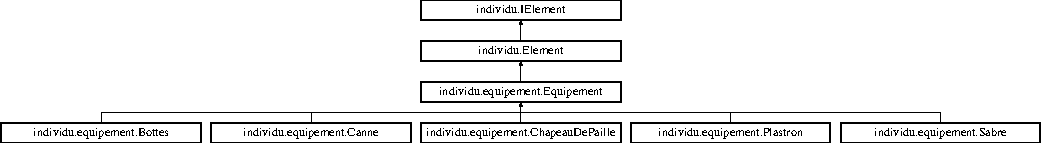
\includegraphics[height=1.922747cm]{classindividu_1_1equipement_1_1_equipement}
\end{center}
\end{figure}
\subsection*{Fonctions membres publiques}
\begin{DoxyCompactItemize}
\item 
\hypertarget{classindividu_1_1equipement_1_1_equipement_ab3495255f9c6ae3e41e93c1aae3cf45d}{{\bfseries Equipement} (String nom)}\label{classindividu_1_1equipement_1_1_equipement_ab3495255f9c6ae3e41e93c1aae3cf45d}

\item 
\hypertarget{classindividu_1_1equipement_1_1_equipement_a801846813aa092406eaeb40ec265820e}{int {\bfseries get\-Duree} ()}\label{classindividu_1_1equipement_1_1_equipement_a801846813aa092406eaeb40ec265820e}

\item 
\hypertarget{classindividu_1_1equipement_1_1_equipement_a666480fb37b0e76e607868ebf3b8d6c2}{void {\bfseries set\-Duree} (int p\-Duree)}\label{classindividu_1_1equipement_1_1_equipement_a666480fb37b0e76e607868ebf3b8d6c2}

\end{DoxyCompactItemize}


La documentation de cette classe a été générée à partir du fichier suivant \-:\begin{DoxyCompactItemize}
\item 
src/individu/equipement/Equipement.\-java\end{DoxyCompactItemize}

\hypertarget{interfaceserveur_1_1_i_arene}{\section{Référence de l'interface serveur.\-I\-Arene}
\label{interfaceserveur_1_1_i_arene}\index{serveur.\-I\-Arene@{serveur.\-I\-Arene}}
}
Graphe d'héritage de serveur.\-I\-Arene\-:\begin{figure}[H]
\begin{center}
\leavevmode
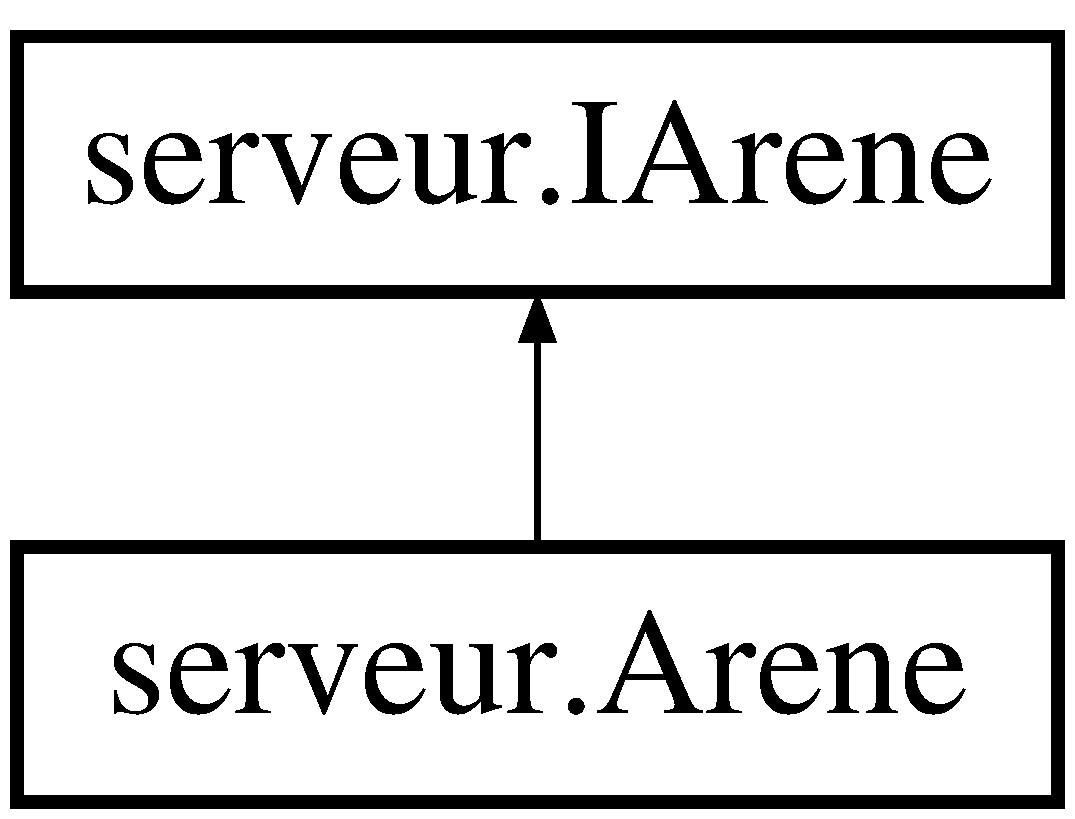
\includegraphics[height=2.000000cm]{interfaceserveur_1_1_i_arene}
\end{center}
\end{figure}
\subsection*{Fonctions membres publiques}
\begin{DoxyCompactItemize}
\item 
int \hyperlink{interfaceserveur_1_1_i_arene_a6dc6a07ca0fdb5c2fd1ba53edd132298}{allocate\-Ref} ()  throws Remote\-Exception
\item 
void \hyperlink{interfaceserveur_1_1_i_arene_a5a051d16e51b7a0f368c4f89401a0293}{connect} (\hyperlink{classinterface_graphique_1_1_vue_element}{Vue\-Element} ve)  throws Remote\-Exception
\item 
Array\-List$<$ \hyperlink{classinterface_graphique_1_1_vue_element}{Vue\-Element} $>$ \hyperlink{interfaceserveur_1_1_i_arene_ab7ea50f885f2cf28628d1c7ce2ca0159}{get\-World} ()  throws Remote\-Exception
\item 
Hashtable$<$ Integer, \hyperlink{classinterface_graphique_1_1_vue_element}{Vue\-Element} $>$ \hyperlink{interfaceserveur_1_1_i_arene_a47a37dbadfd6418b184e2c9f41faec01}{voisins} (Point pos, int ref)  throws Remote\-Exception
\item 
void \hyperlink{interfaceserveur_1_1_i_arene_aec66c3ded2467e80685b8cb4cf856cbc}{interaction} (int ref, int ref2)  throws Remote\-Exception
\item 
void \hyperlink{interfaceserveur_1_1_i_arene_adc0a9a0ec4b423e5b6a13a90091ead8c}{ramasser} (int ref, int ref2)  throws Remote\-Exception
\end{DoxyCompactItemize}


\subsection{Description détaillée}
Interface de l'\hyperlink{classserveur_1_1_arene}{Arene} 

\subsection{Documentation des fonctions membres}
\hypertarget{interfaceserveur_1_1_i_arene_a6dc6a07ca0fdb5c2fd1ba53edd132298}{\index{serveur\-::\-I\-Arene@{serveur\-::\-I\-Arene}!allocate\-Ref@{allocate\-Ref}}
\index{allocate\-Ref@{allocate\-Ref}!serveur::IArene@{serveur\-::\-I\-Arene}}
\subsubsection[{allocate\-Ref}]{\setlength{\rightskip}{0pt plus 5cm}int serveur.\-I\-Arene.\-allocate\-Ref (
\begin{DoxyParamCaption}
{}
\end{DoxyParamCaption}
)  throws Remote\-Exception}}\label{interfaceserveur_1_1_i_arene_a6dc6a07ca0fdb5c2fd1ba53edd132298}
Renvoie une reference pour la console en train de se connecter 
\begin{DoxyExceptions}{Exceptions}
{\em Remote\-Exception} & \\
\hline
\end{DoxyExceptions}


Implémenté dans \hyperlink{classserveur_1_1_arene_a88151079f2665d1973168e0cb266e3c7}{serveur.\-Arene}.

\hypertarget{interfaceserveur_1_1_i_arene_a5a051d16e51b7a0f368c4f89401a0293}{\index{serveur\-::\-I\-Arene@{serveur\-::\-I\-Arene}!connect@{connect}}
\index{connect@{connect}!serveur::IArene@{serveur\-::\-I\-Arene}}
\subsubsection[{connect}]{\setlength{\rightskip}{0pt plus 5cm}void serveur.\-I\-Arene.\-connect (
\begin{DoxyParamCaption}
\item[{{\bf Vue\-Element}}]{ve}
\end{DoxyParamCaption}
)  throws Remote\-Exception}}\label{interfaceserveur_1_1_i_arene_a5a051d16e51b7a0f368c4f89401a0293}
Connexion d'un element au serveur 
\begin{DoxyParams}{Paramètres}
{\em ve} & la vue de l'element a se connecter \\
\hline
\end{DoxyParams}

\begin{DoxyExceptions}{Exceptions}
{\em Remote\-Exception} & \\
\hline
\end{DoxyExceptions}


Implémenté dans \hyperlink{classserveur_1_1_arene_aa0f409b1844a97c1c413f04116cf863e}{serveur.\-Arene}.

\hypertarget{interfaceserveur_1_1_i_arene_ab7ea50f885f2cf28628d1c7ce2ca0159}{\index{serveur\-::\-I\-Arene@{serveur\-::\-I\-Arene}!get\-World@{get\-World}}
\index{get\-World@{get\-World}!serveur::IArene@{serveur\-::\-I\-Arene}}
\subsubsection[{get\-World}]{\setlength{\rightskip}{0pt plus 5cm}Array\-List$<${\bf Vue\-Element}$>$ serveur.\-I\-Arene.\-get\-World (
\begin{DoxyParamCaption}
{}
\end{DoxyParamCaption}
)  throws Remote\-Exception}}\label{interfaceserveur_1_1_i_arene_ab7ea50f885f2cf28628d1c7ce2ca0159}
Calcule la liste de toutes les representations d'elements presentes dans l'arene. \begin{DoxyReturn}{Renvoie}
la liste des representations 
\end{DoxyReturn}

\begin{DoxyExceptions}{Exceptions}
{\em Remote\-Exception} & \\
\hline
\end{DoxyExceptions}


Implémenté dans \hyperlink{classserveur_1_1_arene_a83fb30e5a71d573d180997e60ab41304}{serveur.\-Arene}.

\hypertarget{interfaceserveur_1_1_i_arene_aec66c3ded2467e80685b8cb4cf856cbc}{\index{serveur\-::\-I\-Arene@{serveur\-::\-I\-Arene}!interaction@{interaction}}
\index{interaction@{interaction}!serveur::IArene@{serveur\-::\-I\-Arene}}
\subsubsection[{interaction}]{\setlength{\rightskip}{0pt plus 5cm}void serveur.\-I\-Arene.\-interaction (
\begin{DoxyParamCaption}
\item[{int}]{ref, }
\item[{int}]{ref2}
\end{DoxyParamCaption}
)  throws Remote\-Exception}}\label{interfaceserveur_1_1_i_arene_aec66c3ded2467e80685b8cb4cf856cbc}
Methode d'interaction (combat) entre deux elements dont on a la reference 
\begin{DoxyParams}{Paramètres}
{\em ref} & le premier element \\
\hline
{\em ref2} & le deuxieme element \\
\hline
\end{DoxyParams}

\begin{DoxyExceptions}{Exceptions}
{\em Remote\-Exception} & \\
\hline
\end{DoxyExceptions}


Implémenté dans \hyperlink{classserveur_1_1_arene_ae8331f4b3d827f4c93d4b1c08a0d9399}{serveur.\-Arene}.

\hypertarget{interfaceserveur_1_1_i_arene_adc0a9a0ec4b423e5b6a13a90091ead8c}{\index{serveur\-::\-I\-Arene@{serveur\-::\-I\-Arene}!ramasser@{ramasser}}
\index{ramasser@{ramasser}!serveur::IArene@{serveur\-::\-I\-Arene}}
\subsubsection[{ramasser}]{\setlength{\rightskip}{0pt plus 5cm}void serveur.\-I\-Arene.\-ramasser (
\begin{DoxyParamCaption}
\item[{int}]{ref, }
\item[{int}]{ref2}
\end{DoxyParamCaption}
)  throws Remote\-Exception}}\label{interfaceserveur_1_1_i_arene_adc0a9a0ec4b423e5b6a13a90091ead8c}
Ramassage de l'equipement par le comabattant 
\begin{DoxyParams}{Paramètres}
{\em ref} & le combattant \\
\hline
{\em ref2} & l'objet a ramasser \\
\hline
\end{DoxyParams}

\begin{DoxyExceptions}{Exceptions}
{\em Remote\-Exception} & \\
\hline
\end{DoxyExceptions}


Implémenté dans \hyperlink{classserveur_1_1_arene_a930bd7387f12b44bcbfdc117fbd13672}{serveur.\-Arene}.

\hypertarget{interfaceserveur_1_1_i_arene_a47a37dbadfd6418b184e2c9f41faec01}{\index{serveur\-::\-I\-Arene@{serveur\-::\-I\-Arene}!voisins@{voisins}}
\index{voisins@{voisins}!serveur::IArene@{serveur\-::\-I\-Arene}}
\subsubsection[{voisins}]{\setlength{\rightskip}{0pt plus 5cm}Hashtable$<$Integer, {\bf Vue\-Element}$>$ serveur.\-I\-Arene.\-voisins (
\begin{DoxyParamCaption}
\item[{Point}]{pos, }
\item[{int}]{ref}
\end{DoxyParamCaption}
)  throws Remote\-Exception}}\label{interfaceserveur_1_1_i_arene_a47a37dbadfd6418b184e2c9f41faec01}
Liste les voisins (representations d'element) d'une coordonnee dans l'arene sous la forme de couples (reference,coordonnees) dans une Hashtable 
\begin{DoxyExceptions}{Exceptions}
{\em Remote\-Exception} & \\
\hline
\end{DoxyExceptions}


Implémenté dans \hyperlink{classserveur_1_1_arene_a1b8ef284b2fae162ba68884bfbe0160a}{serveur.\-Arene}.



La documentation de cette interface a été générée à partir du fichier suivant \-:\begin{DoxyCompactItemize}
\item 
src/serveur/I\-Arene.\-java\end{DoxyCompactItemize}

\hypertarget{interfaceindividu_1_1combattant_1_1_i_combattant}{\section{Référence de l'interface individu.\-combattant.\-I\-Combattant}
\label{interfaceindividu_1_1combattant_1_1_i_combattant}\index{individu.\-combattant.\-I\-Combattant@{individu.\-combattant.\-I\-Combattant}}
}
Graphe d'héritage de individu.\-combattant.\-I\-Combattant\-:\begin{figure}[H]
\begin{center}
\leavevmode
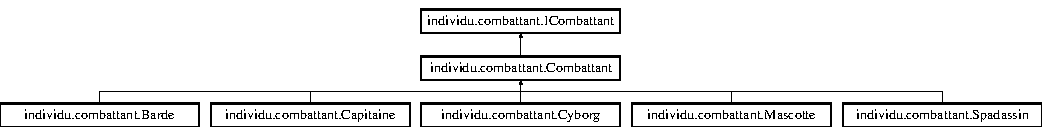
\includegraphics[height=1.705584cm]{interfaceindividu_1_1combattant_1_1_i_combattant}
\end{center}
\end{figure}
\subsection*{Fonctions membres publiques}
\begin{DoxyCompactItemize}
\item 
void \hyperlink{interfaceindividu_1_1combattant_1_1_i_combattant_a8b656cde577f3346cee0f75450cbcb42}{gagner} (int s)
\item 
void \hyperlink{interfaceindividu_1_1combattant_1_1_i_combattant_a762a6a778b7a09fa32564e6dd9e0aa46}{perdre} (int s)
\item 
void \hyperlink{interfaceindividu_1_1combattant_1_1_i_combattant_a48e6090fc4b67a81a8028477ea6b15e7}{ramasser} (int ref)
\item 
void \hyperlink{interfaceindividu_1_1combattant_1_1_i_combattant_aca0de8e3df27d07ceb216e022c403cc6}{set\-Nb\-Objets} (final int p\-Nb\-Objets)
\item 
int \hyperlink{interfaceindividu_1_1combattant_1_1_i_combattant_abf39b472bad06221d901d2d143ee5c91}{get\-Nb\-Objets} ()
\item 
void \hyperlink{interfaceindividu_1_1combattant_1_1_i_combattant_abaa834896ead5ad778a23edaccf61148}{set\-Argent} (final int p\-Argent)
\item 
int \hyperlink{interfaceindividu_1_1combattant_1_1_i_combattant_a820ac1fbe763b07ae4300a58f6fc0463}{get\-Argent} ()
\end{DoxyCompactItemize}


\subsection{Documentation des fonctions membres}
\hypertarget{interfaceindividu_1_1combattant_1_1_i_combattant_a8b656cde577f3346cee0f75450cbcb42}{\index{individu\-::combattant\-::\-I\-Combattant@{individu\-::combattant\-::\-I\-Combattant}!gagner@{gagner}}
\index{gagner@{gagner}!individu::combattant::ICombattant@{individu\-::combattant\-::\-I\-Combattant}}
\subsubsection[{gagner}]{\setlength{\rightskip}{0pt plus 5cm}void individu.\-combattant.\-I\-Combattant.\-gagner (
\begin{DoxyParamCaption}
\item[{int}]{s}
\end{DoxyParamCaption}
)}}\label{interfaceindividu_1_1combattant_1_1_i_combattant_a8b656cde577f3346cee0f75450cbcb42}
Mets a jour l'argent que le combattant a gagne 
\begin{DoxyParams}{Paramètres}
{\em s} & le montant gagne \\
\hline
\end{DoxyParams}


Implémenté dans \hyperlink{classindividu_1_1combattant_1_1_combattant_a2cf4b27020ffa07f6b6770dfd1654bc4}{individu.\-combattant.\-Combattant}.

\hypertarget{interfaceindividu_1_1combattant_1_1_i_combattant_a820ac1fbe763b07ae4300a58f6fc0463}{\index{individu\-::combattant\-::\-I\-Combattant@{individu\-::combattant\-::\-I\-Combattant}!get\-Argent@{get\-Argent}}
\index{get\-Argent@{get\-Argent}!individu::combattant::ICombattant@{individu\-::combattant\-::\-I\-Combattant}}
\subsubsection[{get\-Argent}]{\setlength{\rightskip}{0pt plus 5cm}int individu.\-combattant.\-I\-Combattant.\-get\-Argent (
\begin{DoxyParamCaption}
{}
\end{DoxyParamCaption}
)}}\label{interfaceindividu_1_1combattant_1_1_i_combattant_a820ac1fbe763b07ae4300a58f6fc0463}
Retourne la quantité d'argent du combattant \begin{DoxyReturn}{Renvoie}
La quantité d'argent 
\end{DoxyReturn}


Implémenté dans \hyperlink{classindividu_1_1combattant_1_1_combattant_a1a6e4767d3b9bae8e913c427db5ffc64}{individu.\-combattant.\-Combattant}.

\hypertarget{interfaceindividu_1_1combattant_1_1_i_combattant_abf39b472bad06221d901d2d143ee5c91}{\index{individu\-::combattant\-::\-I\-Combattant@{individu\-::combattant\-::\-I\-Combattant}!get\-Nb\-Objets@{get\-Nb\-Objets}}
\index{get\-Nb\-Objets@{get\-Nb\-Objets}!individu::combattant::ICombattant@{individu\-::combattant\-::\-I\-Combattant}}
\subsubsection[{get\-Nb\-Objets}]{\setlength{\rightskip}{0pt plus 5cm}int individu.\-combattant.\-I\-Combattant.\-get\-Nb\-Objets (
\begin{DoxyParamCaption}
{}
\end{DoxyParamCaption}
)}}\label{interfaceindividu_1_1combattant_1_1_i_combattant_abf39b472bad06221d901d2d143ee5c91}
Retourne le nombre d'objets maximum que peut porter un combattant \begin{DoxyReturn}{Renvoie}
Le nombre d'objet 
\end{DoxyReturn}


Implémenté dans \hyperlink{classindividu_1_1combattant_1_1_combattant_afe9afbb1b4d2b169054d1b3b31c1c362}{individu.\-combattant.\-Combattant}.

\hypertarget{interfaceindividu_1_1combattant_1_1_i_combattant_a762a6a778b7a09fa32564e6dd9e0aa46}{\index{individu\-::combattant\-::\-I\-Combattant@{individu\-::combattant\-::\-I\-Combattant}!perdre@{perdre}}
\index{perdre@{perdre}!individu::combattant::ICombattant@{individu\-::combattant\-::\-I\-Combattant}}
\subsubsection[{perdre}]{\setlength{\rightskip}{0pt plus 5cm}void individu.\-combattant.\-I\-Combattant.\-perdre (
\begin{DoxyParamCaption}
\item[{int}]{s}
\end{DoxyParamCaption}
)}}\label{interfaceindividu_1_1combattant_1_1_i_combattant_a762a6a778b7a09fa32564e6dd9e0aa46}
Mets a jour l'argent que le combattant a perdu 
\begin{DoxyParams}{Paramètres}
{\em s} & l'argent perdu \\
\hline
\end{DoxyParams}


Implémenté dans \hyperlink{classindividu_1_1combattant_1_1_combattant_a46767973062954ee738e28856f1b6c6e}{individu.\-combattant.\-Combattant}.

\hypertarget{interfaceindividu_1_1combattant_1_1_i_combattant_a48e6090fc4b67a81a8028477ea6b15e7}{\index{individu\-::combattant\-::\-I\-Combattant@{individu\-::combattant\-::\-I\-Combattant}!ramasser@{ramasser}}
\index{ramasser@{ramasser}!individu::combattant::ICombattant@{individu\-::combattant\-::\-I\-Combattant}}
\subsubsection[{ramasser}]{\setlength{\rightskip}{0pt plus 5cm}void individu.\-combattant.\-I\-Combattant.\-ramasser (
\begin{DoxyParamCaption}
\item[{int}]{ref}
\end{DoxyParamCaption}
)}}\label{interfaceindividu_1_1combattant_1_1_i_combattant_a48e6090fc4b67a81a8028477ea6b15e7}
Mets a jour la liste des objets ramasses par le combattant 
\begin{DoxyParams}{Paramètres}
{\em ref} & la reference (serveur) d'un equipement a ramasser \\
\hline
\end{DoxyParams}


Implémenté dans \hyperlink{classindividu_1_1combattant_1_1_combattant_a7d56bc66f5eab04efdeeb748e29d1859}{individu.\-combattant.\-Combattant}.

\hypertarget{interfaceindividu_1_1combattant_1_1_i_combattant_abaa834896ead5ad778a23edaccf61148}{\index{individu\-::combattant\-::\-I\-Combattant@{individu\-::combattant\-::\-I\-Combattant}!set\-Argent@{set\-Argent}}
\index{set\-Argent@{set\-Argent}!individu::combattant::ICombattant@{individu\-::combattant\-::\-I\-Combattant}}
\subsubsection[{set\-Argent}]{\setlength{\rightskip}{0pt plus 5cm}void individu.\-combattant.\-I\-Combattant.\-set\-Argent (
\begin{DoxyParamCaption}
\item[{final int}]{p\-Argent}
\end{DoxyParamCaption}
)}}\label{interfaceindividu_1_1combattant_1_1_i_combattant_abaa834896ead5ad778a23edaccf61148}
Réinitialie la quantité d'argent d'un combattant 
\begin{DoxyParams}{Paramètres}
{\em p\-Argent} & La nouvelle quantité d'argent \\
\hline
\end{DoxyParams}
\hypertarget{interfaceindividu_1_1combattant_1_1_i_combattant_aca0de8e3df27d07ceb216e022c403cc6}{\index{individu\-::combattant\-::\-I\-Combattant@{individu\-::combattant\-::\-I\-Combattant}!set\-Nb\-Objets@{set\-Nb\-Objets}}
\index{set\-Nb\-Objets@{set\-Nb\-Objets}!individu::combattant::ICombattant@{individu\-::combattant\-::\-I\-Combattant}}
\subsubsection[{set\-Nb\-Objets}]{\setlength{\rightskip}{0pt plus 5cm}void individu.\-combattant.\-I\-Combattant.\-set\-Nb\-Objets (
\begin{DoxyParamCaption}
\item[{final int}]{p\-Nb\-Objets}
\end{DoxyParamCaption}
)}}\label{interfaceindividu_1_1combattant_1_1_i_combattant_aca0de8e3df27d07ceb216e022c403cc6}
Réinitialise le nombre d'objets maximum que peut porter un combattant 
\begin{DoxyParams}{Paramètres}
{\em p\-Nb\-Objets} & Le nouveau nombre d'objet \\
\hline
\end{DoxyParams}


Implémenté dans \hyperlink{classindividu_1_1combattant_1_1_combattant_a127950f43fa0397daa5e23616bf6340c}{individu.\-combattant.\-Combattant}.



La documentation de cette interface a été générée à partir du fichier suivant \-:\begin{DoxyCompactItemize}
\item 
src/individu/combattant/I\-Combattant.\-java\end{DoxyCompactItemize}

\hypertarget{interfacecontrole_1_1_i_console}{\section{Référence de l'interface controle.\-I\-Console}
\label{interfacecontrole_1_1_i_console}\index{controle.\-I\-Console@{controle.\-I\-Console}}
}
Graphe d'héritage de controle.\-I\-Console\-:\begin{figure}[H]
\begin{center}
\leavevmode
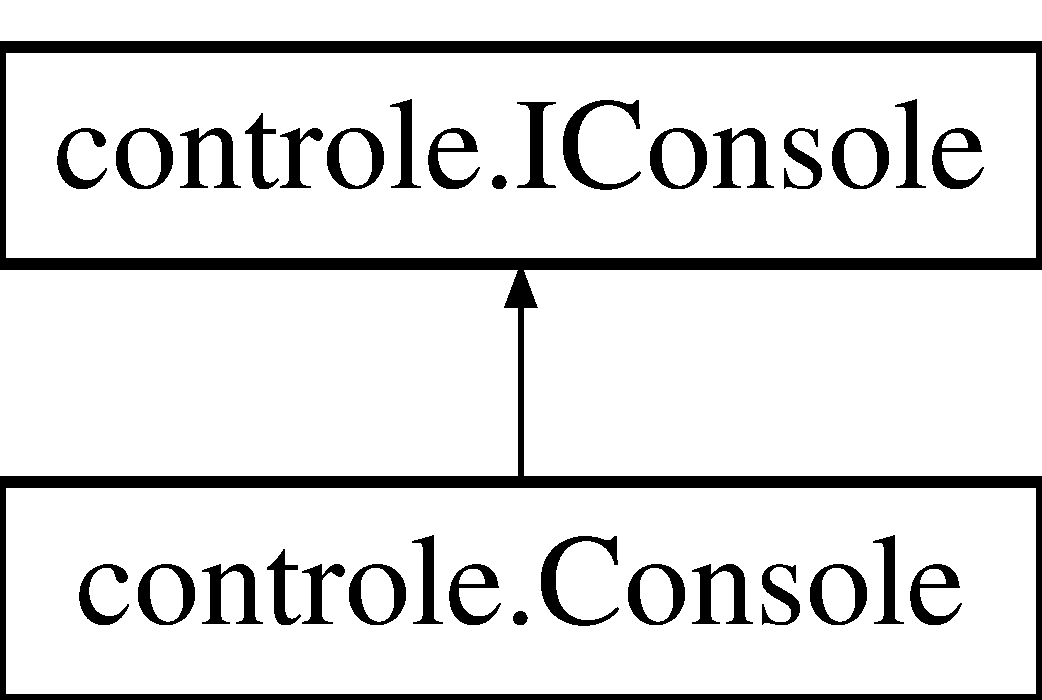
\includegraphics[height=2.000000cm]{interfacecontrole_1_1_i_console}
\end{center}
\end{figure}
\subsection*{Fonctions membres publiques}
\begin{DoxyCompactItemize}
\item 
void \hyperlink{interfacecontrole_1_1_i_console_a77e327568514ec7eed8161c6b73e4d9a}{shut\-Down} (String cause)  throws Remote\-Exception
\item 
void \hyperlink{interfacecontrole_1_1_i_console_afb2a3e548fe438ac7af6bc429fc84132}{run} ()  throws Remote\-Exception
\item 
\hyperlink{classinterface_graphique_1_1_vue_element}{Vue\-Element} \hyperlink{interfacecontrole_1_1_i_console_ab6728a4bf807f04e5d13bfd452a69bc2}{update} ()  throws Remote\-Exception
\item 
void \hyperlink{interfacecontrole_1_1_i_console_ac0aefd004a73641f8ba6ef57266c0508}{ajouter\-Connu} (int ref)  throws Remote\-Exception
\item 
\hyperlink{classindividu_1_1_element}{Element} \hyperlink{interfacecontrole_1_1_i_console_a0cde95415052505230b482a2b5fed5fd}{get\-Element} ()  throws Remote\-Exception
\item 
\hyperlink{classinterface_graphique_1_1_vue_element}{Vue\-Element} \hyperlink{interfacecontrole_1_1_i_console_a5fc11711131f9a99768d36bffc695535}{get\-Vue\-Element} ()  throws Remote\-Exception
\item 
void \hyperlink{interfacecontrole_1_1_i_console_ab200b6a49e88391691be5df49cfa36f2}{parler} (String message)  throws Remote\-Exception
\item 
void \hyperlink{interfacecontrole_1_1_i_console_ace6ee762b3f067e26f478066a9c1283f}{perdre\-Vie} (int vie\-Perdue)  throws Remote\-Exception
\item 
void \hyperlink{interfacecontrole_1_1_i_console_a90d8826ee94075bc55a52779a0257b85}{ramasser\-Objet} (\hyperlink{interfacecontrole_1_1_i_console}{I\-Console} objet)  throws Remote\-Exception
\item 
String \hyperlink{interfacecontrole_1_1_i_console_a6166aa60251707f3c095e8e197a88dac}{afficher} ()  throws Remote\-Exception
\end{DoxyCompactItemize}


\subsection{Description détaillée}
Represente le lien Element -\/ Serveur 

\subsection{Documentation des fonctions membres}
\hypertarget{interfacecontrole_1_1_i_console_a6166aa60251707f3c095e8e197a88dac}{\index{controle\-::\-I\-Console@{controle\-::\-I\-Console}!afficher@{afficher}}
\index{afficher@{afficher}!controle::IConsole@{controle\-::\-I\-Console}}
\subsubsection[{afficher}]{\setlength{\rightskip}{0pt plus 5cm}String controle.\-I\-Console.\-afficher (
\begin{DoxyParamCaption}
{}
\end{DoxyParamCaption}
)  throws Remote\-Exception}}\label{interfacecontrole_1_1_i_console_a6166aa60251707f3c095e8e197a88dac}
\begin{DoxyVerb}Renvoie l'etat de l'element a afficher sur l'interface graphique
\end{DoxyVerb}
 \begin{DoxyReturn}{Renvoie}

\end{DoxyReturn}

\begin{DoxyExceptions}{Exceptions}
{\em Remote\-Exception} & \\
\hline
\end{DoxyExceptions}


Implémenté dans \hyperlink{classcontrole_1_1_console_a750f2122aee6e608375f999cdfa5f43b}{controle.\-Console}.

\hypertarget{interfacecontrole_1_1_i_console_ac0aefd004a73641f8ba6ef57266c0508}{\index{controle\-::\-I\-Console@{controle\-::\-I\-Console}!ajouter\-Connu@{ajouter\-Connu}}
\index{ajouter\-Connu@{ajouter\-Connu}!controle::IConsole@{controle\-::\-I\-Console}}
\subsubsection[{ajouter\-Connu}]{\setlength{\rightskip}{0pt plus 5cm}void controle.\-I\-Console.\-ajouter\-Connu (
\begin{DoxyParamCaption}
\item[{int}]{ref}
\end{DoxyParamCaption}
)  throws Remote\-Exception}}\label{interfacecontrole_1_1_i_console_ac0aefd004a73641f8ba6ef57266c0508}
Ajout a l'element celui avec lequel il a joue/ qu'il a ramasse 
\begin{DoxyParams}{Paramètres}
{\em ref} & l'element avec lequel l'objet courrant a joue/ramasse \\
\hline
\end{DoxyParams}

\begin{DoxyExceptions}{Exceptions}
{\em Remote\-Exception} & \\
\hline
\end{DoxyExceptions}


Implémenté dans \hyperlink{classcontrole_1_1_console_aae7e697a8bc845c11c1430c08edd6b8c}{controle.\-Console}.

\hypertarget{interfacecontrole_1_1_i_console_a0cde95415052505230b482a2b5fed5fd}{\index{controle\-::\-I\-Console@{controle\-::\-I\-Console}!get\-Element@{get\-Element}}
\index{get\-Element@{get\-Element}!controle::IConsole@{controle\-::\-I\-Console}}
\subsubsection[{get\-Element}]{\setlength{\rightskip}{0pt plus 5cm}{\bf Element} controle.\-I\-Console.\-get\-Element (
\begin{DoxyParamCaption}
{}
\end{DoxyParamCaption}
)  throws Remote\-Exception}}\label{interfacecontrole_1_1_i_console_a0cde95415052505230b482a2b5fed5fd}
\begin{DoxyVerb}Renvoie l'element associe a la console
\end{DoxyVerb}
 \begin{DoxyReturn}{Renvoie}

\end{DoxyReturn}

\begin{DoxyExceptions}{Exceptions}
{\em Remote\-Exception} & \\
\hline
\end{DoxyExceptions}


Implémenté dans \hyperlink{classcontrole_1_1_console_abfbaec728b66178c064fd56ded8ece87}{controle.\-Console}.

\hypertarget{interfacecontrole_1_1_i_console_a5fc11711131f9a99768d36bffc695535}{\index{controle\-::\-I\-Console@{controle\-::\-I\-Console}!get\-Vue\-Element@{get\-Vue\-Element}}
\index{get\-Vue\-Element@{get\-Vue\-Element}!controle::IConsole@{controle\-::\-I\-Console}}
\subsubsection[{get\-Vue\-Element}]{\setlength{\rightskip}{0pt plus 5cm}{\bf Vue\-Element} controle.\-I\-Console.\-get\-Vue\-Element (
\begin{DoxyParamCaption}
{}
\end{DoxyParamCaption}
)  throws Remote\-Exception}}\label{interfacecontrole_1_1_i_console_a5fc11711131f9a99768d36bffc695535}
\begin{DoxyVerb}Renvoie la vue de l'element associe a la console
\end{DoxyVerb}
 \begin{DoxyReturn}{Renvoie}

\end{DoxyReturn}

\begin{DoxyExceptions}{Exceptions}
{\em Remote\-Exception} & \\
\hline
\end{DoxyExceptions}


Implémenté dans \hyperlink{classcontrole_1_1_console_ad1573e5279879abd84a460ffb080fdf3}{controle.\-Console}.

\hypertarget{interfacecontrole_1_1_i_console_ab200b6a49e88391691be5df49cfa36f2}{\index{controle\-::\-I\-Console@{controle\-::\-I\-Console}!parler@{parler}}
\index{parler@{parler}!controle::IConsole@{controle\-::\-I\-Console}}
\subsubsection[{parler}]{\setlength{\rightskip}{0pt plus 5cm}void controle.\-I\-Console.\-parler (
\begin{DoxyParamCaption}
\item[{String}]{message}
\end{DoxyParamCaption}
)  throws Remote\-Exception}}\label{interfacecontrole_1_1_i_console_ab200b6a49e88391691be5df49cfa36f2}
L'element associe a la vue met a jour sa phrase 
\begin{DoxyParams}{Paramètres}
{\em message} & la nouvelle phrase a communique \\
\hline
\end{DoxyParams}

\begin{DoxyExceptions}{Exceptions}
{\em Remote\-Exception} & \\
\hline
\end{DoxyExceptions}


Implémenté dans \hyperlink{classcontrole_1_1_console_ad7157537fa92a47ed06563586dba5e2d}{controle.\-Console}.

\hypertarget{interfacecontrole_1_1_i_console_ace6ee762b3f067e26f478066a9c1283f}{\index{controle\-::\-I\-Console@{controle\-::\-I\-Console}!perdre\-Vie@{perdre\-Vie}}
\index{perdre\-Vie@{perdre\-Vie}!controle::IConsole@{controle\-::\-I\-Console}}
\subsubsection[{perdre\-Vie}]{\setlength{\rightskip}{0pt plus 5cm}void controle.\-I\-Console.\-perdre\-Vie (
\begin{DoxyParamCaption}
\item[{int}]{vie\-Perdue}
\end{DoxyParamCaption}
)  throws Remote\-Exception}}\label{interfacecontrole_1_1_i_console_ace6ee762b3f067e26f478066a9c1283f}
L'element associe au controleur perd des vies 
\begin{DoxyParams}{Paramètres}
{\em vie\-Perdue} & le nombre de vies que l'element perd \\
\hline
\end{DoxyParams}

\begin{DoxyExceptions}{Exceptions}
{\em Remote\-Exception} & \\
\hline
\end{DoxyExceptions}


Implémenté dans \hyperlink{classcontrole_1_1_console_a046b6d6c18e8bbecad7a4ff4e2c35a8f}{controle.\-Console}.

\hypertarget{interfacecontrole_1_1_i_console_a90d8826ee94075bc55a52779a0257b85}{\index{controle\-::\-I\-Console@{controle\-::\-I\-Console}!ramasser\-Objet@{ramasser\-Objet}}
\index{ramasser\-Objet@{ramasser\-Objet}!controle::IConsole@{controle\-::\-I\-Console}}
\subsubsection[{ramasser\-Objet}]{\setlength{\rightskip}{0pt plus 5cm}void controle.\-I\-Console.\-ramasser\-Objet (
\begin{DoxyParamCaption}
\item[{{\bf I\-Console}}]{objet}
\end{DoxyParamCaption}
)  throws Remote\-Exception}}\label{interfacecontrole_1_1_i_console_a90d8826ee94075bc55a52779a0257b85}
L'element associe au controleur ramasse un objet 
\begin{DoxyParams}{Paramètres}
{\em objet} & l'objet ramasse par l'element \\
\hline
\end{DoxyParams}

\begin{DoxyExceptions}{Exceptions}
{\em Remote\-Exception} & \\
\hline
\end{DoxyExceptions}


Implémenté dans \hyperlink{classcontrole_1_1_console_aaa5374f35b30f5c232aac22041801c38}{controle.\-Console}.

\hypertarget{interfacecontrole_1_1_i_console_afb2a3e548fe438ac7af6bc429fc84132}{\index{controle\-::\-I\-Console@{controle\-::\-I\-Console}!run@{run}}
\index{run@{run}!controle::IConsole@{controle\-::\-I\-Console}}
\subsubsection[{run}]{\setlength{\rightskip}{0pt plus 5cm}void controle.\-I\-Console.\-run (
\begin{DoxyParamCaption}
{}
\end{DoxyParamCaption}
)  throws Remote\-Exception}}\label{interfacecontrole_1_1_i_console_afb2a3e548fe438ac7af6bc429fc84132}
Execute le thread de l'element 
\begin{DoxyExceptions}{Exceptions}
{\em Remote\-Exception} & \\
\hline
\end{DoxyExceptions}


Implémenté dans \hyperlink{classcontrole_1_1_console_a152371882b9665bde857d76438d70d02}{controle.\-Console}.

\hypertarget{interfacecontrole_1_1_i_console_a77e327568514ec7eed8161c6b73e4d9a}{\index{controle\-::\-I\-Console@{controle\-::\-I\-Console}!shut\-Down@{shut\-Down}}
\index{shut\-Down@{shut\-Down}!controle::IConsole@{controle\-::\-I\-Console}}
\subsubsection[{shut\-Down}]{\setlength{\rightskip}{0pt plus 5cm}void controle.\-I\-Console.\-shut\-Down (
\begin{DoxyParamCaption}
\item[{String}]{cause}
\end{DoxyParamCaption}
)  throws Remote\-Exception}}\label{interfacecontrole_1_1_i_console_a77e327568514ec7eed8161c6b73e4d9a}
Arrete l'execution du controleur (thread) 
\begin{DoxyParams}{Paramètres}
{\em cause} & la raison pour laquelle l'arret est demande \\
\hline
\end{DoxyParams}

\begin{DoxyExceptions}{Exceptions}
{\em Remote\-Exception} & \\
\hline
\end{DoxyExceptions}


Implémenté dans \hyperlink{classcontrole_1_1_console_a59029e1a06e0276d7ef75ba69bd0c16b}{controle.\-Console}.

\hypertarget{interfacecontrole_1_1_i_console_ab6728a4bf807f04e5d13bfd452a69bc2}{\index{controle\-::\-I\-Console@{controle\-::\-I\-Console}!update@{update}}
\index{update@{update}!controle::IConsole@{controle\-::\-I\-Console}}
\subsubsection[{update}]{\setlength{\rightskip}{0pt plus 5cm}{\bf Vue\-Element} controle.\-I\-Console.\-update (
\begin{DoxyParamCaption}
{}
\end{DoxyParamCaption}
)  throws Remote\-Exception}}\label{interfacecontrole_1_1_i_console_ab6728a4bf807f04e5d13bfd452a69bc2}
\begin{DoxyVerb}Mise a jour de la vue de l'element auquel le controleur est associe
\end{DoxyVerb}
 \begin{DoxyReturn}{Renvoie}

\end{DoxyReturn}

\begin{DoxyExceptions}{Exceptions}
{\em Remote\-Exception} & \\
\hline
\end{DoxyExceptions}


Implémenté dans \hyperlink{classcontrole_1_1_console_a67a69e366628189229f757915169de2e}{controle.\-Console}.



La documentation de cette interface a été générée à partir du fichier suivant \-:\begin{DoxyCompactItemize}
\item 
src/controle/I\-Console.\-java\end{DoxyCompactItemize}

\hypertarget{interfaceinteraction_1_1_i_duel}{\section{interaction.\-I\-Duel Interface Reference}
\label{interfaceinteraction_1_1_i_duel}\index{interaction.\-I\-Duel@{interaction.\-I\-Duel}}
}
Inheritance diagram for interaction.\-I\-Duel\-:\begin{figure}[H]
\begin{center}
\leavevmode
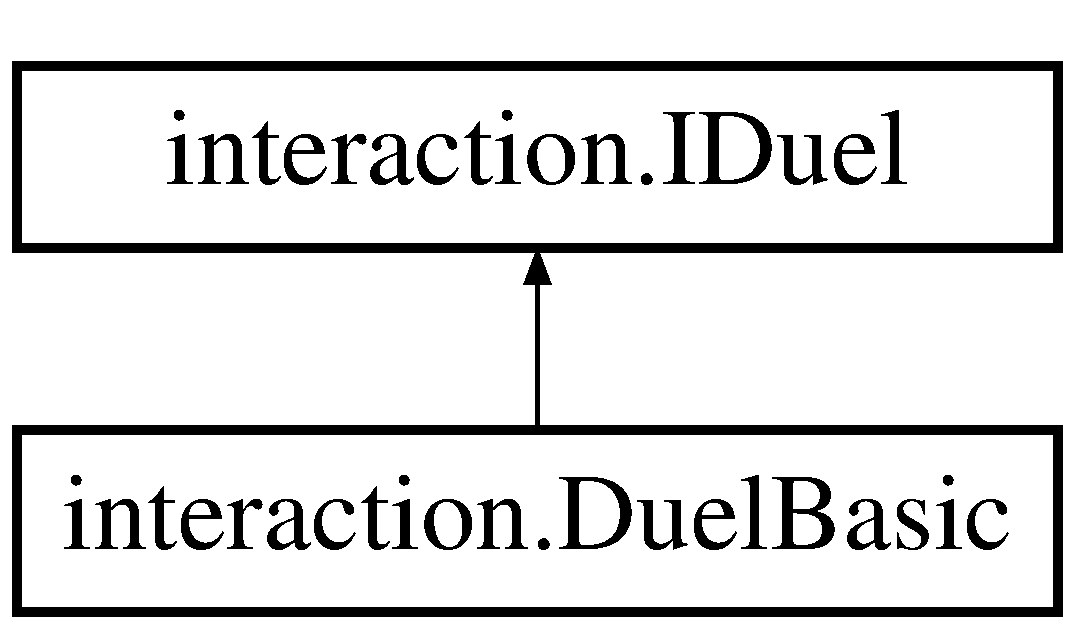
\includegraphics[height=2.000000cm]{interfaceinteraction_1_1_i_duel}
\end{center}
\end{figure}
\subsection*{Public Member Functions}
\begin{DoxyCompactItemize}
\item 
int \hyperlink{interfaceinteraction_1_1_i_duel_a33a6e184f490717f27bed44b649814be}{realiser\-Combat} ()  throws Remote\-Exception
\item 
Remote \hyperlink{interfaceinteraction_1_1_i_duel_a17fc4fd253c7e9a02f3e0edf7680e67f}{get\-Ref\-Attaquant} ()  throws Remote\-Exception
\item 
Remote \hyperlink{interfaceinteraction_1_1_i_duel_abc31afdeab5a1251c28bd6e61e828fe1}{get\-Ref\-Defenseur} ()  throws Remote\-Exception
\end{DoxyCompactItemize}


\subsection{Member Function Documentation}
\hypertarget{interfaceinteraction_1_1_i_duel_a17fc4fd253c7e9a02f3e0edf7680e67f}{\index{interaction\-::\-I\-Duel@{interaction\-::\-I\-Duel}!get\-Ref\-Attaquant@{get\-Ref\-Attaquant}}
\index{get\-Ref\-Attaquant@{get\-Ref\-Attaquant}!interaction::IDuel@{interaction\-::\-I\-Duel}}
\subsubsection[{get\-Ref\-Attaquant}]{\setlength{\rightskip}{0pt plus 5cm}Remote interaction.\-I\-Duel.\-get\-Ref\-Attaquant (
\begin{DoxyParamCaption}
{}
\end{DoxyParamCaption}
)  throws Remote\-Exception}}\label{interfaceinteraction_1_1_i_duel_a17fc4fd253c7e9a02f3e0edf7680e67f}
Renvoie la reference de l'attaquant connue par le serveur 
\begin{DoxyExceptions}{Exceptions}
{\em Remote\-Exception} & \\
\hline
\end{DoxyExceptions}


Implemented in \hyperlink{classinteraction_1_1_duel_basic_a406cd53e1eb8b51d99bbe8af72fb28d0}{interaction.\-Duel\-Basic}.

\hypertarget{interfaceinteraction_1_1_i_duel_abc31afdeab5a1251c28bd6e61e828fe1}{\index{interaction\-::\-I\-Duel@{interaction\-::\-I\-Duel}!get\-Ref\-Defenseur@{get\-Ref\-Defenseur}}
\index{get\-Ref\-Defenseur@{get\-Ref\-Defenseur}!interaction::IDuel@{interaction\-::\-I\-Duel}}
\subsubsection[{get\-Ref\-Defenseur}]{\setlength{\rightskip}{0pt plus 5cm}Remote interaction.\-I\-Duel.\-get\-Ref\-Defenseur (
\begin{DoxyParamCaption}
{}
\end{DoxyParamCaption}
)  throws Remote\-Exception}}\label{interfaceinteraction_1_1_i_duel_abc31afdeab5a1251c28bd6e61e828fe1}
Renvoie la reference du defenseur connue patr le serveur 
\begin{DoxyExceptions}{Exceptions}
{\em Remote\-Exception} & \\
\hline
\end{DoxyExceptions}


Implemented in \hyperlink{classinteraction_1_1_duel_basic_a6e7e4b0163230f13aad5ca285f969b6f}{interaction.\-Duel\-Basic}.

\hypertarget{interfaceinteraction_1_1_i_duel_a33a6e184f490717f27bed44b649814be}{\index{interaction\-::\-I\-Duel@{interaction\-::\-I\-Duel}!realiser\-Combat@{realiser\-Combat}}
\index{realiser\-Combat@{realiser\-Combat}!interaction::IDuel@{interaction\-::\-I\-Duel}}
\subsubsection[{realiser\-Combat}]{\setlength{\rightskip}{0pt plus 5cm}int interaction.\-I\-Duel.\-realiser\-Combat (
\begin{DoxyParamCaption}
{}
\end{DoxyParamCaption}
)  throws Remote\-Exception}}\label{interfaceinteraction_1_1_i_duel_a33a6e184f490717f27bed44b649814be}
Realise le combat entre deux personnages 
\begin{DoxyExceptions}{Exceptions}
{\em Remote\-Exception} & \\
\hline
\end{DoxyExceptions}


Implemented in \hyperlink{classinteraction_1_1_duel_basic_a88b42733ab5e32f5334f1c590a6dcd72}{interaction.\-Duel\-Basic}.



The documentation for this interface was generated from the following file\-:\begin{DoxyCompactItemize}
\item 
src/interaction/I\-Duel.\-java\end{DoxyCompactItemize}

\hypertarget{interfaceindividu_1_1_i_element}{\section{individu.\-I\-Element Interface Reference}
\label{interfaceindividu_1_1_i_element}\index{individu.\-I\-Element@{individu.\-I\-Element}}
}
Inheritance diagram for individu.\-I\-Element\-:\begin{figure}[H]
\begin{center}
\leavevmode
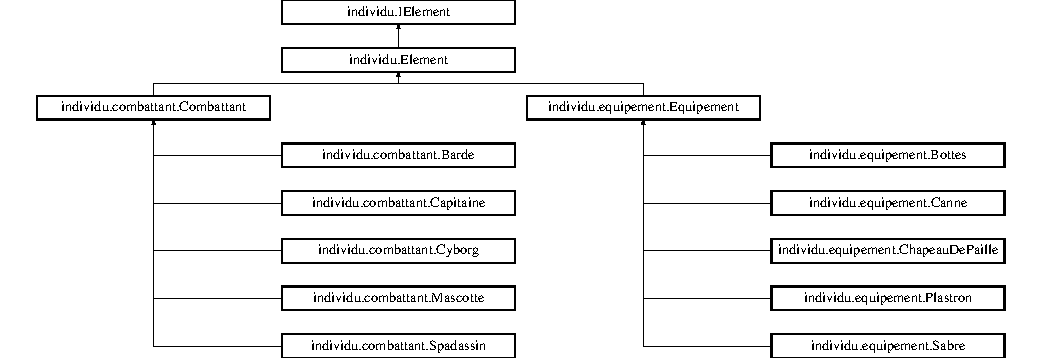
\includegraphics[height=2.000000cm]{interfaceindividu_1_1_i_element}
\end{center}
\end{figure}
\subsection*{Public Member Functions}
\begin{DoxyCompactItemize}
\item 
String \hyperlink{interfaceindividu_1_1_i_element_a7783ed1b115d522ddd6a8a0c2aded632}{get\-Nom} ()
\item 
int \hyperlink{interfaceindividu_1_1_i_element_a2f5272cb7b7f334bb9352cc2010c0abe}{get\-Vie} ()
\item 
void \hyperlink{interfaceindividu_1_1_i_element_a386d0b896afaf5481da8c6f667b11297}{set\-Vie} (int vie)
\item 
Array\-List$<$ Integer $>$ \hyperlink{interfaceindividu_1_1_i_element_abb2ad9e31a3500c3c4deaaf58f9e01c9}{get\-Elements\-Connus} ()
\item 
void \hyperlink{interfaceindividu_1_1_i_element_a8c265785d6fb0f25cc54ec5850c602d3}{ajouter\-Connu} (int ref)
\item 
String \hyperlink{interfaceindividu_1_1_i_element_a4609baa01e8f8558e931b2f8901e789d}{to\-String} ()
\end{DoxyCompactItemize}


\subsection{Member Function Documentation}
\hypertarget{interfaceindividu_1_1_i_element_a8c265785d6fb0f25cc54ec5850c602d3}{\index{individu\-::\-I\-Element@{individu\-::\-I\-Element}!ajouter\-Connu@{ajouter\-Connu}}
\index{ajouter\-Connu@{ajouter\-Connu}!individu::IElement@{individu\-::\-I\-Element}}
\subsubsection[{ajouter\-Connu}]{\setlength{\rightskip}{0pt plus 5cm}void individu.\-I\-Element.\-ajouter\-Connu (
\begin{DoxyParamCaption}
\item[{int}]{ref}
\end{DoxyParamCaption}
)}}\label{interfaceindividu_1_1_i_element_a8c265785d6fb0f25cc54ec5850c602d3}
Ajoute a la liste des elements connus (elements avec lesquels l'objet courant a joue) un nouvel element 
\begin{DoxyParams}{Parameters}
{\em ref} & le reference de l'objet avec qui il joue \\
\hline
\end{DoxyParams}


Implemented in \hyperlink{classindividu_1_1_element_aaaa713cc814adae8a8dda825263b48db}{individu.\-Element}.

\hypertarget{interfaceindividu_1_1_i_element_abb2ad9e31a3500c3c4deaaf58f9e01c9}{\index{individu\-::\-I\-Element@{individu\-::\-I\-Element}!get\-Elements\-Connus@{get\-Elements\-Connus}}
\index{get\-Elements\-Connus@{get\-Elements\-Connus}!individu::IElement@{individu\-::\-I\-Element}}
\subsubsection[{get\-Elements\-Connus}]{\setlength{\rightskip}{0pt plus 5cm}Array\-List$<$Integer$>$ individu.\-I\-Element.\-get\-Elements\-Connus (
\begin{DoxyParamCaption}
{}
\end{DoxyParamCaption}
)}}\label{interfaceindividu_1_1_i_element_abb2ad9e31a3500c3c4deaaf58f9e01c9}
\begin{DoxyVerb}Retourne les references des elements avec lesquels l'element courant a joue
\end{DoxyVerb}
 \begin{DoxyReturn}{Returns}

\end{DoxyReturn}


Implemented in \hyperlink{classindividu_1_1_element_a46430a36f795bf42832317f96fdeeb5e}{individu.\-Element}.

\hypertarget{interfaceindividu_1_1_i_element_a7783ed1b115d522ddd6a8a0c2aded632}{\index{individu\-::\-I\-Element@{individu\-::\-I\-Element}!get\-Nom@{get\-Nom}}
\index{get\-Nom@{get\-Nom}!individu::IElement@{individu\-::\-I\-Element}}
\subsubsection[{get\-Nom}]{\setlength{\rightskip}{0pt plus 5cm}String individu.\-I\-Element.\-get\-Nom (
\begin{DoxyParamCaption}
{}
\end{DoxyParamCaption}
)}}\label{interfaceindividu_1_1_i_element_a7783ed1b115d522ddd6a8a0c2aded632}
\begin{DoxyVerb}Retourne le nom de l'element
\end{DoxyVerb}
 \begin{DoxyReturn}{Returns}

\end{DoxyReturn}


Implemented in \hyperlink{classindividu_1_1_element_a2623a37998d1558ad9d9f9352f833cd4}{individu.\-Element}.

\hypertarget{interfaceindividu_1_1_i_element_a2f5272cb7b7f334bb9352cc2010c0abe}{\index{individu\-::\-I\-Element@{individu\-::\-I\-Element}!get\-Vie@{get\-Vie}}
\index{get\-Vie@{get\-Vie}!individu::IElement@{individu\-::\-I\-Element}}
\subsubsection[{get\-Vie}]{\setlength{\rightskip}{0pt plus 5cm}int individu.\-I\-Element.\-get\-Vie (
\begin{DoxyParamCaption}
{}
\end{DoxyParamCaption}
)}}\label{interfaceindividu_1_1_i_element_a2f5272cb7b7f334bb9352cc2010c0abe}
\begin{DoxyVerb}Retourne le nombre de vies de l'element
\end{DoxyVerb}
 \begin{DoxyReturn}{Returns}

\end{DoxyReturn}


Implemented in \hyperlink{classindividu_1_1_element_ab41f49b096712f65285de4437f1b15b5}{individu.\-Element}.

\hypertarget{interfaceindividu_1_1_i_element_a386d0b896afaf5481da8c6f667b11297}{\index{individu\-::\-I\-Element@{individu\-::\-I\-Element}!set\-Vie@{set\-Vie}}
\index{set\-Vie@{set\-Vie}!individu::IElement@{individu\-::\-I\-Element}}
\subsubsection[{set\-Vie}]{\setlength{\rightskip}{0pt plus 5cm}void individu.\-I\-Element.\-set\-Vie (
\begin{DoxyParamCaption}
\item[{int}]{vie}
\end{DoxyParamCaption}
)}}\label{interfaceindividu_1_1_i_element_a386d0b896afaf5481da8c6f667b11297}
Reinitialise le nombre de vies de l'element 
\begin{DoxyParams}{Parameters}
{\em vie} & le nouveau nombre de vie \\
\hline
\end{DoxyParams}


Implemented in \hyperlink{classindividu_1_1_element_ad8c8123352986a7e80dea748e34922cc}{individu.\-Element}.

\hypertarget{interfaceindividu_1_1_i_element_a4609baa01e8f8558e931b2f8901e789d}{\index{individu\-::\-I\-Element@{individu\-::\-I\-Element}!to\-String@{to\-String}}
\index{to\-String@{to\-String}!individu::IElement@{individu\-::\-I\-Element}}
\subsubsection[{to\-String}]{\setlength{\rightskip}{0pt plus 5cm}String individu.\-I\-Element.\-to\-String (
\begin{DoxyParamCaption}
{}
\end{DoxyParamCaption}
)}}\label{interfaceindividu_1_1_i_element_a4609baa01e8f8558e931b2f8901e789d}
Renvoie les informations concernant l'element courant \begin{DoxyReturn}{Returns}
chaine de caractere contenant au moins le nom de l'element et le nombre de vies tel qu'il sera affiche sur l'interface graphique 
\end{DoxyReturn}


Implemented in \hyperlink{classindividu_1_1_element_af4c2b08d92cfad7532168a5ccd6c2ebb}{individu.\-Element}.



The documentation for this interface was generated from the following file\-:\begin{DoxyCompactItemize}
\item 
src/individu/I\-Element.\-java\end{DoxyCompactItemize}

\hypertarget{classinterface_graphique_1_1_i_h_m}{\section{interface\-Graphique.\-I\-H\-M Class Reference}
\label{classinterface_graphique_1_1_i_h_m}\index{interface\-Graphique.\-I\-H\-M@{interface\-Graphique.\-I\-H\-M}}
}


Inherits J\-Frame.

\subsection*{Classes}
\begin{DoxyCompactItemize}
\item 
class {\bfseries Arene\-J\-Panel}
\item 
class {\bfseries Arene\-J\-Text\-Area}
\item 
enum {\bfseries State}
\end{DoxyCompactItemize}
\subsection*{Public Member Functions}
\begin{DoxyCompactItemize}
\item 
void \hyperlink{classinterface_graphique_1_1_i_h_m_aad37d96bab73c365d6f654352ff0ec71}{connect} ()
\end{DoxyCompactItemize}


\subsection{Member Function Documentation}
\hypertarget{classinterface_graphique_1_1_i_h_m_aad37d96bab73c365d6f654352ff0ec71}{\index{interface\-Graphique\-::\-I\-H\-M@{interface\-Graphique\-::\-I\-H\-M}!connect@{connect}}
\index{connect@{connect}!interfaceGraphique::IHM@{interface\-Graphique\-::\-I\-H\-M}}
\subsubsection[{connect}]{\setlength{\rightskip}{0pt plus 5cm}void interface\-Graphique.\-I\-H\-M.\-connect (
\begin{DoxyParamCaption}
{}
\end{DoxyParamCaption}
)}}\label{classinterface_graphique_1_1_i_h_m_aad37d96bab73c365d6f654352ff0ec71}
Lance une connexion au serveur dans un thread separe 

The documentation for this class was generated from the following file\-:\begin{DoxyCompactItemize}
\item 
src/interface\-Graphique/I\-H\-M.\-java\end{DoxyCompactItemize}

\hypertarget{classindividu_1_1combattant_1_1_liste_equipements}{\section{Référence de la classe individu.\-combattant.\-Liste\-Equipements}
\label{classindividu_1_1combattant_1_1_liste_equipements}\index{individu.\-combattant.\-Liste\-Equipements@{individu.\-combattant.\-Liste\-Equipements}}
}


Est dérivée de Array\-List$<$ Equipement $>$.

\subsection*{Fonctions membres publiques}
\begin{DoxyCompactItemize}
\item 
\hyperlink{classindividu_1_1combattant_1_1_liste_equipements_a7504b743eea66dd791f726abd0ce001d}{Liste\-Equipements} (final int p\-Nb\-Max\-Eq)
\item 
boolean \hyperlink{classindividu_1_1combattant_1_1_liste_equipements_a0c42c384b01ae1bee9f699e3ac982a4c}{add} (\hyperlink{classindividu_1_1equipement_1_1_equipement}{Equipement} p\-Eleme)
\item 
boolean \hyperlink{classindividu_1_1combattant_1_1_liste_equipements_a5b256703d5a9cef1deb013eff6ae34ff}{nb\-Max\-Atteind} ()
\item 
int \hyperlink{classindividu_1_1combattant_1_1_liste_equipements_a5b9385493928dd0a8d3d508b4f906e51}{get\-Somme\-Attaque} ()
\item 
int \hyperlink{classindividu_1_1combattant_1_1_liste_equipements_af7f605713d45e20433c34de1d27561b3}{get\-Somme\-Defense} ()
\item 
int \hyperlink{classindividu_1_1combattant_1_1_liste_equipements_aef396dda965399ad7f729bd9fa013392}{get\-Somme\-Vitesse} ()
\item 
int \hyperlink{classindividu_1_1combattant_1_1_liste_equipements_ae92d592c6d61c7a767f66e51118b9afa}{duree\-Apres\-Combat} ()
\item 
int \hyperlink{classindividu_1_1combattant_1_1_liste_equipements_abe918cd79ec7bc71655efbcdf320d86a}{get\-Nb\-Max\-Eq} ()
\item 
void \hyperlink{classindividu_1_1combattant_1_1_liste_equipements_a4ad481963d8b9c35a0994522c506bd48}{set\-Nb\-Max\-Eq} (int p\-Nb\-Max\-Eq)
\end{DoxyCompactItemize}


\subsection{Description détaillée}
Collection d'équipement possédant une valeur maximum d'élément. 

\subsection{Documentation des constructeurs et destructeur}
\hypertarget{classindividu_1_1combattant_1_1_liste_equipements_a7504b743eea66dd791f726abd0ce001d}{\index{individu\-::combattant\-::\-Liste\-Equipements@{individu\-::combattant\-::\-Liste\-Equipements}!Liste\-Equipements@{Liste\-Equipements}}
\index{Liste\-Equipements@{Liste\-Equipements}!individu::combattant::ListeEquipements@{individu\-::combattant\-::\-Liste\-Equipements}}
\subsubsection[{Liste\-Equipements}]{\setlength{\rightskip}{0pt plus 5cm}individu.\-combattant.\-Liste\-Equipements.\-Liste\-Equipements (
\begin{DoxyParamCaption}
\item[{final int}]{p\-Nb\-Max\-Eq}
\end{DoxyParamCaption}
)}}\label{classindividu_1_1combattant_1_1_liste_equipements_a7504b743eea66dd791f726abd0ce001d}
Constructeur 
\begin{DoxyParams}{Paramètres}
{\em p\-Nb\-Max\-Eq} & Initialisation du nombre max d'équipement \\
\hline
\end{DoxyParams}


\subsection{Documentation des fonctions membres}
\hypertarget{classindividu_1_1combattant_1_1_liste_equipements_a0c42c384b01ae1bee9f699e3ac982a4c}{\index{individu\-::combattant\-::\-Liste\-Equipements@{individu\-::combattant\-::\-Liste\-Equipements}!add@{add}}
\index{add@{add}!individu::combattant::ListeEquipements@{individu\-::combattant\-::\-Liste\-Equipements}}
\subsubsection[{add}]{\setlength{\rightskip}{0pt plus 5cm}boolean individu.\-combattant.\-Liste\-Equipements.\-add (
\begin{DoxyParamCaption}
\item[{{\bf Equipement}}]{p\-Eleme}
\end{DoxyParamCaption}
)}}\label{classindividu_1_1combattant_1_1_liste_equipements_a0c42c384b01ae1bee9f699e3ac982a4c}
Ajoute un nouvel équipement 
\begin{DoxyParams}{Paramètres}
{\em p\-Eleme} & L'élément à ajouter \\
\hline
\end{DoxyParams}
\begin{DoxyReturn}{Renvoie}
true si l'élément à été ajouté, 0 si le nombre max est atteind ou si une erreur s'est produite. 
\end{DoxyReturn}
\hypertarget{classindividu_1_1combattant_1_1_liste_equipements_ae92d592c6d61c7a767f66e51118b9afa}{\index{individu\-::combattant\-::\-Liste\-Equipements@{individu\-::combattant\-::\-Liste\-Equipements}!duree\-Apres\-Combat@{duree\-Apres\-Combat}}
\index{duree\-Apres\-Combat@{duree\-Apres\-Combat}!individu::combattant::ListeEquipements@{individu\-::combattant\-::\-Liste\-Equipements}}
\subsubsection[{duree\-Apres\-Combat}]{\setlength{\rightskip}{0pt plus 5cm}int individu.\-combattant.\-Liste\-Equipements.\-duree\-Apres\-Combat (
\begin{DoxyParamCaption}
{}
\end{DoxyParamCaption}
)}}\label{classindividu_1_1combattant_1_1_liste_equipements_ae92d592c6d61c7a767f66e51118b9afa}
Retourne la durée d'un équipement après le combat. Si la durée atteind 0, alors l'équipement est détruis de la liste.

\begin{DoxyReturn}{Renvoie}
La nouvelle durée 
\end{DoxyReturn}
\hypertarget{classindividu_1_1combattant_1_1_liste_equipements_abe918cd79ec7bc71655efbcdf320d86a}{\index{individu\-::combattant\-::\-Liste\-Equipements@{individu\-::combattant\-::\-Liste\-Equipements}!get\-Nb\-Max\-Eq@{get\-Nb\-Max\-Eq}}
\index{get\-Nb\-Max\-Eq@{get\-Nb\-Max\-Eq}!individu::combattant::ListeEquipements@{individu\-::combattant\-::\-Liste\-Equipements}}
\subsubsection[{get\-Nb\-Max\-Eq}]{\setlength{\rightskip}{0pt plus 5cm}int individu.\-combattant.\-Liste\-Equipements.\-get\-Nb\-Max\-Eq (
\begin{DoxyParamCaption}
{}
\end{DoxyParamCaption}
)}}\label{classindividu_1_1combattant_1_1_liste_equipements_abe918cd79ec7bc71655efbcdf320d86a}
Retourne le nombre maxium d'équipement possible \begin{DoxyReturn}{Renvoie}
La nombre d'équipement 
\end{DoxyReturn}
\hypertarget{classindividu_1_1combattant_1_1_liste_equipements_a5b9385493928dd0a8d3d508b4f906e51}{\index{individu\-::combattant\-::\-Liste\-Equipements@{individu\-::combattant\-::\-Liste\-Equipements}!get\-Somme\-Attaque@{get\-Somme\-Attaque}}
\index{get\-Somme\-Attaque@{get\-Somme\-Attaque}!individu::combattant::ListeEquipements@{individu\-::combattant\-::\-Liste\-Equipements}}
\subsubsection[{get\-Somme\-Attaque}]{\setlength{\rightskip}{0pt plus 5cm}int individu.\-combattant.\-Liste\-Equipements.\-get\-Somme\-Attaque (
\begin{DoxyParamCaption}
{}
\end{DoxyParamCaption}
)}}\label{classindividu_1_1combattant_1_1_liste_equipements_a5b9385493928dd0a8d3d508b4f906e51}
Retourne la somme du bonus d'attaque des équipements de la lite. \begin{DoxyReturn}{Renvoie}
La somme d'attaque 
\end{DoxyReturn}
\hypertarget{classindividu_1_1combattant_1_1_liste_equipements_af7f605713d45e20433c34de1d27561b3}{\index{individu\-::combattant\-::\-Liste\-Equipements@{individu\-::combattant\-::\-Liste\-Equipements}!get\-Somme\-Defense@{get\-Somme\-Defense}}
\index{get\-Somme\-Defense@{get\-Somme\-Defense}!individu::combattant::ListeEquipements@{individu\-::combattant\-::\-Liste\-Equipements}}
\subsubsection[{get\-Somme\-Defense}]{\setlength{\rightskip}{0pt plus 5cm}int individu.\-combattant.\-Liste\-Equipements.\-get\-Somme\-Defense (
\begin{DoxyParamCaption}
{}
\end{DoxyParamCaption}
)}}\label{classindividu_1_1combattant_1_1_liste_equipements_af7f605713d45e20433c34de1d27561b3}
Retourne la somme du bonus de défense des équipements de la liste. \begin{DoxyReturn}{Renvoie}
La somme d'attaque 
\end{DoxyReturn}
\hypertarget{classindividu_1_1combattant_1_1_liste_equipements_aef396dda965399ad7f729bd9fa013392}{\index{individu\-::combattant\-::\-Liste\-Equipements@{individu\-::combattant\-::\-Liste\-Equipements}!get\-Somme\-Vitesse@{get\-Somme\-Vitesse}}
\index{get\-Somme\-Vitesse@{get\-Somme\-Vitesse}!individu::combattant::ListeEquipements@{individu\-::combattant\-::\-Liste\-Equipements}}
\subsubsection[{get\-Somme\-Vitesse}]{\setlength{\rightskip}{0pt plus 5cm}int individu.\-combattant.\-Liste\-Equipements.\-get\-Somme\-Vitesse (
\begin{DoxyParamCaption}
{}
\end{DoxyParamCaption}
)}}\label{classindividu_1_1combattant_1_1_liste_equipements_aef396dda965399ad7f729bd9fa013392}
Retourne la somme du bonus de vitesse des équipements de la liste. \begin{DoxyReturn}{Renvoie}
La somme d'attaque 
\end{DoxyReturn}
\hypertarget{classindividu_1_1combattant_1_1_liste_equipements_a5b256703d5a9cef1deb013eff6ae34ff}{\index{individu\-::combattant\-::\-Liste\-Equipements@{individu\-::combattant\-::\-Liste\-Equipements}!nb\-Max\-Atteind@{nb\-Max\-Atteind}}
\index{nb\-Max\-Atteind@{nb\-Max\-Atteind}!individu::combattant::ListeEquipements@{individu\-::combattant\-::\-Liste\-Equipements}}
\subsubsection[{nb\-Max\-Atteind}]{\setlength{\rightskip}{0pt plus 5cm}boolean individu.\-combattant.\-Liste\-Equipements.\-nb\-Max\-Atteind (
\begin{DoxyParamCaption}
{}
\end{DoxyParamCaption}
)}}\label{classindividu_1_1combattant_1_1_liste_equipements_a5b256703d5a9cef1deb013eff6ae34ff}
Retourne si le nombre max d'équipement est atteind ou non. \begin{DoxyReturn}{Renvoie}
vrai si le nombre max d'équipement est atteind, faux sinon. 
\end{DoxyReturn}
\hypertarget{classindividu_1_1combattant_1_1_liste_equipements_a4ad481963d8b9c35a0994522c506bd48}{\index{individu\-::combattant\-::\-Liste\-Equipements@{individu\-::combattant\-::\-Liste\-Equipements}!set\-Nb\-Max\-Eq@{set\-Nb\-Max\-Eq}}
\index{set\-Nb\-Max\-Eq@{set\-Nb\-Max\-Eq}!individu::combattant::ListeEquipements@{individu\-::combattant\-::\-Liste\-Equipements}}
\subsubsection[{set\-Nb\-Max\-Eq}]{\setlength{\rightskip}{0pt plus 5cm}void individu.\-combattant.\-Liste\-Equipements.\-set\-Nb\-Max\-Eq (
\begin{DoxyParamCaption}
\item[{int}]{p\-Nb\-Max\-Eq}
\end{DoxyParamCaption}
)}}\label{classindividu_1_1combattant_1_1_liste_equipements_a4ad481963d8b9c35a0994522c506bd48}
Réinitialise le nombre d'équipement maximum 
\begin{DoxyParams}{Paramètres}
{\em p\-Nb\-Max\-Eq} & Le nouveau nombre maximum d'équipement \\
\hline
\end{DoxyParams}


La documentation de cette classe a été générée à partir du fichier suivant \-:\begin{DoxyCompactItemize}
\item 
src/individu/combattant/Liste\-Equipements.\-java\end{DoxyCompactItemize}

\hypertarget{classindividu_1_1combattant_1_1_mascotte}{\section{Référence de la classe individu.\-combattant.\-Mascotte}
\label{classindividu_1_1combattant_1_1_mascotte}\index{individu.\-combattant.\-Mascotte@{individu.\-combattant.\-Mascotte}}
}
Graphe d'héritage de individu.\-combattant.\-Mascotte\-:\begin{figure}[H]
\begin{center}
\leavevmode
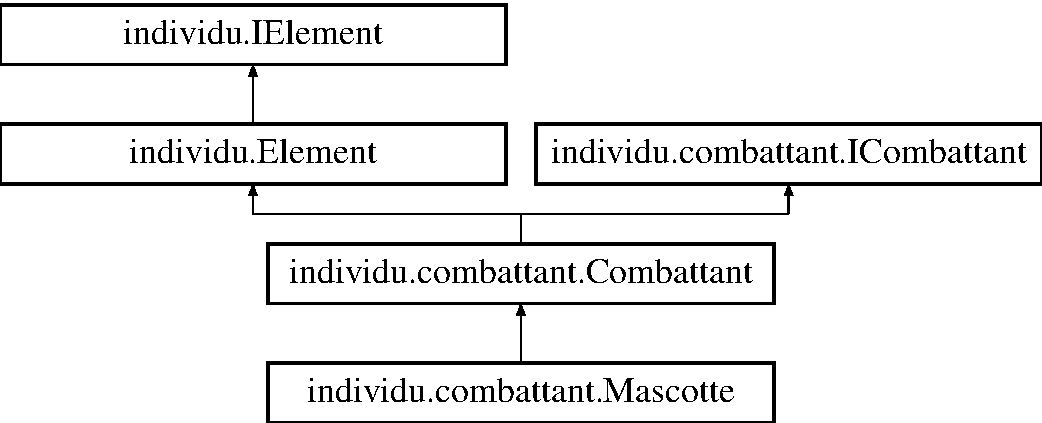
\includegraphics[height=4.000000cm]{classindividu_1_1combattant_1_1_mascotte}
\end{center}
\end{figure}
\subsection*{Fonctions membres publiques}
\begin{DoxyCompactItemize}
\item 
\hyperlink{classindividu_1_1combattant_1_1_mascotte_ae2d5f7e55cf9a0dcb2007ceb3c038911}{Mascotte} (String nom)
\end{DoxyCompactItemize}
\subsection*{Additional Inherited Members}


\subsection{Description détaillée}
Initialise un \hyperlink{classindividu_1_1combattant_1_1_combattant}{Combattant} avec les capacités d'une \hyperlink{classindividu_1_1combattant_1_1_mascotte}{Mascotte} 

\subsection{Documentation des constructeurs et destructeur}
\hypertarget{classindividu_1_1combattant_1_1_mascotte_ae2d5f7e55cf9a0dcb2007ceb3c038911}{\index{individu\-::combattant\-::\-Mascotte@{individu\-::combattant\-::\-Mascotte}!Mascotte@{Mascotte}}
\index{Mascotte@{Mascotte}!individu::combattant::Mascotte@{individu\-::combattant\-::\-Mascotte}}
\subsubsection[{Mascotte}]{\setlength{\rightskip}{0pt plus 5cm}individu.\-combattant.\-Mascotte.\-Mascotte (
\begin{DoxyParamCaption}
\item[{String}]{nom}
\end{DoxyParamCaption}
)}}\label{classindividu_1_1combattant_1_1_mascotte_ae2d5f7e55cf9a0dcb2007ceb3c038911}
Constructeur 
\begin{DoxyParams}{Paramètres}
{\em nom} & Le nom du \hyperlink{classindividu_1_1combattant_1_1_mascotte}{Mascotte} \\
\hline
\end{DoxyParams}


La documentation de cette classe a été générée à partir du fichier suivant \-:\begin{DoxyCompactItemize}
\item 
src/individu/combattant/Mascotte.\-java\end{DoxyCompactItemize}

\hypertarget{classindividu_1_1equipement_1_1_plastron}{\section{Référence de la classe individu.\-equipement.\-Plastron}
\label{classindividu_1_1equipement_1_1_plastron}\index{individu.\-equipement.\-Plastron@{individu.\-equipement.\-Plastron}}
}
Graphe d'héritage de individu.\-equipement.\-Plastron\-:\begin{figure}[H]
\begin{center}
\leavevmode
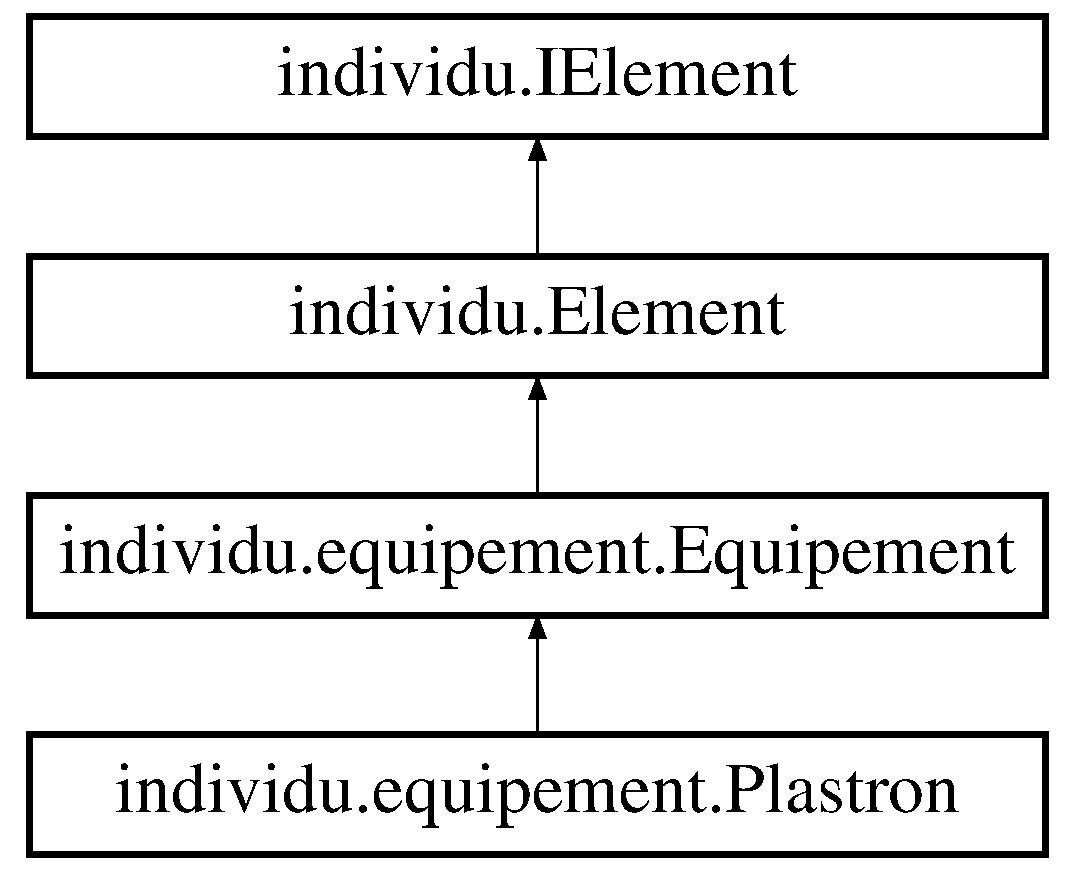
\includegraphics[height=4.000000cm]{classindividu_1_1equipement_1_1_plastron}
\end{center}
\end{figure}
\subsection*{Fonctions membres publiques}
\begin{DoxyCompactItemize}
\item 
\hypertarget{classindividu_1_1equipement_1_1_plastron_ac95f0733dbb08cf0ad3af4dba28c90fe}{{\bfseries Plastron} (String nom)}\label{classindividu_1_1equipement_1_1_plastron_ac95f0733dbb08cf0ad3af4dba28c90fe}

\end{DoxyCompactItemize}


\subsection{Description détaillée}
Initialise un équipement avec les capacités d'un plastron 

La documentation de cette classe a été générée à partir du fichier suivant \-:\begin{DoxyCompactItemize}
\item 
src/individu/equipement/Plastron.\-java\end{DoxyCompactItemize}

\hypertarget{classinterface_graphique_1_1_point_comp}{\section{interface\-Graphique.\-Point\-Comp Class Reference}
\label{classinterface_graphique_1_1_point_comp}\index{interface\-Graphique.\-Point\-Comp@{interface\-Graphique.\-Point\-Comp}}
}


Inherits Point, and Comparator$<$ Point $>$.

\subsection*{Public Member Functions}
\begin{DoxyCompactItemize}
\item 
\hyperlink{classinterface_graphique_1_1_point_comp_a445b387040f356ab15230221389ecddf}{Point\-Comp} (int x, int y)
\item 
\hyperlink{classinterface_graphique_1_1_point_comp_af60c856a56ce03b321d589f5d691ba8c}{Point\-Comp} (Point objectif)
\item 
int \hyperlink{classinterface_graphique_1_1_point_comp_aaaa8644250b70b34ee1a86da23e14a3a}{compare} (Point o1, Point o2)
\end{DoxyCompactItemize}


\subsection{Constructor \& Destructor Documentation}
\hypertarget{classinterface_graphique_1_1_point_comp_a445b387040f356ab15230221389ecddf}{\index{interface\-Graphique\-::\-Point\-Comp@{interface\-Graphique\-::\-Point\-Comp}!Point\-Comp@{Point\-Comp}}
\index{Point\-Comp@{Point\-Comp}!interfaceGraphique::PointComp@{interface\-Graphique\-::\-Point\-Comp}}
\subsubsection[{Point\-Comp}]{\setlength{\rightskip}{0pt plus 5cm}interface\-Graphique.\-Point\-Comp.\-Point\-Comp (
\begin{DoxyParamCaption}
\item[{int}]{x, }
\item[{int}]{y}
\end{DoxyParamCaption}
)}}\label{classinterface_graphique_1_1_point_comp_a445b387040f356ab15230221389ecddf}
Constructeur 
\begin{DoxyParams}{Parameters}
{\em x} & la valeur de l'ordonnee \\
\hline
{\em y} & la valeur de l'abscisse \\
\hline
\end{DoxyParams}
\hypertarget{classinterface_graphique_1_1_point_comp_af60c856a56ce03b321d589f5d691ba8c}{\index{interface\-Graphique\-::\-Point\-Comp@{interface\-Graphique\-::\-Point\-Comp}!Point\-Comp@{Point\-Comp}}
\index{Point\-Comp@{Point\-Comp}!interfaceGraphique::PointComp@{interface\-Graphique\-::\-Point\-Comp}}
\subsubsection[{Point\-Comp}]{\setlength{\rightskip}{0pt plus 5cm}interface\-Graphique.\-Point\-Comp.\-Point\-Comp (
\begin{DoxyParamCaption}
\item[{Point}]{objectif}
\end{DoxyParamCaption}
)}}\label{classinterface_graphique_1_1_point_comp_af60c856a56ce03b321d589f5d691ba8c}
Constructeur 
\begin{DoxyParams}{Parameters}
{\em objectif} & le point \\
\hline
\end{DoxyParams}


\subsection{Member Function Documentation}
\hypertarget{classinterface_graphique_1_1_point_comp_aaaa8644250b70b34ee1a86da23e14a3a}{\index{interface\-Graphique\-::\-Point\-Comp@{interface\-Graphique\-::\-Point\-Comp}!compare@{compare}}
\index{compare@{compare}!interfaceGraphique::PointComp@{interface\-Graphique\-::\-Point\-Comp}}
\subsubsection[{compare}]{\setlength{\rightskip}{0pt plus 5cm}int interface\-Graphique.\-Point\-Comp.\-compare (
\begin{DoxyParamCaption}
\item[{Point}]{o1, }
\item[{Point}]{o2}
\end{DoxyParamCaption}
)}}\label{classinterface_graphique_1_1_point_comp_aaaa8644250b70b34ee1a86da23e14a3a}
Compare la distance de l'objet courant a deux autres points 
\begin{DoxyParams}{Parameters}
{\em o1} & le premier point \\
\hline
{\em o2} & le deuxieme point \\
\hline
\end{DoxyParams}
\begin{DoxyReturn}{Returns}
$<$0 si le premier point est plus proche, 0 si les points sont a la meme distance et 1 si le deuxieme est plus proche 
\end{DoxyReturn}


The documentation for this class was generated from the following file\-:\begin{DoxyCompactItemize}
\item 
src/interface\-Graphique/Point\-Comp.\-java\end{DoxyCompactItemize}

\hypertarget{classindividu_1_1equipement_1_1_sabre}{\section{Référence de la classe individu.\-equipement.\-Sabre}
\label{classindividu_1_1equipement_1_1_sabre}\index{individu.\-equipement.\-Sabre@{individu.\-equipement.\-Sabre}}
}
Graphe d'héritage de individu.\-equipement.\-Sabre\-:\begin{figure}[H]
\begin{center}
\leavevmode
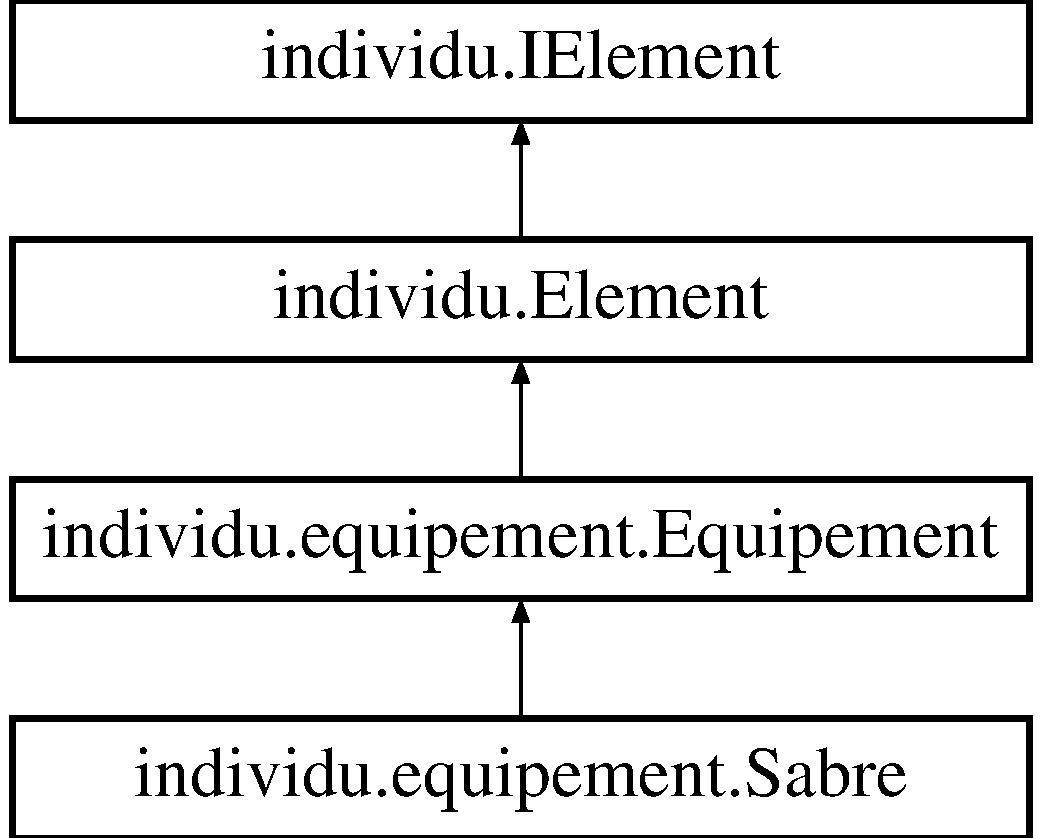
\includegraphics[height=4.000000cm]{classindividu_1_1equipement_1_1_sabre}
\end{center}
\end{figure}
\subsection*{Fonctions membres publiques}
\begin{DoxyCompactItemize}
\item 
\hypertarget{classindividu_1_1equipement_1_1_sabre_a0480e9c7f234f72d0453950787e0421e}{{\bfseries Sabre} (String nom)}\label{classindividu_1_1equipement_1_1_sabre_a0480e9c7f234f72d0453950787e0421e}

\end{DoxyCompactItemize}


La documentation de cette classe a été générée à partir du fichier suivant \-:\begin{DoxyCompactItemize}
\item 
src/individu/equipement/Sabre.\-java\end{DoxyCompactItemize}

\hypertarget{classindividu_1_1combattant_1_1_spadassin}{\section{Référence de la classe individu.\-combattant.\-Spadassin}
\label{classindividu_1_1combattant_1_1_spadassin}\index{individu.\-combattant.\-Spadassin@{individu.\-combattant.\-Spadassin}}
}
Graphe d'héritage de individu.\-combattant.\-Spadassin\-:\begin{figure}[H]
\begin{center}
\leavevmode
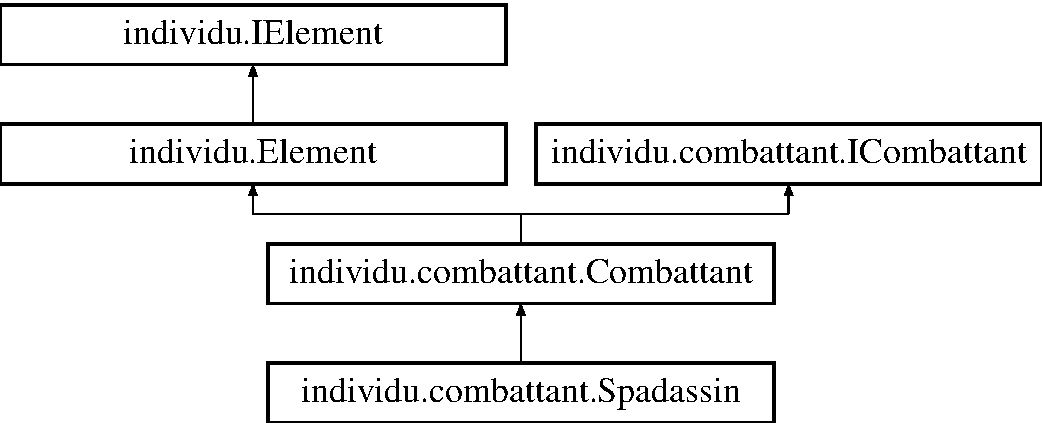
\includegraphics[height=4.000000cm]{classindividu_1_1combattant_1_1_spadassin}
\end{center}
\end{figure}
\subsection*{Fonctions membres publiques}
\begin{DoxyCompactItemize}
\item 
\hyperlink{classindividu_1_1combattant_1_1_spadassin_ac9d68ca6c6ad9760a55705e7814f47ec}{Spadassin} (String nom)
\end{DoxyCompactItemize}
\subsection*{Additional Inherited Members}


\subsection{Description détaillée}
Initialise un \hyperlink{classindividu_1_1combattant_1_1_combattant}{Combattant} avec les capacités d'un \hyperlink{classindividu_1_1combattant_1_1_spadassin}{Spadassin} 

\subsection{Documentation des constructeurs et destructeur}
\hypertarget{classindividu_1_1combattant_1_1_spadassin_ac9d68ca6c6ad9760a55705e7814f47ec}{\index{individu\-::combattant\-::\-Spadassin@{individu\-::combattant\-::\-Spadassin}!Spadassin@{Spadassin}}
\index{Spadassin@{Spadassin}!individu::combattant::Spadassin@{individu\-::combattant\-::\-Spadassin}}
\subsubsection[{Spadassin}]{\setlength{\rightskip}{0pt plus 5cm}individu.\-combattant.\-Spadassin.\-Spadassin (
\begin{DoxyParamCaption}
\item[{String}]{nom}
\end{DoxyParamCaption}
)}}\label{classindividu_1_1combattant_1_1_spadassin_ac9d68ca6c6ad9760a55705e7814f47ec}
Constructeur 
\begin{DoxyParams}{Paramètres}
{\em nom} & Le nom du \hyperlink{classindividu_1_1combattant_1_1_spadassin}{Spadassin} \\
\hline
\end{DoxyParams}


La documentation de cette classe a été générée à partir du fichier suivant \-:\begin{DoxyCompactItemize}
\item 
src/individu/combattant/Spadassin.\-java\end{DoxyCompactItemize}

\hypertarget{classcontrole_1_1_strategie}{\section{controle.\-Strategie Class Reference}
\label{classcontrole_1_1_strategie}\index{controle.\-Strategie@{controle.\-Strategie}}
}
\subsection*{Static Public Member Functions}
\begin{DoxyCompactItemize}
\item 
static Hash\-Map$<$ Integer, \\*
Hash\-Map$<$ Integer, \hyperlink{classinterface_graphique_1_1_vue_element}{Vue\-Element} $>$ $>$ \hyperlink{classcontrole_1_1_strategie_a948276367808b670e3c7af06f951eac6}{chercher\-Element\-Proche} (\hyperlink{classinterface_graphique_1_1_vue_element}{Vue\-Element} ve, Hashtable$<$ Integer, \hyperlink{classinterface_graphique_1_1_vue_element}{Vue\-Element} $>$ voisins)
\end{DoxyCompactItemize}


\subsection{Member Function Documentation}
\hypertarget{classcontrole_1_1_strategie_a948276367808b670e3c7af06f951eac6}{\index{controle\-::\-Strategie@{controle\-::\-Strategie}!chercher\-Element\-Proche@{chercher\-Element\-Proche}}
\index{chercher\-Element\-Proche@{chercher\-Element\-Proche}!controle::Strategie@{controle\-::\-Strategie}}
\subsubsection[{chercher\-Element\-Proche}]{\setlength{\rightskip}{0pt plus 5cm}static Hash\-Map$<$Integer, Hash\-Map$<$Integer,{\bf Vue\-Element}$>$ $>$ controle.\-Strategie.\-chercher\-Element\-Proche (
\begin{DoxyParamCaption}
\item[{{\bf Vue\-Element}}]{ve, }
\item[{Hashtable$<$ Integer, {\bf Vue\-Element} $>$}]{voisins}
\end{DoxyParamCaption}
)\hspace{0.3cm}{\ttfamily [static]}}}\label{classcontrole_1_1_strategie_a948276367808b670e3c7af06f951eac6}
Cherche l'element le plus proche vers lequel se diriger 
\begin{DoxyParams}{Parameters}
{\em ve} & l'element courant \\
\hline
{\em voisins} & les elements voisins \\
\hline
\end{DoxyParams}
\begin{DoxyReturn}{Returns}
un hashmap contenant la distance a parcourir vers l'element le plus proche, son identifiant et sa vue 
\end{DoxyReturn}


The documentation for this class was generated from the following file\-:\begin{DoxyCompactItemize}
\item 
src/controle/Strategie.\-java\end{DoxyCompactItemize}

\hypertarget{class_test_console}{\section{Référence de la classe Test\-Console}
\label{class_test_console}\index{Test\-Console@{Test\-Console}}
}
\subsection*{Fonctions membres publiques statiques}
\begin{DoxyCompactItemize}
\item 
static void \hyperlink{class_test_console_afb3d63dff8edccf97478da48e38aa4a5}{main} (String\mbox{[}$\,$\mbox{]} args)  throws Remote\-Exception 
\end{DoxyCompactItemize}


\subsection{Description détaillée}
Test de la Console avec un Element qui s'ajoute a l'Arene (apres lancement Arene et I\-H\-M). A lancer en plusieurs exemplaires. 

\subsection{Documentation des fonctions membres}
\hypertarget{class_test_console_afb3d63dff8edccf97478da48e38aa4a5}{\index{Test\-Console@{Test\-Console}!main@{main}}
\index{main@{main}!TestConsole@{Test\-Console}}
\subsubsection[{main}]{\setlength{\rightskip}{0pt plus 5cm}static void Test\-Console.\-main (
\begin{DoxyParamCaption}
\item[{String\mbox{[}$\,$\mbox{]}}]{args}
\end{DoxyParamCaption}
)  throws Remote\-Exception \hspace{0.3cm}{\ttfamily [static]}}}\label{class_test_console_afb3d63dff8edccf97478da48e38aa4a5}

\begin{DoxyParams}{Paramètres}
{\em args} & \\
\hline
\end{DoxyParams}

\begin{DoxyExceptions}{Exceptions}
{\em Remote\-Exception} & \\
\hline
\end{DoxyExceptions}


La documentation de cette classe a été générée à partir du fichier suivant \-:\begin{DoxyCompactItemize}
\item 
src/Test\-Console.\-java\end{DoxyCompactItemize}

\hypertarget{class_test_console_barde}{\section{Référence de la classe Test\-Console\-Barde}
\label{class_test_console_barde}\index{Test\-Console\-Barde@{Test\-Console\-Barde}}
}
\subsection*{Fonctions membres publiques statiques}
\begin{DoxyCompactItemize}
\item 
static void \hyperlink{class_test_console_barde_a4dc37a4daa9b597e1d0bee870ecbabca}{main} (String\mbox{[}$\,$\mbox{]} args)  throws Remote\-Exception 
\end{DoxyCompactItemize}


\subsection{Description détaillée}
Test de la Console avec un Element qui s'ajoute a l'Arene (apres lancement Arene et I\-H\-M). A lancer en plusieurs exemplaires. 

\subsection{Documentation des fonctions membres}
\hypertarget{class_test_console_barde_a4dc37a4daa9b597e1d0bee870ecbabca}{\index{Test\-Console\-Barde@{Test\-Console\-Barde}!main@{main}}
\index{main@{main}!TestConsoleBarde@{Test\-Console\-Barde}}
\subsubsection[{main}]{\setlength{\rightskip}{0pt plus 5cm}static void Test\-Console\-Barde.\-main (
\begin{DoxyParamCaption}
\item[{String\mbox{[}$\,$\mbox{]}}]{args}
\end{DoxyParamCaption}
)  throws Remote\-Exception \hspace{0.3cm}{\ttfamily [static]}}}\label{class_test_console_barde_a4dc37a4daa9b597e1d0bee870ecbabca}

\begin{DoxyParams}{Paramètres}
{\em args} & \\
\hline
\end{DoxyParams}

\begin{DoxyExceptions}{Exceptions}
{\em Remote\-Exception} & \\
\hline
\end{DoxyExceptions}


La documentation de cette classe a été générée à partir du fichier suivant \-:\begin{DoxyCompactItemize}
\item 
src/Test\-Console\-Barde.\-java\end{DoxyCompactItemize}

\hypertarget{class_test_console_bottes}{\section{Référence de la classe Test\-Console\-Bottes}
\label{class_test_console_bottes}\index{Test\-Console\-Bottes@{Test\-Console\-Bottes}}
}
\subsection*{Fonctions membres publiques statiques}
\begin{DoxyCompactItemize}
\item 
static void \hyperlink{class_test_console_bottes_a6353d6d9be8ae9fe6798d0ebb7a11308}{main} (String\mbox{[}$\,$\mbox{]} args)  throws Remote\-Exception 
\end{DoxyCompactItemize}


\subsection{Description détaillée}
Test de la Console avec un Element qui s'ajoute a l'Arene (apres lancement Arene et I\-H\-M). A lancer en plusieurs exemplaires. 

\subsection{Documentation des fonctions membres}
\hypertarget{class_test_console_bottes_a6353d6d9be8ae9fe6798d0ebb7a11308}{\index{Test\-Console\-Bottes@{Test\-Console\-Bottes}!main@{main}}
\index{main@{main}!TestConsoleBottes@{Test\-Console\-Bottes}}
\subsubsection[{main}]{\setlength{\rightskip}{0pt plus 5cm}static void Test\-Console\-Bottes.\-main (
\begin{DoxyParamCaption}
\item[{String\mbox{[}$\,$\mbox{]}}]{args}
\end{DoxyParamCaption}
)  throws Remote\-Exception \hspace{0.3cm}{\ttfamily [static]}}}\label{class_test_console_bottes_a6353d6d9be8ae9fe6798d0ebb7a11308}

\begin{DoxyParams}{Paramètres}
{\em args} & \\
\hline
\end{DoxyParams}

\begin{DoxyExceptions}{Exceptions}
{\em Remote\-Exception} & \\
\hline
\end{DoxyExceptions}


La documentation de cette classe a été générée à partir du fichier suivant \-:\begin{DoxyCompactItemize}
\item 
src/Test\-Console\-Bottes.\-java\end{DoxyCompactItemize}

\hypertarget{class_test_console_canne}{\section{Référence de la classe Test\-Console\-Canne}
\label{class_test_console_canne}\index{Test\-Console\-Canne@{Test\-Console\-Canne}}
}
\subsection*{Fonctions membres publiques statiques}
\begin{DoxyCompactItemize}
\item 
static void \hyperlink{class_test_console_canne_a5381ac1fdc506bb88ae01c7d405cd2f4}{main} (String\mbox{[}$\,$\mbox{]} args)  throws Remote\-Exception 
\end{DoxyCompactItemize}


\subsection{Description détaillée}
Test de la Console avec un Element qui s'ajoute a l'Arene (apres lancement Arene et I\-H\-M). A lancer en plusieurs exemplaires. 

\subsection{Documentation des fonctions membres}
\hypertarget{class_test_console_canne_a5381ac1fdc506bb88ae01c7d405cd2f4}{\index{Test\-Console\-Canne@{Test\-Console\-Canne}!main@{main}}
\index{main@{main}!TestConsoleCanne@{Test\-Console\-Canne}}
\subsubsection[{main}]{\setlength{\rightskip}{0pt plus 5cm}static void Test\-Console\-Canne.\-main (
\begin{DoxyParamCaption}
\item[{String\mbox{[}$\,$\mbox{]}}]{args}
\end{DoxyParamCaption}
)  throws Remote\-Exception \hspace{0.3cm}{\ttfamily [static]}}}\label{class_test_console_canne_a5381ac1fdc506bb88ae01c7d405cd2f4}

\begin{DoxyParams}{Paramètres}
{\em args} & \\
\hline
\end{DoxyParams}

\begin{DoxyExceptions}{Exceptions}
{\em Remote\-Exception} & \\
\hline
\end{DoxyExceptions}


La documentation de cette classe a été générée à partir du fichier suivant \-:\begin{DoxyCompactItemize}
\item 
src/Test\-Console\-Canne.\-java\end{DoxyCompactItemize}

\hypertarget{class_test_console_capitaine}{\section{Référence de la classe Test\-Console\-Capitaine}
\label{class_test_console_capitaine}\index{Test\-Console\-Capitaine@{Test\-Console\-Capitaine}}
}
\subsection*{Fonctions membres publiques statiques}
\begin{DoxyCompactItemize}
\item 
static void \hyperlink{class_test_console_capitaine_ad2738a57f0bd066504a59c00b998a94a}{main} (String\mbox{[}$\,$\mbox{]} args)  throws Remote\-Exception 
\end{DoxyCompactItemize}


\subsection{Description détaillée}
Test de la Console avec un Element qui s'ajoute a l'Arene (apres lancement Arene et I\-H\-M). A lancer en plusieurs exemplaires. 

\subsection{Documentation des fonctions membres}
\hypertarget{class_test_console_capitaine_ad2738a57f0bd066504a59c00b998a94a}{\index{Test\-Console\-Capitaine@{Test\-Console\-Capitaine}!main@{main}}
\index{main@{main}!TestConsoleCapitaine@{Test\-Console\-Capitaine}}
\subsubsection[{main}]{\setlength{\rightskip}{0pt plus 5cm}static void Test\-Console\-Capitaine.\-main (
\begin{DoxyParamCaption}
\item[{String\mbox{[}$\,$\mbox{]}}]{args}
\end{DoxyParamCaption}
)  throws Remote\-Exception \hspace{0.3cm}{\ttfamily [static]}}}\label{class_test_console_capitaine_ad2738a57f0bd066504a59c00b998a94a}

\begin{DoxyParams}{Paramètres}
{\em args} & \\
\hline
\end{DoxyParams}

\begin{DoxyExceptions}{Exceptions}
{\em Remote\-Exception} & \\
\hline
\end{DoxyExceptions}


La documentation de cette classe a été générée à partir du fichier suivant \-:\begin{DoxyCompactItemize}
\item 
src/Test\-Console\-Capitaine.\-java\end{DoxyCompactItemize}

\hypertarget{class_test_console_chap_de_paille}{\section{Référence de la classe Test\-Console\-Chap\-De\-Paille}
\label{class_test_console_chap_de_paille}\index{Test\-Console\-Chap\-De\-Paille@{Test\-Console\-Chap\-De\-Paille}}
}
\subsection*{Fonctions membres publiques statiques}
\begin{DoxyCompactItemize}
\item 
static void \hyperlink{class_test_console_chap_de_paille_af9dbd06bb2632b76f3ed1772e3ec2811}{main} (String\mbox{[}$\,$\mbox{]} args)  throws Remote\-Exception 
\end{DoxyCompactItemize}


\subsection{Description détaillée}
Test de la Console avec un Element qui s'ajoute a l'Arene (apres lancement Arene et I\-H\-M). A lancer en plusieurs exemplaires. 

\subsection{Documentation des fonctions membres}
\hypertarget{class_test_console_chap_de_paille_af9dbd06bb2632b76f3ed1772e3ec2811}{\index{Test\-Console\-Chap\-De\-Paille@{Test\-Console\-Chap\-De\-Paille}!main@{main}}
\index{main@{main}!TestConsoleChapDePaille@{Test\-Console\-Chap\-De\-Paille}}
\subsubsection[{main}]{\setlength{\rightskip}{0pt plus 5cm}static void Test\-Console\-Chap\-De\-Paille.\-main (
\begin{DoxyParamCaption}
\item[{String\mbox{[}$\,$\mbox{]}}]{args}
\end{DoxyParamCaption}
)  throws Remote\-Exception \hspace{0.3cm}{\ttfamily [static]}}}\label{class_test_console_chap_de_paille_af9dbd06bb2632b76f3ed1772e3ec2811}

\begin{DoxyParams}{Paramètres}
{\em args} & \\
\hline
\end{DoxyParams}

\begin{DoxyExceptions}{Exceptions}
{\em Remote\-Exception} & \\
\hline
\end{DoxyExceptions}


La documentation de cette classe a été générée à partir du fichier suivant \-:\begin{DoxyCompactItemize}
\item 
src/Test\-Console\-Chap\-De\-Paille.\-java\end{DoxyCompactItemize}

\hypertarget{class_test_console_cyborg}{\section{Référence de la classe Test\-Console\-Cyborg}
\label{class_test_console_cyborg}\index{Test\-Console\-Cyborg@{Test\-Console\-Cyborg}}
}
\subsection*{Fonctions membres publiques statiques}
\begin{DoxyCompactItemize}
\item 
static void \hyperlink{class_test_console_cyborg_aed0a6997955f0b0f12437e8ca6464823}{main} (String\mbox{[}$\,$\mbox{]} args)  throws Remote\-Exception 
\end{DoxyCompactItemize}


\subsection{Description détaillée}
Test de la Console avec un Element qui s'ajoute a l'Arene (apres lancement Arene et I\-H\-M). A lancer en plusieurs exemplaires. 

\subsection{Documentation des fonctions membres}
\hypertarget{class_test_console_cyborg_aed0a6997955f0b0f12437e8ca6464823}{\index{Test\-Console\-Cyborg@{Test\-Console\-Cyborg}!main@{main}}
\index{main@{main}!TestConsoleCyborg@{Test\-Console\-Cyborg}}
\subsubsection[{main}]{\setlength{\rightskip}{0pt plus 5cm}static void Test\-Console\-Cyborg.\-main (
\begin{DoxyParamCaption}
\item[{String\mbox{[}$\,$\mbox{]}}]{args}
\end{DoxyParamCaption}
)  throws Remote\-Exception \hspace{0.3cm}{\ttfamily [static]}}}\label{class_test_console_cyborg_aed0a6997955f0b0f12437e8ca6464823}

\begin{DoxyParams}{Paramètres}
{\em args} & \\
\hline
\end{DoxyParams}

\begin{DoxyExceptions}{Exceptions}
{\em Remote\-Exception} & \\
\hline
\end{DoxyExceptions}


La documentation de cette classe a été générée à partir du fichier suivant \-:\begin{DoxyCompactItemize}
\item 
src/Test\-Console\-Cyborg.\-java\end{DoxyCompactItemize}

\hypertarget{class_test_console_mascotte}{\section{Référence de la classe Test\-Console\-Mascotte}
\label{class_test_console_mascotte}\index{Test\-Console\-Mascotte@{Test\-Console\-Mascotte}}
}
\subsection*{Fonctions membres publiques statiques}
\begin{DoxyCompactItemize}
\item 
static void \hyperlink{class_test_console_mascotte_ae0ec5333344b8642bfc4c23c4b0889e4}{main} (String\mbox{[}$\,$\mbox{]} args)  throws Remote\-Exception 
\end{DoxyCompactItemize}


\subsection{Description détaillée}
Test de la Console avec un Element qui s'ajoute a l'Arene (apres lancement Arene et I\-H\-M). A lancer en plusieurs exemplaires. 

\subsection{Documentation des fonctions membres}
\hypertarget{class_test_console_mascotte_ae0ec5333344b8642bfc4c23c4b0889e4}{\index{Test\-Console\-Mascotte@{Test\-Console\-Mascotte}!main@{main}}
\index{main@{main}!TestConsoleMascotte@{Test\-Console\-Mascotte}}
\subsubsection[{main}]{\setlength{\rightskip}{0pt plus 5cm}static void Test\-Console\-Mascotte.\-main (
\begin{DoxyParamCaption}
\item[{String\mbox{[}$\,$\mbox{]}}]{args}
\end{DoxyParamCaption}
)  throws Remote\-Exception \hspace{0.3cm}{\ttfamily [static]}}}\label{class_test_console_mascotte_ae0ec5333344b8642bfc4c23c4b0889e4}

\begin{DoxyParams}{Paramètres}
{\em args} & \\
\hline
\end{DoxyParams}

\begin{DoxyExceptions}{Exceptions}
{\em Remote\-Exception} & \\
\hline
\end{DoxyExceptions}


La documentation de cette classe a été générée à partir du fichier suivant \-:\begin{DoxyCompactItemize}
\item 
src/Test\-Console\-Mascotte.\-java\end{DoxyCompactItemize}

\hypertarget{class_test_console_plastron}{\section{Référence de la classe Test\-Console\-Plastron}
\label{class_test_console_plastron}\index{Test\-Console\-Plastron@{Test\-Console\-Plastron}}
}
\subsection*{Fonctions membres publiques statiques}
\begin{DoxyCompactItemize}
\item 
static void \hyperlink{class_test_console_plastron_af1f550c64ae6a4c98084220e4f42bf61}{main} (String\mbox{[}$\,$\mbox{]} args)  throws Remote\-Exception 
\end{DoxyCompactItemize}


\subsection{Description détaillée}
Test de la Console avec un Element qui s'ajoute a l'Arene (apres lancement Arene et I\-H\-M). A lancer en plusieurs exemplaires. 

\subsection{Documentation des fonctions membres}
\hypertarget{class_test_console_plastron_af1f550c64ae6a4c98084220e4f42bf61}{\index{Test\-Console\-Plastron@{Test\-Console\-Plastron}!main@{main}}
\index{main@{main}!TestConsolePlastron@{Test\-Console\-Plastron}}
\subsubsection[{main}]{\setlength{\rightskip}{0pt plus 5cm}static void Test\-Console\-Plastron.\-main (
\begin{DoxyParamCaption}
\item[{String\mbox{[}$\,$\mbox{]}}]{args}
\end{DoxyParamCaption}
)  throws Remote\-Exception \hspace{0.3cm}{\ttfamily [static]}}}\label{class_test_console_plastron_af1f550c64ae6a4c98084220e4f42bf61}

\begin{DoxyParams}{Paramètres}
{\em args} & \\
\hline
\end{DoxyParams}

\begin{DoxyExceptions}{Exceptions}
{\em Remote\-Exception} & \\
\hline
\end{DoxyExceptions}


La documentation de cette classe a été générée à partir du fichier suivant \-:\begin{DoxyCompactItemize}
\item 
src/Test\-Console\-Plastron.\-java\end{DoxyCompactItemize}

\hypertarget{class_test_console_sabre}{\section{Référence de la classe Test\-Console\-Sabre}
\label{class_test_console_sabre}\index{Test\-Console\-Sabre@{Test\-Console\-Sabre}}
}
\subsection*{Fonctions membres publiques statiques}
\begin{DoxyCompactItemize}
\item 
static void \hyperlink{class_test_console_sabre_af1d57861124123d8539e401f8055b3d4}{main} (String\mbox{[}$\,$\mbox{]} args)  throws Remote\-Exception 
\end{DoxyCompactItemize}


\subsection{Description détaillée}
Test de la Console avec un Element qui s'ajoute a l'Arene (apres lancement Arene et I\-H\-M). A lancer en plusieurs exemplaires. 

\subsection{Documentation des fonctions membres}
\hypertarget{class_test_console_sabre_af1d57861124123d8539e401f8055b3d4}{\index{Test\-Console\-Sabre@{Test\-Console\-Sabre}!main@{main}}
\index{main@{main}!TestConsoleSabre@{Test\-Console\-Sabre}}
\subsubsection[{main}]{\setlength{\rightskip}{0pt plus 5cm}static void Test\-Console\-Sabre.\-main (
\begin{DoxyParamCaption}
\item[{String\mbox{[}$\,$\mbox{]}}]{args}
\end{DoxyParamCaption}
)  throws Remote\-Exception \hspace{0.3cm}{\ttfamily [static]}}}\label{class_test_console_sabre_af1d57861124123d8539e401f8055b3d4}

\begin{DoxyParams}{Paramètres}
{\em args} & \\
\hline
\end{DoxyParams}

\begin{DoxyExceptions}{Exceptions}
{\em Remote\-Exception} & \\
\hline
\end{DoxyExceptions}


La documentation de cette classe a été générée à partir du fichier suivant \-:\begin{DoxyCompactItemize}
\item 
src/Test\-Console\-Sabre.\-java\end{DoxyCompactItemize}

\hypertarget{class_test_console_spadassin}{\section{Référence de la classe Test\-Console\-Spadassin}
\label{class_test_console_spadassin}\index{Test\-Console\-Spadassin@{Test\-Console\-Spadassin}}
}
\subsection*{Fonctions membres publiques statiques}
\begin{DoxyCompactItemize}
\item 
static void \hyperlink{class_test_console_spadassin_a74a00840029ef41df17f1a017d381611}{main} (String\mbox{[}$\,$\mbox{]} args)  throws Remote\-Exception 
\end{DoxyCompactItemize}


\subsection{Description détaillée}
Test de la Console avec un Element qui s'ajoute a l'Arene (apres lancement Arene et I\-H\-M). A lancer en plusieurs exemplaires. 

\subsection{Documentation des fonctions membres}
\hypertarget{class_test_console_spadassin_a74a00840029ef41df17f1a017d381611}{\index{Test\-Console\-Spadassin@{Test\-Console\-Spadassin}!main@{main}}
\index{main@{main}!TestConsoleSpadassin@{Test\-Console\-Spadassin}}
\subsubsection[{main}]{\setlength{\rightskip}{0pt plus 5cm}static void Test\-Console\-Spadassin.\-main (
\begin{DoxyParamCaption}
\item[{String\mbox{[}$\,$\mbox{]}}]{args}
\end{DoxyParamCaption}
)  throws Remote\-Exception \hspace{0.3cm}{\ttfamily [static]}}}\label{class_test_console_spadassin_a74a00840029ef41df17f1a017d381611}

\begin{DoxyParams}{Paramètres}
{\em args} & \\
\hline
\end{DoxyParams}

\begin{DoxyExceptions}{Exceptions}
{\em Remote\-Exception} & \\
\hline
\end{DoxyExceptions}


La documentation de cette classe a été générée à partir du fichier suivant \-:\begin{DoxyCompactItemize}
\item 
src/Test\-Console\-Spadassin.\-java\end{DoxyCompactItemize}

\hypertarget{class_test_i_h_m}{\section{Test\-I\-H\-M Class Reference}
\label{class_test_i_h_m}\index{Test\-I\-H\-M@{Test\-I\-H\-M}}
}
\subsection*{Static Public Member Functions}
\begin{DoxyCompactItemize}
\item 
static void \hyperlink{class_test_i_h_m_adc66361b2359900ded25f3c7b0eec321}{main} (String\mbox{[}$\,$\mbox{]} args)
\end{DoxyCompactItemize}


\subsection{Detailed Description}
Test de l'interface graphique qui se connecte a l'Arene (apres lancement Arene, avant les Consoles) 

\subsection{Member Function Documentation}
\hypertarget{class_test_i_h_m_adc66361b2359900ded25f3c7b0eec321}{\index{Test\-I\-H\-M@{Test\-I\-H\-M}!main@{main}}
\index{main@{main}!TestIHM@{Test\-I\-H\-M}}
\subsubsection[{main}]{\setlength{\rightskip}{0pt plus 5cm}static void Test\-I\-H\-M.\-main (
\begin{DoxyParamCaption}
\item[{String\mbox{[}$\,$\mbox{]}}]{args}
\end{DoxyParamCaption}
)\hspace{0.3cm}{\ttfamily [static]}}}\label{class_test_i_h_m_adc66361b2359900ded25f3c7b0eec321}

\begin{DoxyParams}{Parameters}
{\em args} & \\
\hline
\end{DoxyParams}


The documentation for this class was generated from the following file\-:\begin{DoxyCompactItemize}
\item 
src/Test\-I\-H\-M.\-java\end{DoxyCompactItemize}

\hypertarget{class_test_serveur}{\section{Référence de la classe Test\-Serveur}
\label{class_test_serveur}\index{Test\-Serveur@{Test\-Serveur}}
}
\subsection*{Fonctions membres publiques statiques}
\begin{DoxyCompactItemize}
\item 
static void \hyperlink{class_test_serveur_a9ce3c8549db2429d36a42f3f997300b9}{main} (String\mbox{[}$\,$\mbox{]} args)  throws Exception 
\end{DoxyCompactItemize}


\subsection{Description détaillée}
Lancement de l'Arene. A lancer en premier. 

\subsection{Documentation des fonctions membres}
\hypertarget{class_test_serveur_a9ce3c8549db2429d36a42f3f997300b9}{\index{Test\-Serveur@{Test\-Serveur}!main@{main}}
\index{main@{main}!TestServeur@{Test\-Serveur}}
\subsubsection[{main}]{\setlength{\rightskip}{0pt plus 5cm}static void Test\-Serveur.\-main (
\begin{DoxyParamCaption}
\item[{String\mbox{[}$\,$\mbox{]}}]{args}
\end{DoxyParamCaption}
)  throws Exception \hspace{0.3cm}{\ttfamily [static]}}}\label{class_test_serveur_a9ce3c8549db2429d36a42f3f997300b9}

\begin{DoxyParams}{Paramètres}
{\em args} & \\
\hline
\end{DoxyParams}

\begin{DoxyExceptions}{Exceptions}
{\em Exception} & \\
\hline
\end{DoxyExceptions}


La documentation de cette classe a été générée à partir du fichier suivant \-:\begin{DoxyCompactItemize}
\item 
src/Test\-Serveur.\-java\end{DoxyCompactItemize}

\hypertarget{classserveur_1_1_arene_1_1_timeout_op}{\section{Référence de la classe serveur.\-Arene.\-Timeout\-Op}
\label{classserveur_1_1_arene_1_1_timeout_op}\index{serveur.\-Arene.\-Timeout\-Op@{serveur.\-Arene.\-Timeout\-Op}}
}
\subsection*{Fonctions membres publiques}
\begin{DoxyCompactItemize}
\item 
\hypertarget{classserveur_1_1_arene_1_1_timeout_op_a717da5dace60a4deb7707b5513909cfd}{void {\bfseries run} ()}\label{classserveur_1_1_arene_1_1_timeout_op_a717da5dace60a4deb7707b5513909cfd}

\end{DoxyCompactItemize}


\subsection{Description détaillée}
Classe permettant de lancer une execution du client (run) dans un thread separe, pour pouvoir limiter son temps d'execution via un join(timeout) 

La documentation de cette classe a été générée à partir du fichier suivant \-:\begin{DoxyCompactItemize}
\item 
src/serveur/Arene.\-java\end{DoxyCompactItemize}

\hypertarget{classutilitaires_1_1_utilitaire_console}{\section{utilitaires.\-Utilitaire\-Console Class Reference}
\label{classutilitaires_1_1_utilitaire_console}\index{utilitaires.\-Utilitaire\-Console@{utilitaires.\-Utilitaire\-Console}}
}
\subsection*{Static Public Member Functions}
\begin{DoxyCompactItemize}
\item 
static int \hyperlink{classutilitaires_1_1_utilitaire_console_a8f1e1132caa9d8c8053928059a4d135f}{distance\-Chebyshev} (Point p1, Point p2)
\item 
static boolean \hyperlink{classutilitaires_1_1_utilitaire_console_a0a8a70d43c8e2b088c61bd54426aa54e}{case\-Vide} (Point p, Hashtable$<$ Integer, \hyperlink{classinterface_graphique_1_1_vue_element}{Vue\-Element} $>$ voisins)
\item 
static Point \hyperlink{classutilitaires_1_1_utilitaire_console_a908f412de528ec70fd53ae469b854937}{meilleur\-Point} (Point depart, Point objectif, Hashtable$<$ Integer, \hyperlink{classinterface_graphique_1_1_vue_element}{Vue\-Element} $>$ voisins)
\end{DoxyCompactItemize}


\subsection{Member Function Documentation}
\hypertarget{classutilitaires_1_1_utilitaire_console_a0a8a70d43c8e2b088c61bd54426aa54e}{\index{utilitaires\-::\-Utilitaire\-Console@{utilitaires\-::\-Utilitaire\-Console}!case\-Vide@{case\-Vide}}
\index{case\-Vide@{case\-Vide}!utilitaires::UtilitaireConsole@{utilitaires\-::\-Utilitaire\-Console}}
\subsubsection[{case\-Vide}]{\setlength{\rightskip}{0pt plus 5cm}static boolean utilitaires.\-Utilitaire\-Console.\-case\-Vide (
\begin{DoxyParamCaption}
\item[{Point}]{p, }
\item[{Hashtable$<$ Integer, {\bf Vue\-Element} $>$}]{voisins}
\end{DoxyParamCaption}
)\hspace{0.3cm}{\ttfamily [static]}}}\label{classutilitaires_1_1_utilitaire_console_a0a8a70d43c8e2b088c61bd54426aa54e}
Verifie si les cases voisines de l'element ne sont pas deja occupe avec un autre element 
\begin{DoxyParams}{Parameters}
{\em p} & la position de l'element courant \\
\hline
{\em voisins} & les elements voisins sur l'interface graphique \\
\hline
\end{DoxyParams}
\begin{DoxyReturn}{Returns}
true si la case n'est pas occupe et false si la case est occupe 
\end{DoxyReturn}
\hypertarget{classutilitaires_1_1_utilitaire_console_a8f1e1132caa9d8c8053928059a4d135f}{\index{utilitaires\-::\-Utilitaire\-Console@{utilitaires\-::\-Utilitaire\-Console}!distance\-Chebyshev@{distance\-Chebyshev}}
\index{distance\-Chebyshev@{distance\-Chebyshev}!utilitaires::UtilitaireConsole@{utilitaires\-::\-Utilitaire\-Console}}
\subsubsection[{distance\-Chebyshev}]{\setlength{\rightskip}{0pt plus 5cm}static int utilitaires.\-Utilitaire\-Console.\-distance\-Chebyshev (
\begin{DoxyParamCaption}
\item[{Point}]{p1, }
\item[{Point}]{p2}
\end{DoxyParamCaption}
)\hspace{0.3cm}{\ttfamily [static]}}}\label{classutilitaires_1_1_utilitaire_console_a8f1e1132caa9d8c8053928059a4d135f}
Renvoie la distance Chebyshev entre deux points 
\begin{DoxyParams}{Parameters}
{\em p1} & le premier point \\
\hline
{\em p2} & le deuxieme point \\
\hline
\end{DoxyParams}
\begin{DoxyReturn}{Returns}
un entier representant la distance 
\end{DoxyReturn}
\hypertarget{classutilitaires_1_1_utilitaire_console_a908f412de528ec70fd53ae469b854937}{\index{utilitaires\-::\-Utilitaire\-Console@{utilitaires\-::\-Utilitaire\-Console}!meilleur\-Point@{meilleur\-Point}}
\index{meilleur\-Point@{meilleur\-Point}!utilitaires::UtilitaireConsole@{utilitaires\-::\-Utilitaire\-Console}}
\subsubsection[{meilleur\-Point}]{\setlength{\rightskip}{0pt plus 5cm}static Point utilitaires.\-Utilitaire\-Console.\-meilleur\-Point (
\begin{DoxyParamCaption}
\item[{Point}]{depart, }
\item[{Point}]{objectif, }
\item[{Hashtable$<$ Integer, {\bf Vue\-Element} $>$}]{voisins}
\end{DoxyParamCaption}
)\hspace{0.3cm}{\ttfamily [static]}}}\label{classutilitaires_1_1_utilitaire_console_a908f412de528ec70fd53ae469b854937}
Renvoie le meilleur point a occuper par l'element courant dans la direction de la cible 
\begin{DoxyParams}{Parameters}
{\em depart} & le point sur lequel se trouve l'element courant \\
\hline
{\em objectif} & le point sur lequel se trouve la cible \\
\hline
{\em voisins} & le positionement sur l'interface graphique de tous les elements en vie \\
\hline
\end{DoxyParams}
\begin{DoxyReturn}{Returns}
le meilleur point libre dans la direction de la cible 
\end{DoxyReturn}


The documentation for this class was generated from the following file\-:\begin{DoxyCompactItemize}
\item 
src/utilitaires/Utilitaire\-Console.\-java\end{DoxyCompactItemize}

\hypertarget{classinterface_graphique_1_1_vue_element}{\section{interface\-Graphique.\-Vue\-Element Class Reference}
\label{classinterface_graphique_1_1_vue_element}\index{interface\-Graphique.\-Vue\-Element@{interface\-Graphique.\-Vue\-Element}}
}


Inherits Serializable.

\subsection*{Public Member Functions}
\begin{DoxyCompactItemize}
\item 
\hyperlink{classinterface_graphique_1_1_vue_element_ab8ebbd59c0c8dc5af23948aab5b95647}{Vue\-Element} (int ref, Point point, \hyperlink{interfacecontrole_1_1_i_console}{I\-Console} c, String phrase)
\item 
\hyperlink{classinterface_graphique_1_1_vue_element_a3da689d3d800924840f46b6444e5231d}{Vue\-Element} (int ref, Point point, \hyperlink{interfacecontrole_1_1_i_console}{I\-Console} c, String phrase, int t\-T\-L)
\item 
int \hyperlink{classinterface_graphique_1_1_vue_element_a9b8fbacb64fa2ce63df3ec91da2cd527}{get\-Ref} ()
\item 
int \hyperlink{classinterface_graphique_1_1_vue_element_ae212ad54e7caea58899a8516900a8907}{get\-T\-T\-L} ()
\item 
void \hyperlink{classinterface_graphique_1_1_vue_element_a4839fb0147cff7d3375529a62b48c285}{set\-T\-T\-L} (int t\-T\-L)
\item 
Point \hyperlink{classinterface_graphique_1_1_vue_element_ac6c5de4240dcf3639b4c8d9f1c1b153e}{get\-Point} ()
\item 
void \hyperlink{classinterface_graphique_1_1_vue_element_a089d06e5795e0848f91946a88295013f}{set\-Point} (Point point)
\item 
\hyperlink{interfacecontrole_1_1_i_console}{I\-Console} \hyperlink{classinterface_graphique_1_1_vue_element_ae8834f1bd7fc6f90809a69accb54e011}{get\-Controleur} ()
\item 
String \hyperlink{classinterface_graphique_1_1_vue_element_a7fa311f60d824a0c3af6d9e8331b601e}{get\-Phrase} ()
\item 
void \hyperlink{classinterface_graphique_1_1_vue_element_a3041521b6281d34a24e21aa9682a77db}{set\-Phrase} (String phrase)
\item 
void \hyperlink{classinterface_graphique_1_1_vue_element_a5857a4c3562d923e0bb1b86b5d1d72fd}{decr\-T\-T\-L} ()
\item 
\hyperlink{classinterface_graphique_1_1_vue_element}{Vue\-Element} \hyperlink{classinterface_graphique_1_1_vue_element_a965cb6812d04c2b5b0eaaeab458bc217}{clone} ()
\item 
String \hyperlink{classinterface_graphique_1_1_vue_element_a1bd00750328ef1d788b982597b929fb8}{afficher} ()
\end{DoxyCompactItemize}


\subsection{Constructor \& Destructor Documentation}
\hypertarget{classinterface_graphique_1_1_vue_element_ab8ebbd59c0c8dc5af23948aab5b95647}{\index{interface\-Graphique\-::\-Vue\-Element@{interface\-Graphique\-::\-Vue\-Element}!Vue\-Element@{Vue\-Element}}
\index{Vue\-Element@{Vue\-Element}!interfaceGraphique::VueElement@{interface\-Graphique\-::\-Vue\-Element}}
\subsubsection[{Vue\-Element}]{\setlength{\rightskip}{0pt plus 5cm}interface\-Graphique.\-Vue\-Element.\-Vue\-Element (
\begin{DoxyParamCaption}
\item[{int}]{ref, }
\item[{Point}]{point, }
\item[{{\bf I\-Console}}]{c, }
\item[{String}]{phrase}
\end{DoxyParamCaption}
)}}\label{classinterface_graphique_1_1_vue_element_ab8ebbd59c0c8dc5af23948aab5b95647}
Constructeur 
\begin{DoxyParams}{Parameters}
{\em ref} & la reference sur le serveur \\
\hline
{\em point} & la position initiale \\
\hline
{\em c} & le controleur auquel l'element est associe \\
\hline
{\em phrase} & le message a communiquer \\
\hline
\end{DoxyParams}
\hypertarget{classinterface_graphique_1_1_vue_element_a3da689d3d800924840f46b6444e5231d}{\index{interface\-Graphique\-::\-Vue\-Element@{interface\-Graphique\-::\-Vue\-Element}!Vue\-Element@{Vue\-Element}}
\index{Vue\-Element@{Vue\-Element}!interfaceGraphique::VueElement@{interface\-Graphique\-::\-Vue\-Element}}
\subsubsection[{Vue\-Element}]{\setlength{\rightskip}{0pt plus 5cm}interface\-Graphique.\-Vue\-Element.\-Vue\-Element (
\begin{DoxyParamCaption}
\item[{int}]{ref, }
\item[{Point}]{point, }
\item[{{\bf I\-Console}}]{c, }
\item[{String}]{phrase, }
\item[{int}]{t\-T\-L}
\end{DoxyParamCaption}
)}}\label{classinterface_graphique_1_1_vue_element_a3da689d3d800924840f46b6444e5231d}
Constructeur 
\begin{DoxyParams}{Parameters}
{\em ref} & la reference sur le serveur \\
\hline
{\em point} & la position initiale \\
\hline
{\em c} & le controleur auquel l'element est associe \\
\hline
{\em phrase} & le message a communiquer \\
\hline
{\em t\-T\-L} & le temps de vie \\
\hline
\end{DoxyParams}


\subsection{Member Function Documentation}
\hypertarget{classinterface_graphique_1_1_vue_element_a1bd00750328ef1d788b982597b929fb8}{\index{interface\-Graphique\-::\-Vue\-Element@{interface\-Graphique\-::\-Vue\-Element}!afficher@{afficher}}
\index{afficher@{afficher}!interfaceGraphique::VueElement@{interface\-Graphique\-::\-Vue\-Element}}
\subsubsection[{afficher}]{\setlength{\rightskip}{0pt plus 5cm}String interface\-Graphique.\-Vue\-Element.\-afficher (
\begin{DoxyParamCaption}
{}
\end{DoxyParamCaption}
)}}\label{classinterface_graphique_1_1_vue_element_a1bd00750328ef1d788b982597b929fb8}
Affiche l'etat courant de l'element \hypertarget{classinterface_graphique_1_1_vue_element_a965cb6812d04c2b5b0eaaeab458bc217}{\index{interface\-Graphique\-::\-Vue\-Element@{interface\-Graphique\-::\-Vue\-Element}!clone@{clone}}
\index{clone@{clone}!interfaceGraphique::VueElement@{interface\-Graphique\-::\-Vue\-Element}}
\subsubsection[{clone}]{\setlength{\rightskip}{0pt plus 5cm}{\bf Vue\-Element} interface\-Graphique.\-Vue\-Element.\-clone (
\begin{DoxyParamCaption}
{}
\end{DoxyParamCaption}
)}}\label{classinterface_graphique_1_1_vue_element_a965cb6812d04c2b5b0eaaeab458bc217}
Clone la representation courante de l'element \hypertarget{classinterface_graphique_1_1_vue_element_a5857a4c3562d923e0bb1b86b5d1d72fd}{\index{interface\-Graphique\-::\-Vue\-Element@{interface\-Graphique\-::\-Vue\-Element}!decr\-T\-T\-L@{decr\-T\-T\-L}}
\index{decr\-T\-T\-L@{decr\-T\-T\-L}!interfaceGraphique::VueElement@{interface\-Graphique\-::\-Vue\-Element}}
\subsubsection[{decr\-T\-T\-L}]{\setlength{\rightskip}{0pt plus 5cm}void interface\-Graphique.\-Vue\-Element.\-decr\-T\-T\-L (
\begin{DoxyParamCaption}
{}
\end{DoxyParamCaption}
)}}\label{classinterface_graphique_1_1_vue_element_a5857a4c3562d923e0bb1b86b5d1d72fd}
Diminue la duree de vie d'une unite \hypertarget{classinterface_graphique_1_1_vue_element_ae8834f1bd7fc6f90809a69accb54e011}{\index{interface\-Graphique\-::\-Vue\-Element@{interface\-Graphique\-::\-Vue\-Element}!get\-Controleur@{get\-Controleur}}
\index{get\-Controleur@{get\-Controleur}!interfaceGraphique::VueElement@{interface\-Graphique\-::\-Vue\-Element}}
\subsubsection[{get\-Controleur}]{\setlength{\rightskip}{0pt plus 5cm}{\bf I\-Console} interface\-Graphique.\-Vue\-Element.\-get\-Controleur (
\begin{DoxyParamCaption}
{}
\end{DoxyParamCaption}
)}}\label{classinterface_graphique_1_1_vue_element_ae8834f1bd7fc6f90809a69accb54e011}
Renvoie le controleur auquel l'element est associe \hypertarget{classinterface_graphique_1_1_vue_element_a7fa311f60d824a0c3af6d9e8331b601e}{\index{interface\-Graphique\-::\-Vue\-Element@{interface\-Graphique\-::\-Vue\-Element}!get\-Phrase@{get\-Phrase}}
\index{get\-Phrase@{get\-Phrase}!interfaceGraphique::VueElement@{interface\-Graphique\-::\-Vue\-Element}}
\subsubsection[{get\-Phrase}]{\setlength{\rightskip}{0pt plus 5cm}String interface\-Graphique.\-Vue\-Element.\-get\-Phrase (
\begin{DoxyParamCaption}
{}
\end{DoxyParamCaption}
)}}\label{classinterface_graphique_1_1_vue_element_a7fa311f60d824a0c3af6d9e8331b601e}
Renvoie le message communique par l'element \hypertarget{classinterface_graphique_1_1_vue_element_ac6c5de4240dcf3639b4c8d9f1c1b153e}{\index{interface\-Graphique\-::\-Vue\-Element@{interface\-Graphique\-::\-Vue\-Element}!get\-Point@{get\-Point}}
\index{get\-Point@{get\-Point}!interfaceGraphique::VueElement@{interface\-Graphique\-::\-Vue\-Element}}
\subsubsection[{get\-Point}]{\setlength{\rightskip}{0pt plus 5cm}Point interface\-Graphique.\-Vue\-Element.\-get\-Point (
\begin{DoxyParamCaption}
{}
\end{DoxyParamCaption}
)}}\label{classinterface_graphique_1_1_vue_element_ac6c5de4240dcf3639b4c8d9f1c1b153e}
Renvoie le point sur lequel l'element se trouve \hypertarget{classinterface_graphique_1_1_vue_element_a9b8fbacb64fa2ce63df3ec91da2cd527}{\index{interface\-Graphique\-::\-Vue\-Element@{interface\-Graphique\-::\-Vue\-Element}!get\-Ref@{get\-Ref}}
\index{get\-Ref@{get\-Ref}!interfaceGraphique::VueElement@{interface\-Graphique\-::\-Vue\-Element}}
\subsubsection[{get\-Ref}]{\setlength{\rightskip}{0pt plus 5cm}int interface\-Graphique.\-Vue\-Element.\-get\-Ref (
\begin{DoxyParamCaption}
{}
\end{DoxyParamCaption}
)}}\label{classinterface_graphique_1_1_vue_element_a9b8fbacb64fa2ce63df3ec91da2cd527}
Renvoie la reference de l'element sur le serveur \hypertarget{classinterface_graphique_1_1_vue_element_ae212ad54e7caea58899a8516900a8907}{\index{interface\-Graphique\-::\-Vue\-Element@{interface\-Graphique\-::\-Vue\-Element}!get\-T\-T\-L@{get\-T\-T\-L}}
\index{get\-T\-T\-L@{get\-T\-T\-L}!interfaceGraphique::VueElement@{interface\-Graphique\-::\-Vue\-Element}}
\subsubsection[{get\-T\-T\-L}]{\setlength{\rightskip}{0pt plus 5cm}int interface\-Graphique.\-Vue\-Element.\-get\-T\-T\-L (
\begin{DoxyParamCaption}
{}
\end{DoxyParamCaption}
)}}\label{classinterface_graphique_1_1_vue_element_ae212ad54e7caea58899a8516900a8907}
Renvoie la duree de vie de l'element \hypertarget{classinterface_graphique_1_1_vue_element_a3041521b6281d34a24e21aa9682a77db}{\index{interface\-Graphique\-::\-Vue\-Element@{interface\-Graphique\-::\-Vue\-Element}!set\-Phrase@{set\-Phrase}}
\index{set\-Phrase@{set\-Phrase}!interfaceGraphique::VueElement@{interface\-Graphique\-::\-Vue\-Element}}
\subsubsection[{set\-Phrase}]{\setlength{\rightskip}{0pt plus 5cm}void interface\-Graphique.\-Vue\-Element.\-set\-Phrase (
\begin{DoxyParamCaption}
\item[{String}]{phrase}
\end{DoxyParamCaption}
)}}\label{classinterface_graphique_1_1_vue_element_a3041521b6281d34a24e21aa9682a77db}
Reinitialise le message a communiquer par l'element 
\begin{DoxyParams}{Parameters}
{\em phrase} & le nouveau message \\
\hline
\end{DoxyParams}
\hypertarget{classinterface_graphique_1_1_vue_element_a089d06e5795e0848f91946a88295013f}{\index{interface\-Graphique\-::\-Vue\-Element@{interface\-Graphique\-::\-Vue\-Element}!set\-Point@{set\-Point}}
\index{set\-Point@{set\-Point}!interfaceGraphique::VueElement@{interface\-Graphique\-::\-Vue\-Element}}
\subsubsection[{set\-Point}]{\setlength{\rightskip}{0pt plus 5cm}void interface\-Graphique.\-Vue\-Element.\-set\-Point (
\begin{DoxyParamCaption}
\item[{Point}]{point}
\end{DoxyParamCaption}
)}}\label{classinterface_graphique_1_1_vue_element_a089d06e5795e0848f91946a88295013f}
Mets a jour la position sur laquelle l'element se trouve \hypertarget{classinterface_graphique_1_1_vue_element_a4839fb0147cff7d3375529a62b48c285}{\index{interface\-Graphique\-::\-Vue\-Element@{interface\-Graphique\-::\-Vue\-Element}!set\-T\-T\-L@{set\-T\-T\-L}}
\index{set\-T\-T\-L@{set\-T\-T\-L}!interfaceGraphique::VueElement@{interface\-Graphique\-::\-Vue\-Element}}
\subsubsection[{set\-T\-T\-L}]{\setlength{\rightskip}{0pt plus 5cm}void interface\-Graphique.\-Vue\-Element.\-set\-T\-T\-L (
\begin{DoxyParamCaption}
\item[{int}]{t\-T\-L}
\end{DoxyParamCaption}
)}}\label{classinterface_graphique_1_1_vue_element_a4839fb0147cff7d3375529a62b48c285}
Mets a jour la duree de vie de l'element 
\begin{DoxyParams}{Parameters}
{\em t\-T\-L} & le nouveau temps de vie \\
\hline
\end{DoxyParams}


The documentation for this class was generated from the following file\-:\begin{DoxyCompactItemize}
\item 
src/interface\-Graphique/Vue\-Element.\-java\end{DoxyCompactItemize}

\printindex
\end{document}
